% Body text font is Palatino!
\documentclass[letterpaper,twocolumn,openany,nodeprecatedcode]{scrbook}
% twoside, openright

\title{Ludus Mortis}   
\author{Tobias Blesgen & Leonardo Thome} 
\date{\today} 

\usepackage{pakete}

\begin{document}

%=========================================
\begin{titlepage}
		\centering{
			{\fontsize{40}{48}\selectfont 
			Ludus Mortis}
		}\\
		
		\vspace{10mm}
		\begin{figure}[h]
            \centering
            \includegraphics[width = 15cm]{Pictures/logo2.png}
             \label{fig:meine-grafik}
        \end{figure}
        
		\vspace{10mm}
		\centering{
			{\fontsize{20}{28}\selectfont Lasset die Jagt beginnen!}
		}\\
		\vspace{15mm}
		\centering{\Large{Tobias Blesgen \\ Leonardo Thome}}\\

		\vspace{\fill}
		\centering \large{2020}
\end{titlepage}
\newpage
%=========================================
\tableofcontents
\thispagestyle{headings} 

\clearpage

\part{Regeln}

\chapter{Das Spiel}
\section{Grundlagen des Spiels}
	
    \textit{Ludus Mortis} zählt als Pen and Paper zu den kooperativen Gesellschaftsspielen. Die Spieler übernehmen die Kontrolle über monströse Kreaturen, welche die Spieler im Laufe des Spiels immer mehr anpassen können, während der Erzähler sie durch eine einzigartige Geschichte führt. Im Unterschied zu der Mehrzahl an Pen and Paper werden in diesem Spiel handelsübliche Spielkarten anstelle von Würfeln genutzt. Für das Spielen werden daher folgende Utensilien benötigt:

    \begin{itemize}
	    \item Bleistifte und Radiergummi
	    \item Ein Kartendeck (2 bis As) für jeden Spieler und ein weiteres Gruppendeck (Gegnerdeck)
	    \item Ein Charakterprofil pro Spieler
	    \item Marker wie Münzen, Miniaturen, Effektkarten o.Ä.
	    \item Ein Maßband
    \end{itemize}
	
%===========================================================================%	
	
\section{Der Spielmeister}
    Damit die Spielergruppe in ihr Abenteuer starten kann, benötigt sie einen Spielmeister. Dieser Erzähler ist die mächtigste Instanz in dem Spiel: Er kreiert die Szenarien, kontrolliert tausende von Kreaturen und entscheidet grundlegend was in eurer Geschichte passiert. Zudem fällt ihm in den meisten Spielergruppen der organisatorische Teil zu und er ist der Einzige der das gesamte Regelwerk gelesen haben muss.
    
%===========================================================================% 

\section{Die Goldene Regeln}
    Für ein angenehmes und konfliktfreies Spiel benötigt es ein paar übergeordnete Regeln:
    \begin{enumerate}
         \item Sonderregeln, Effekte o.Ä. die den Grundregeln widersprechen, stehen stets über den Grundregeln. Sie existieren um gewisse Besonderheiten zu verdeutlichen und so den Spielern die Charakteristiken der Welt näher zu bringen.
         \item Sollte nichts anderes geschrieben stehen, haben Zahlenkarten den Wert der auf ihnen steht. Der Bube entspricht 11, die Dame 12, der König 13 und das Ass 15.
         \item Das Wort des Spielmeisters steht stets über jeder Regel.
    \end{enumerate}

%===========================================================================%    
    
\section{Das Spielprinzip}
    Durch die Abwesenheit von fortlaufenden Spielrunden oder Zugreinfolgen ist die Spielwelt frei zugänglich. In dem die Spieler ansagen welche Aktionen sie durchführen und im Spiel miteinander kommunizieren, können sie sich leicht mit ihrem Charakter identifizieren und alles tun was ihrem Monsterherz beliebt. Sie können sich frei auf der Karte bewegen, neue Regionen erkunden und dabei in die Geschichte des Erzählers eintauchen. Um Aktionen durchzuführen, spielen die Spieler Karten aus, vergleichen ihre Profilwerte und setzten geschickt ihre Fähigkeiten ein.
    
%===========================================================================%  

\section{Die heimliche Welt}
    Die heimliche Welt, ein großer Kontinent voller Leben! Von den trockenen Wüsten der Berstlande, entlang den Ufern der Naht, über die Gipfel der finsteren Gebirge bis hoch in die eiskalten Inseln Nurcarts: Ein jede lebende Seele dieser Welt weiß, was es heißt um sein Leben zu kämpfen. Sei es im Kampf gegen die plündernden Klans der Ghule, auf der Suche nach dem letzten fressbarem Korn im eisigen Winter oder aber das Korruptions überwucherte Leben in einer der großen, finsteren Städte. 
    Die heimliche Welt, ein herber Kontinent voller Unterschiede! Es sind nicht die Gefahren, die die Regionen der heimlichen Welt besonders machen - es sind die Einwohner, die Umgebung und die Hoffnungen. Dieser Kontinent umfasst hunderte von intelligenten Arten, tausende interessante Orte und Milliarden von Optionen. Der Süden geprägt von Spuren der alten Welt ist ein furchtbar heißer Ort. Einige Teile dieser Wüstenregionen liegen sogar so weit südlich, dass die Sonne Verala das gesamte Jahr lang nicht untergeht. Blickt man nun nördlich, so sieht man fruchtbareres Land. Wo im Osten die Eckbucht das Leben der Bewohner maßgeblich beeinflusst, stellt im Westen der gar riesige Fluss Nahrt das Zentrum von Handel und Gedei dar. 
    
\section{Das Zeichen}
Jede Kreatur in der heimlichen Welt wurde mit seiner Geburt von Nar Grish gezeichnet. Auch wenn diese Instanz nicht einmal den Glaubensbemühten Krograg ein Begriff ist beeinflusst diese Zeichnung einen jeden. Jede Art bringt unterschiedliche Ausprägung der Zeichen mit sich, die entscheiden wie die Kreatur durch die einzelnen Zeichen beeinflusst wird. Eine Kreatur kann entweder durch das Zeichen \textbf{Herz} $\Herz{}$, \textbf{Pik} $\Pik{}$,  \textbf{Karo} $\Karo{}$ oder \textbf{Kreuz} $\Kreuz{}$ gezeichnet sein. Jedes Zeichen verfügt auch über eine Gegeninstanz, welches die Schwäche des Zeichens darstellt.\\
\\
Das Zeichen \textbf{Herz} $\Herz{}$ lässt Geschick und Gewandtheit in Kreaturen aufblühen, was sie tendentiel zu hinterhältigen und präzisen Schattenkreatur macht. Die Schwäche einer Herzkreatur ist \textbf{Pik} $\Pik{}$.\\ 
\\
Das Zeichen \textbf{Pik} $\Pik{}$ verleiht seinen Kreaturen ein besonders starkes Gewebe, das nicht nur zum einfacheren Einstecken starker Angriffe, sondern auch zu unvorstellbaren Muskelkräften führen kann. Sie unterliegen jedoch \textbf{Karo} $\Karo{}$.\\
\\
Das Zeichen \textbf{Karo} $\Karo{}$ verbindet Kreaturen stark mit dem Spiritfeld (ein Plantenfeld, welches die heimlichen Lande mit mächtigen Schläge durchströmt) und gewährt ihnen ein übernatürliches Spiritpotential. Sein größte Schwäche stellt \textbf{Kreuz} $\Kreuz{}{}$ dar.\\
\\
Das Zeichen \textbf{Kreuz} $\Kreuz{}$ belohnt seinen Träger mit einem ausgezeichneten Waffengespür und taktischer Überlegenheit. Es schwächelt lediglich gegenüber \textbf{Herz} $\Herz{}$.\\
\\
Das Zeichen dient sowohl als erzählerische, wie auch als spielmechaniche Komponente. Einen zusätzlich wichtigen Effekt bringt zudem dass As deines Zeichens. Sobald dieses auf den Ablagestapel wandert wird es, nachdem die Handlung abgeschlossen wurde, Zeit den Ablagestapel zurück in dein Deck zu \textbf{mischen}. Solltest du eine Karte von deinem leeren Deck ziehen müssen, ohne das As aufgedeckt zu haben mischst du ebenfalls dein Ablagestapel zurück als nun neues Deck. Nähere Informationen zu anderen Effekten folgen in den Abschnitten der Charaktererstellung und Proben. 


    
%===========================================================================%

%Ende des Kapitels
\chapter{Charaktererstellung}


    \section{Kreaturenidentität}
        Das Spiel beginnt mit der Erstellung der Spielercharaktere. Dieser wichtige Schritt wird eure Kreaturen grundlegend für die nächsten Spielsitzungen formen und euch die Möglichkeit geben euch mit dem Charakter identifizieren zu können. Damit neue Spieler nicht von der Schieren Vielfalt erschlagen werden, ist es sinnvoll nach der Reihenfolge vor zu gehen und sich Zeit zum Erstellen der Charaktere zu nehmen. Sollte es schnell gehen müssen, so könnt ihr auf fertige Charaktere zurückgreifen.
        
    
%===================================================================================%

    \section{Schritt 1: “Deine Art”}
        Es gibt viele Arten dort draußen. Von brutalen Wareguards, über robuste Mrots und begabte Draekolin. Um die Reise raus in die Wildnis zu starten, solltet ihr erst einmal in euch reinhören und herausfinden was für ein Monsterherz in euch schlägt! Eure Art entscheidet über eure Gestalt, Fähigkeiten, Vor- und Nachteile. Jeder Spieler wählt eine Art und kann sich deren Besonderheiten durchlesen. Um den Fluss aufrecht zu erhalten ist es empfehlenswert die Profilinformation zu einem späteren Moment abzuschreiben, wenn die anderen Spieler mit anderen Dingen beschäftigt sind. Die Profile zu den Arten befinden sich zusammen mit Beschreibungen in Kapitel \verweis{ch:die_arten}, eine Kurzübersicht folgt:
        
        \begin{itemize}
	    \item \nameref{art:draekolin}
	    \item \nameref{art:ghul}
	    \item \nameref{art:krograg}
	    \item \nameref{art:mensch}
	    \item \nameref{art:mrots}
	    \item \nameref{art:skriva}
	    \item \nameref{art:wareguard}
    \end{itemize}
        
%===================================================================================%

    \section{Schritt 2: “Körpereigenschaften”}
        Der nächste Schritt um seinen Charakter zu erstellen ist die Bestimmung seiner physischen Werte. Hierbei handelt es sich um die Festlegung der Körpereigenschaften. Diese unterteilen sich in Robustheit, Gewandtheit, Spirit, Initiative, Kraft und Geschicklichkeit. Um die Höhe der einzelnen Werte der Charaktere zu ermitteln, durchlaufen die Spieler ein simples Verfahren. Der Erzähler nimmt sich ein gemischtes Kartendeck von 7 bis Ass und legt zweimal so viele Karten offen auf den Tisch wie Spieler an dem Spiel teilnehmen. Also deckt er z.B. bei vier Spielern acht Karten auf. Daraufhin wählt jeder Spieler in Absprache mit seinen Mitspielern eine der Karten und legt diese vor sich ab. Da Spieler abhängig von ihrer Art für das Sammeln der verschiedenen Symboliken belohnt werden, kann es sich lohnen nicht bloß auf den Kartenwert zu achten.  Sind viele Spieler Teil der Erstellung kann es sinnvoll sein reihum die Karten zu wählen um einen chaotischen Start zu verhindern. Sobald sich ein Spieler eine Karte genommen hat, notiert er sich den Kartenwert unter der aktuellen Körpereigenschaft. Bei der ersten Karte stellt dies die Robustheit da. Habe alle Spieler eine Karte vor sich liegen, deckt der Spielleiter für jeden Spieler eine weitere Karte in die Mitte und die Spieler dürfen mit der nächsten Eigenschaft fortfahren. Diesen Prozess wiederholen die Spieler für alle der sechs Körpereigenschaften. 
        
        \subsection*{Robustheit}
            Nicht eine jede Seele auf Erden ist mit einem großen zähen Körper ausgestattet. Der Robustheitswert spiegelt die pure körperliche Fähigkeit dar, Schläge einzustecken und trotzdem weiter zu machen. Proben auf Robustheit werden meist abgelegt wenn die Kreatur z.B. von einem niederfallenden Felsbrocken getroffen wird.

        
        \subsection*{Gewandtheit}
            Bist du in der Lage durch die wilden Ruinen vergessener Zeiten zu tänzeln während du zwei dutzend Pfeilen ausweichen musst? Weicht deine Kreatur den scharfen Krallen des angreifende Skrivakultisten aus? Deine Chance auf Erfolg stehen deutlich höher wenn deine Kreatur sehr gewandt ist. Du wirst Beispiels weise deine Gewandtheit benötigen um Angriffen auszuweichen oder aber um auf dem Tanzball der Fürstin zu beeindrucken.

        
        \subsection*{Spirit}
            Das Spiritfeld ist ein neben dem Magnetfeld der Erde ein zweites Feld welches sich um die Erde erstreckt. Die Energie des Feldes, lässt sich manifestieren und umwandeln. Der Grad deiner Spiritfähigkeit spiegelt wider wie gut du im Umgang mit dem Spiritfeld bist. Du wirst diesen Wert unter anderem nutzen wenn es um die Nutzung von Artefakten oder das Anwenden von Manifestationen geht.

        
        \subsection*{Initiative}
            Ein Kampf kann häufig alleine dadurch entschieden werden, wer als erstes handelt. Deine Reaktionsgeschwindigkeit und Fähigkeit schnell Entscheidungen zu fällen, stellt die Initiative da. Bist du in der Lage schnell deine Klinge zu ziehen um einen Angriff zu parieren? Realisierst du die Gefahr die auf dich zu kommt, bevor sie dich überrascht? Eine Initiativprobe wird es dir sagen!

        
        \subsection*{Kraft}
            Auch wenn Schnelligkeit in einem Kampf von Vorteil sein kann, ein richtig harter Schlag im rechten Moment besiegt jeden Gegner. Deine Kraft stellt deine körperliche Stärke dar. Du wirst sie benötigen um Dinge auf zu stemmen oder aber deinen Gegner in die Dunkelheit zu schicken. 

        
        \subsection*{Geschicklichkeit}
            Wenn du vor hast haargenau eine Rune zu formen, eine Waffe abzufeuern oder besonders empfindliche Stellen des Gegners zu verwunden, so wird dich deine Geschicklichkeit unterstützen müssen. Ein jedes Mal dass du besonders fingerfertig sein muss wirst du eine Probe auf Geschicklichkeit ablegen dürfen.

    
%===================================================================================%

    \section{Schritt 3: “Restkarten”}
        Nun bleibt eine Anzahl an Karten übrig die mit der Spieleranzahl übereinstimmt. Diese Restkarten stellen für die Spieler eine Möglichkeit da ihre Körpereigenschaften einen letzten Schliff zu verleihen. Die Spieler entscheiden gemeinsam welche Spieler am welche Karten am dringendsten benötigen und teile sie darauf hin so auf, dass ein jeder Spieler nun eine siebte Karte vor sich liegen hat. Die Hälfte des Kartenwertes entspricht einem persönlichen Punktekonto, dass er in Schritt 5 der Charaktererstellung nutzen darf um seine Attribute zu verbessern. Zu diesen zählen nicht bloß die Körper- sondern auch die Charaktereigenschaften. Du darfst dabei kein Attribut über den Wert 16 erhöhen.

    
%===================================================================================%

    \section{Schritt 4: “Charaktereigenschaften”}
        Doch bevor ihr euer Punktekonto leer räumt wäre es ja interessant zu wissen wie eure Charaktereigenschaften eigentlich aussehen.Nun nimmt jeder Spieler die Werte der Körpereigenschaften und trägt diese in beliebiger Reihenfolge in seine Charaktereigenschaften ein.
        
        \subsection*{Intelligenz}
            Nicht jede Kreatur stürmt ohne Gedanken an sein eigenes Leben in verfeindete Gebiete. Es gibt viele die stattdessen einen Plan schmieden, Unparteiische bestechen oder über geschickte Ideen einen Weg um das Problem herum finden würden. Der Erfolg solcher Listen werden maßgeblich durch deine Intelligenz bestimmt.
            
        \subsection*{Charisma}
            Mit einem kleinen Lächeln, den richtigen Worten oder bloß wohl bedachten Gestik ist es nicht selten möglich gefahrvolle Scharmützel und Streitigkeiten aus dem Weg zu gehen. Solche sozialen Interaktionen werden einem Charakter leichter fallen sollte er ein gewisses charismatische Händchen haben.
            
        \subsection*{Emotionen}
            Emotionen können eine mächtige Waffe sein. Bleibt man in den rechten Situationen ruhig, motiviert man sich unter Druck und reitet sich selber in eine mächtige Rage, so kann man entscheidende Unterschiede machen. Wie gut der Charakter seine Emotionen in die richtige Richtung lenken kann wird durch seinen Emotionswert ausgedrückt.

        \subsection*{Kreativität}
            Seien es die imposanten Orkgebilde, die schmierigen Pläne der Skriva oder die blutigen Gemälde der Vampire, doch eine jede Art weiß sich mit ihr auszudrücken: die Kreativität. Sie ermöglicht neue Konzepte und Fortschritt, währenddessen sie auch bestaunt und beeindruckt.

        \subsection*{Sinne}
            Du bist im Wald auf der Suche nach Beute? Folgst den Spuren eines Mörders? Versuchst deinen Verfolgern zu entkommen? Nun mit ausgeprägten Sinnen wird es dir deutlich leichter Fallen deine Erfolgschance deutlich zu erhöhen. Für jegliche Proben die deine Wahrnehmung austesten werden deine Sinne dir helfen.

        \subsection*{Willenskraft}
            Es ist nicht schwer Kreatur das Fürchten zu lehren, schwer ist es der Furcht zu wieder stehen. Mit einem Ziel, einer Vision, einer hoffnungsvollen Erinnerung kann selbst die einsamste Kreatur, sich aufraffen und die Zähne zusammenbeißen um für eine groß Sache weiter zu machen. Diese eiserne Überzeugung wird durch die Willenskraft ausgedrückt.

    
%===================================================================================%

    \section{Schritt 5: “Letzter Schliff”}
        Jetzt dürfen die erlangten Attributserhöhungen genutzt werden um Körper- und Charaktereigenschaften zu verbessern.
        Abschließend wähl jeder Spieler sein Zeichen aus trägt die Grundwerte, Genetik, Aktionen, Eigenschaften und die erlangten Entwicklungen ein. Wichtig: Die Symbole der Karten bestimmen die Genetik deiner Kreatur und geben einen Bonus, welcher bei der jeweiligen Art zu finden ist. Nachdem der Spieler noch seine Erscheinungsmerkmale wie Gewicht und Geschlecht gewählt hat ist der Charkter fertig und regeltechnisch spielbereit.

    \section{Sprachen}
    
    \subsection*{Delch}
    Die Sprache der Zivilisation wird sie genannt. Das Monument der modernen Welt. Die Kreation der Menschen. Delchs direkte Grammatik, eindeutige Vokabeln und starke Aussprache bilden eine logisch aufgebaute Sprache die Sich im Süden und Westen der heimlichen Lande nun über die letzten drei Jahrhunderte ausbreitet. Sie stammt ursprünglich aus Dermisch, einer der drei Reiche die heute zusammengeschlossen unter dem Banner des Dolreichs ruhen.
    
    \subsection*{Drroka}
    So rau den Name der Sprache einem bereits über die Zähne kriecht so simpel ist die sie auch. Jedes Wort fasst eine Unmenge an Bedeutungen zusammen und lässt sich im Sachzusammenhang interpretieren. So kann \textit{grekka} Krieg, Kampf, Tod, Schmerz, Spaß oder Raub bedeuten und besitzt noch nicht einmal Konjugationsformen. Drroka wird von Ghulen und Mrots gesprochen. Einige Skriva haben sich den Spaß gemacht aus Drroka ein Trinkspiel zu kreieren so, dass man sich in den Nav'rifbergen in der Regel mit Drroka ein Getränk bestellen können sollte.
\chapter{Das Spielprinzip}

\section{Proben}

Wann immer die Frage nach körperlichen oder geistigen Kompetenzen gefragt ist, wie z.B. das Klettern auf einen Baum oder das Einschüchtern einer Kreatur werden Proben relevant. Eine Probe testet ob du einer Tätigkeit gewachsen bist oder nicht, dazu musst du sie bestehen.

Eine Probe läuft folgendermaßen ab. Der Spieler erklärt was er für eine Tätigkeit ausüben möchte. Der Spielleiter entscheidet wie schwierig die Probe ist und welche Eigenschaft dafür benutzt werden sollte. Nun deckt der Spieler die oberste Karte seines Kartendecks auf und addiert den Kartenwert auf den Wert der benutzten Eigenschaft. Der sich ergebende Wert nennt sich Probenwert.

Um eine Probe erfolgreich zu bestehen muss der Probenwert größer oder gleich dem geforderten Wert der Schwierigkeit sein. Als Orientierung gelten folgenden Kategorien:

\begin{itemize}
    \item 12+ \textbf{ganz nebenbei:} \textit{Im Takt klatschen, leise sprechen}
    \item 18+ \textbf{gewöhnlich:} \textit{Energiekern einsetzen, Grabstein entfernen}
    \item 24+ \textbf{ungewohnt:} \textit{einen versteckten Menschen finden, drei Nork-Ale weghauen}
    \item 30+ \textbf{herausfordernd:} \textit{auf einem wütenden Drachenrücken festhalten, Daerisch tanzen}
    \item 40+ \textbf{heroisch:} \textit{einen Mrot zum lachen bringen, Unsichtbare sehen}
\end{itemize}

\subsection*{Gezeichnete Proben}
Eine Probe ist gezeichnet falls das Symbol der Karte, mit der die Probe abgelegt wird mit deinem gewähltem Zeichen oder deinem Gegenzeichen übereinstimmt. Eine gezeichnete Probe hat eine vorteilhafte Konsequenz, im Falle deines Zeichen oder eine nachteilhafte Konsequenz, im Falle des Gegenzeichens.
Dies entscheidet aber \textbf{nicht} über das bestehen der Probe.

\subsection*{Kritische Proben}
Als kritische Probe werden spezielle Proben bezeichnet in denen der Spieler eine weitere Karte aufdecken darf/muss. Der Idealfall ist das Aufdecken/Ausspielen einer Bildkarte deines Zeichens. In diesem Fall darfst du sofort eine weitere Karte von deinem Kartenstapel aufdecken und den Kartenwert hinzuaddieren. Der schlechteste Fall tritt ein sobald du eine Bildkarte deines Gegenzeichens aufdeckst. Sage sofort eine Farbe (Schwarz oder Rot) an. Decke ebenfalls eine weitere Karte auf. Sollte die Karte nicht deiner angesagten Farbe entsprechen geht deine Aktion furchtbar aus und die Karten zählen als Kartenwert null. Andernfalls legst du die zweite Karte einfach auf den Ablagestapel und verwendest deinen ursprünglichen Kartenwert. Der dritte, seltenere Fall ist das Aufdecken/Ausspielen eines Ases eines dritten Zeichens. In diesem Fall hast du die Wahl: verwendest du es als 15er Karte oder möchtest du eine kritische Probe ansagen? Im zweiten Fall sagst du wie beim Gegenzeichen eine Farbe an. Im Gegensatz zu dem alten Fall darfst du jedoch bei der korrekten Vorhersage die beiden Kartenwerte wie im optimalen Fall zusammen addieren. Es sei noch erwähnt, dass eine weitere kritische Probensituation aus der zählenden zweiten Karte entstehen kann die den Spieler vor die selbe Entscheidungen stellt und auf einer solchen Weise im normalen Spielfluss ein maximaler Karten von 96 erreichbar ist. \\

\subsection*{Überflüssige Proben}
Es wird im Spiel immer wieder Situationen geben in denen Spieler absolut triviale Handlungen ansagen werden und einige in denen sie das Unmöglich versuchen werden. Da Proben stets die Möglichkeit eines Erfolgs oder Misserfolgs beinhalten, sollten sie nicht von Spielern verlangt werden wenn das Ergebnis ihrer Handlung von vorne herein klar ist. So stellt die Probe eines Skrivas der versucht durch schnelle Schwanzrotationen zu fliegen keine Möglichkeit auf Erfolg dar und sollte bloß eine Probe erfordern falls der Spielleiter erfahren möchte wie iritierend diese Handlung auf alle Umstehenden wirkt. Im Allgemeinen sollten \textit{ganz nebenbei}- und \textit{heroische}-Proben nur eingefordert werden, wenn der Spielleiter einen konkreten geschichtsrelevanten Aspekt in ihnen sieht, um z.B. dem kreativen Krograg im finalen Endkampf die geringfügige Chance zu geben, seinen Gegner mit seiner mühsam ausgeklügelten Lüge in die Flucht zu schlagen.

\subsection*{Vergleichende Proben}
Wenn zwei Kreaturen gegen einander agieren so kann es sinnvoll sein die Proben der beiden Kreaturen mit einander zu vergleichen und einen Sieger zu kühren. Eine solche Probe wird \textit{vergleichende Probe} genannt. Die Proben hierbei nicht auf die gleiche Eigenschaft gehen sondern, sollen die aktuelle Situation am besten wiederspiegeln. Die Kreatur mit dem größeren Probenwert dominiert das Duel und gewinnt die Probe.

\subsection*{Proben im Kampf}
Sollte es dazu kommen das der Spieler im Kampf über einen schmalen Stab balancieren will wäre eine Probe auf Gewandtheit nötig. Dies Probe wird nicht normal abgelegt da der Spielercharakter unter besonderer Anspannung steht.
Die Probe wird als Aktion ausgeführt, dabei kann er entweder wie bei einer Aktion üblich eine Karte aus seiner Hand spielen oder eine Karte aus seine Hand ablegen und dafür die oberste Karte seines Decks nutzen. Den benötigten Wert legt wie auch bei Proben außerhalb des Kampfs der Erzähler fest.

% = = = = = = = = = = %

\section{Fähigkeiten}
Der Hauptunterschied zwichen Arten, aber auch Kreaturen der selben Art sind ihre Fähigkeiten. Diese machen jede Kreatur besonders und bieten ein einzigartiges Spielgefühl.
Fähigkeiten unterteilen sich dabei in Aktionen und Merkmale? (Passive).

\subsection*{Aktionen}
Aktionen sind aktive Fähigkeiten die durch das Spielen von Karten ausgelöst werden, dabei hat jede Aktion gewisse Anforderungen die erfüllt sein müssen um den Effekt der Aktion zu vollziehen. Eine Aktion kann nur gewählt werden wenn die Anforderungen erfüllt werden können, somit ist es nicht möglich das eine Aktion von sich aus fehlschlägt. Hauptsächlich finden Aktionen im Kampfgeschehen Verwendung. 

\subsection*{Passive}
Passive stellen gegenüber den Aktionen, die den aktiven Teil der Fähigkeiten abdecken den passiven Teil dar. Sie wirken solange sie nichts anderes Besagen durchgehend und sollten im Hinterkopf behalten werden. 


\section{Entwicklung}
Im Laufe der Lebens eines Charakters erlernt man viel nützliche Tipps und Tricks. Auch wenn die Art und Weise wie eine Kreatur lernt und sich weiterentwickelt ganz von ihrer Art abhängt so ist es für sie alle Entscheidung Erfahrungen zu sammeln. Mit genug Erfahrung steigen die Charaktere Gefahrenstufen auf und haben somit nicht bloß Zugang zu neuen Fähigkeiten sondern werden ebenfalls erfahrener im Umgang mit ihren bisherigen Aktionen. So steigt die Kenntnisstufe einer Fähigkeit mit einer gewissen Anzahl an Gefahrenstufen die als Kenntnisschwelle im Fähigkeitenprofil vermerkt ist. So würde ein Mrot der auf Stufe drei seine Fähigkeit \nameref{sk:schockladung} erlangt hat alle vier Stufen (also 7,11,15,...) seine Fähigkeit verstärken. Diese Fähigkeitskenntnis (kurz FK) äußert sich bei einigen Fähigkeiten über Effektveränderungen, aber im allgemeinen als Bonus auf deinen Kartenwert.

\begin{table}[h]
    \centering
    \begin{tabular}{c c}
        \begin{tabular}{c|c}
            Gefahrenwert & Erfahrung \\
            \hline
            \textbf{1.} & 0 \\
            \textbf{2.} & 400 \\
            \textbf{3.} & 900 \\
            \textbf{4.} & 1.600 \\
            \textbf{5.} & 2.500 \\
            \textbf{6.} & 3.600 \\
            \textbf{7.} & 4.900 \\
            \textbf{8.} & 6.400 \\
            \textbf{9.} & 8.100 \\
            \textbf{10.} & 10.000 \\
            \textbf{11.} & 12.100 \\
            \textbf{12.} & 14.400 \\
            \textbf{13.} & 16.900 \\
            \textbf{14.} & 19.600 \\
            \textbf{15.} & 22.500 \\
        \end{tabular} &
        \begin{tabular}{c|c}
            Gefahrenwert & Erfahrung\\
            \hline 
            \textbf{16.} & 25.600 \\
            \textbf{17.} & 28.900 \\
            \textbf{18.} & 32.400 \\
            \textbf{19.} & 36.100 \\
            \textbf{20.} & 40.000 \\
            \textbf{21.} & 44.100 \\
            \textbf{22.} & 48.400 \\
            \textbf{23.} & 52.900 \\
            \textbf{24.} & 57.600 \\
            \textbf{25.} & 62.500 \\
            & \\
            & \\
            & \\
            & \\
            & \\
        \end{tabular}
    \end{tabular}
\end{table}

Da auch die Widerstandsfestigkeit sich mit der Zeit steigert, erhöht sich der Wundenmaximum mit jedem neuen Gefahrenwert um die hälfte der obersten Karte. Ebenfalls steigt der Gift- und Psychemaximum um die höhe der jeweiligen Zehner stelle (unter 10 erhöht sich der Wert um 1).\\
\textit{Dein Charakter erreicht Gefahtenwert 3. Zuvor hattest du einen Wundenmaximum von 38, ein Giftmaximum von 21 und ein Psychemaximum von 13. Du ziehst ein Bube also eine 11, somit erhöhen sich deine Werte um 5 auf 43 beim  Wundenmaximum, um 2 auf 23 beim Giftmaximum und um 1 auf 14 beim Psychemaximum.}
\chapter{Das Kampfsystem}
Ein zentrales Element des Spiels bildet das Kampfsystem. Karten können während des Kampfes ausgespielt und so für unterschiedlichste Aktionen eingesetzt werden. Als Faustregel gilt: Desto höher der Kartenwert, desto besser ist sie.

\section{Die Darstellung}
Um den Kampf dynamisch darzustellen und die verschiedenen Distanzregeln flüssig anwenden zu können, sollten die Kreaturen durch Marker oder Miniaturen dargestellt werden. Von oben betrachtet sollten ihre Bases in etwa kreisförmig und nicht größer als eine Kartenbreite sein. Um die Situation eindrucksvoll darzustellen, könnt ihr versuchen Minitauren in passenden Größenverhältnissen, gebasteltes Gelände und vielleicht sogar eine Spielmatte zu nutzen. In \textit{Ludus Mortis} wird ein freies Bewegungssystem genutzt, womit Schachbrettmuster und Hexerfeldmatten überflüssig werden und den Spielern eine größere Auswahl an Möglichkeiten offensteht um ihre Vorstellungen von einem spannenden Kampf auszuleben. Abhängig von den Größen der Marker einigen sich die Spieler mit dem Spielleiter auf ein Einheiten zur Bestimmung von Distanzen. Auch wenn es verlockend sein mag Distanzen in Kartenbreiten zu messen, hat sich wärend einigen Probespielen die Schwirigkeit mit großen Distanzen herausgestellt und wir empfehlen dem Spieler auf ein Herkömmliches System, wie 1 Zoll oder 2 cm pro Meter, umzusteigen.


\section{Der Kampfablauf}
Der Ablauf eines Kampfes vollzieht sich immer in Kampfrunden. Wenn kein Gegner oder keine befreundete Kreatur mehr kampffähig ist, wird der Kampf abgeschlossen und gilt entweder als gewonnen oder verloren. Jede Kampfrunde setzt sich aus 4 aufeinanderfolgenden Phasen zusammensetzt:

\begin{enumerate}
    \item Der Initiativzug
    \item Das Kartenziehen 
    \item Aktionsrunden 
    \item Ende der Kampfrunde
\end{enumerate}

\subsection*{1. Der Initiavivzug}
Jeder am Kampf beteiligter Charakter zieht die oberste Karte seines Kartenstappels. Die Addition aus dem Kartenwert und dem Grundwert der Initiative eines Charakters, bildet den Initiativwert für die Kampfrunde.

\subsection*{2. Das Kartenziehen}
Jeder Spielercharakter zieht bei diesem Schritt verdeckt 5 Handkarten. Diese Karten bilden für die restliche Kampfrunde die Hand eines Spielers. Es ist nicht erlaubt anderen Spielern Auskunft über seine Hand zu geben. Der Spielleiter darf Spieler welche sich nicht an diese Regel halten mit ablegen von Karten o.Ä. abstrafen. Nicht Spielercharaktere ziehen keine Karten sondern haben Aktionspunkte.

\subsection*{3. Aktionsrunden}
In einer Aktionsrunde kann jeder Charakter eine Aktionsphase durchführen. Der Spieler darf eine freie Aktion und danach eine Aktion (Hauptaktion) ausführen. Die Reihenfolge, in welcher die Charaktere ihre Aktionsphase ausführen können, wird anhand der Initiative festgelegt. Es fängt die Kreatur an, welches den höchsten Initiativwert der Kampfrunde aufzuweisen hat. Anschließend geht es den Initativwerten folgend absteigend weiter. Ein Spielercharakter kann eine Aktionsphase nur dann durchführen, wenn der Spieler noch Handkarten hat. Andernfalls wird der Spieler übersprungen. Nicht Spielercharaktere benutzen anstelle von Handkarten, die oberste Karte des Gegnerdecks (besonders mächtige Kreaturen können ein eigenes Deck haben). Um ihre Aktionsanzahl zu regeln, besitzt jede Kreatur Aktionspunkte (AP), welche am Ende einer Kampfrunde wieder vollständig aufgefüllt werden. Die Anzahl der notwendigen Aktionspunkte ist aktionsabhängig. In der Regel entspricht jedoch ein AP einer Aktion.

\subsection*{4. Ende der Kampfrunde}
Sobald keine Kreatur mehr eine Aktionsphase durchführen kann oder will, wird die Kampfrunde beendet. Jetzt darf jede Kreatur eine Vergiftung und eine geistige Umnachtung ablegen, wie auch eine mögliche Blutung oder Besserung um 1 reduzieren. Sollte  mindestens ein gegnerischer Charakter noch kampffähig sein, beginnt nun eine neue Kampfrunde. Der Kampf endet somit sobald alle Gegner oder die ganze Spielergruppe kampfunfähig ist.


\section{Nah- \& Fernkampf}
Im Kampf wird zwischen Nahkampf und Fernkampf unterschieden.
Nahkampf Aktionen sind alle Waffen Angriffe die auf die Schlagen Aktion gehen, sowie Aktionen mit einer Reichweite von maximal 1 m oder die als Nahkampf gekennzeichnet sind. Fernkampf Aktionen sind die Waffen Angriffe die auf Werfen oder Schießen gehen und alle anderen Aktionen, die Angriffe mit einer Reichweite von über 1 m sind. Fernkampfaktionen können falls keine Mindestreichweite angegeben ist auch  im Nahkampf ausgeführt werden.
Sollte man sich in maximal 1 m Entfernung zu einer gegnerischen Kreatur befindet, gilt man zu ihr als “Im Nahkampf”. Eine Kreatur kann mit einer unbegrenzten Anzahl an Gegnern gleichzeitig im Nahkampf sein. Der Nahkampf löst sich auf, wenn sich keine feindliche Kreatur mehr innerhalb von einem Meter befindet. Dies ist in der Regel der Fall, wenn jene Kreatur entweder besiegt wurde oder eine der Parteien sich aus dem Nahkampf bewegt hat. Sollte sich die Kreatur eigenständig aus der Nahkampfreichweite zu einer andere Kreatur bewegen, so darf diese sofort einen Nahkampfangriff gegen die fliehende Kreatur ausüben. Dies bedeutet für Spieler in der Regel den Verlust einer Handkarte und für Nichtspielercharaktere den Verlust eines Aktionpunkts. 

\section{Aktionen}
Aktionen sind besondere Proben welche nicht mit der obersten Karte des Decks sondern mit einer Handkarte getätigt. Dabei hat jede Aktion andere Anforderungen und Effekte.

\subsection*{Angriffe: Schlagen, Schießen und Werfen}
Egal ob es sich um ein mächtigen Wareguard, einen flinken Menschen oder den geschickten Skriva handelt, sie alle haben die Möglichkeit aggressiv gegen ihre  Feinde vorzugehen. Alle "Standart"-Nahkampfangriffe mit Fäusten, Krallen, Schwänzen oder Zähnen werden im allgemeinen unter den Angriff \textit{Schlagen} zusammengefasst und sind zusammen mit \textit{Schießen} und \textit{Werfen} Aktionen die jeder Kreatur zustehen. Diese und alle Artenspezifischen Angriffsaktionen funktionieren nach dem selben Schema: Der Angreifer führt eine Probe durch, modifiziert diese ggf., dann führt der Verteidiger eine vergleichende Probe durch und sieht nach ob er Wunden, entsprechend der negativen Differenz, erleidet.

\subsection*{Verteidigung: Block, Ausweichen u.a}
Wenn du durch Angegriffen wirst bist du dem Schaden nicht wehrlos ausgesetzt sondern kannst dich auch Verteidigen.\\
Physischen Schaden wie auch Spiritschaden kannst du entweder Blocken oder Ausweichen. Dazu wendest du die dementsprechende Aktion an und reduzierst den Schaden um den Wert der Aktion. Den über geblieben Schaden erleidest du als Wunden, wenn kein Schaden übrig bleibt ist der Angriff erfolgreich Verteidigt. Für Giftschaden wird die Aktion Giftresistenz genutzt und der übrige Schaden äußert sich in Giftverletzungen. Ahnlich wird Psycheschaden durch die Aktion Mentaler Widerstand Verteidigt und äußert sich in Psycheverletzungen


\subsubsection*{Waffenboni}
Wenn eine Kreatur Waffen führt, so erhält sie in der Regelboni auf ihre Angriffe und kann häufig von größeren Reichweiten profitieren. Diese Werten sind im weiter hinten unter \textit{\nameref{waffen}} zu finden. Es ist Kreaturen gestattet zwei Einhandwaffen gleichzeitig zu führen und so mit ihren Gegner zu überraschen. Bei Angriffen mit zwei Waffen deckt der Angreifer nach seiner ersten Karte ein Karte von seinem Deck auf und darf sich dann entscheiden welche der beiden Karten und somit Waffen er nutzen möchte. Er muss jedoch bevor er die zweite Karte aufdeckt den Karten bereits jeweils eine der aktiven Waffen zuweisen.

\subsection*{Aktionen Verketten}
Eine weitere besondere Eigenschaft von Aktionen ist das Verketten, es ermöglicht starke Aktionskombination auf kosten von "Erschöpfung". Während eines Kampfes kann ein Spieler sich nach seiner Aktion entscheiden eine weitere Aktion auszuführen. Hierzu legt er, bevor er die zweite Aktion ausführt, eine Karte ab. Diese Vorgang nennt sich Verketten und kann nur einmal pro Aktionsrunde (pro Kreatur) genutzt werden.


\section{Schadensarten}
Ein 100 kg schwerer Hammer der deine Hand zertrümmert ist definitiv etwas anders, als ein Gift, dass nach und nach deine Glieder verschmilzt. Um verschiedene Schadenstypen behandeln zu können gibt es drei unterschiedliche Kategorien wie sich Schaden auswirken kann: Wunden, Gift oder Psyche. Im offenen Kampf werden euch zumeist Wunden zugefügt, wohingegen hinterhältige Wesen und Fallen gerne mal eure Giftresistenz und Psyche auf die Probe stellen. Außerdem kann deine Kreatur schwere Verletzungen erleiden, die dich permanent schwächen.

\subsection*{Wunden}
Das Wundenlimit gibt Auskunft über die generelle physische Verfassung deiner Kreatur und bildet den Kern der Gesundheit. Das Wundenlimit gibt an wie viele Wunden deine Kreatur erleiden kann bevor sie Kampfunfähig wird.
Eine Kreatur ist Kampfunfähig sobald die Wunden größer als das Wundenlimit sind. Gegnerische Kreaturen sind solange der Spielleiter keine anderen Pläne hat in dem Fall der Kampfunfähigkeit tot. Falls eine Kreatur Kampfunfähig wird erleidet sie sofort eine schwere Verletzung und kann keiene Aktionen wirken solange sie Kampfunfähig ist. Eine Kreatur ist dann nicht mehr Kampfunfähig, wenn die Wunden unter das Wundenlimit fallen.\\
Falls deine Kreatur die Hälfte des Wundenlimits oder mehr auf einmal an Wunden erleidet (über eine Aktion/Angriff) erhält sie auch eine schwere Verletzung.

\subsection*{Vergiftungen}
Sobald der maximum Giftwert einer Kreatur überschritten wird erleidet die Kreatur eine Vergiftung. Die Vergiftung ist eine Art Leiden das sich durch eine der Giftkarte ausdrückt. Somit gibt es viele verschiedene Vergiftungen. Eine (Gift-) Aktion kann eine spezielle Vergiftung vorgeben, falls dies der Fall ist kann nur die genannte Vergiftung über die Aktion verteilt werden, es sei den eine Auswahl liegt vor dann kann der Spieler bevor er Aktion durchführt das Gift ansagen. In allen anderen Fällen wird eine Giftkarte aus dem Gift Stapel gezogen oder vom Erzähler ausgewählt.
Es kann (wenn die Aktion nichts anderes sagt) nur immer ein Gift pro Aktion verursacht werden. Giftschaden der den maximum Giftwert übersteigt wird für die nächste Vergiftung übertragen, nachdem der Giftwert nach einer Vergiftung zurückgesetzt wird.
Am Ende der Kampfrunde darf jede Kreatur eine Vergiftung von sich ablegen (egal welche).\\
Die Grundvergiftungen sind:

\begin{itemize}
    \item \textbf{Brennedes Gift:}\\
    Erleide Brennden in höhe des Toxinwertes der vergiftenden Kreatur.
    \item \textbf{Gefrierendes Gift:}\\
    Verdoppel die nächsten Wunden, die du erleidest, lege diese Karte ab. Dies lösst keine schweren Verletzungen aus.
    \item \textbf{Lähmendes Gift:}\\
    Dein Bewegungswert ist halbiert.
    \item \textbf{Reines Gift:}\\
    Erleide zu beginn deiner Aktionsphase 2 Wunden.
    \item \textbf{Schwächendes Gift:}\\
    Du hast -5 auf Kraft- und Blockenaktionen.
    \item \textbf{Verlangsamendes Gift:}\\
    Du hast -5 auf Geschick- und Ausweichaktionen.
\end{itemize}


\subsection*{Psyche}
Psyche wird analog wie Vergiftungen behandelt. Somit erleidet eine Kreatur eine geistige Umnachtung, sobald der maximale Psychewert überschritten wird.
Die geistige Umnachtung äußert sich ebenfalls als eine Art Leiden in der Form einer Karte. Solange keine spezifische Umnachtung vorgegeben ist wird eine der gleich genannten Umnachtungen durch den Erzähler oder Zufall bestimmt.
Pro Aktion kann nur eine geistige Umnachtung pro Kreatur erzwungen werden, im falle des Auslösen einer Umnachtung wird der aktuelle Wert auf 0 gesetzt und alle überschüssigen Psychewunden neu drauf gerechnet.
Am Ende der Kampfrunde darf jede Kreatur eine geistige Umnachtung von sich ablegen (egal welche).\\
Die geistigen Umnachtungen sind:

\begin{itemize}
    \item \textbf{Innerer Konflikt:}\\
    Deine nächste Aktion musst du deinem inneren Konflikt widmen, wirf eine Karte ab und beende deine Aktionsphase.
    \item \textbf{Panische Flucht:}\\
    Bewege dich sofort Bewegung + 1 m von der Quelle der geistigen Umnachtung weg.  
    \item \textbf{Wie angewurzelt:}\\
    Du kannst dich nicht mehr Laufen. Nach deiner nächsten Aktionsphase endet der Effekt.
    \item \textbf{Lähmende Angst:}\\
    Für den Rest der Kampfrunde kannst du die Quelle deiner Angst nicht mehr als Ziel wählen.
    \item \textbf{Unter Schock:}\\
    Für den Rest der Kampfrunde agierst du immer als letzter in einer Aktionsrunde.
\end{itemize}

\subsection*{schwere Verletzungen}
Immer wenn eine Kreatur die Hälfte oder mehr ihrer maximalen Wunden auf einen Schlag verliert oder das Wundenlimit überschreitet erleidet sie eine schwere Verletzung. Jeder weitere Schaden der einer Kreatur zugefügt wird die bereits Wundernüber dem Wundenlimit hat, erleidet eine weiter schwere Verletzung.
Die ersten 3 schweren Verletzungen geben jeweils ein Malus von -1 auf alle Eigenschaften. Die vierte schwere Verletzung fügt einen weiteren diesmal spezifischen Malus hinzu, eine Auswahl ist in der folgenden Tabelle zu finden. Der Erzähler kann aus erzählerischen Gründen eine Auswählen die zur Situation passt, sonst kann auch zufällig ausgewählt werden.

Wenn eine spezifische schwere Verletzung gewählt wurde kann diese bis sie wieder geheilt wird in dem passenden Feld bei schweren Verletzungen festgehalten werden.
Die fünfte schwere Verletzung führt zum unmittelbaren Tod, der dann nicht noch verhindert werden kann.
Schwere Verletzungen heilen nicht über Nacht, eine Kreatur mit einer schweren Verletzung braucht viel Flege und vorallem Zeit um diese auszukurieren. 

\section{Der Tod}
Sobald eine Kreatur ihre 5te schwere Verletzung erleidet ist sie unverzüglich tot und kann nicht mehr von ihrem Tod bewahrt werden.
Manche taten von Kreaturen führen auch zu ihrem sofortigen Tod, wie z.B der Sprung eienes Menschen in ein Lavasee. Dies liegt im ermessen des Spielleiters, sollte jedoch nur die äußerste und letzte Massnahme sein.
Der Tod durch Krankheiten o.a kann auch ein gutes Storyelement bieten.

\section{Regeneration}
Mit der Zeit heilen die im Kampf erlittenen Wunden und auch schweren Verletzungen.
Um dies darzustellen hat jede Kreatur einen Regenerationswert. Der Regenerationswert entspricht der Zehnerstelle des Wundenmaximums oder Wundenmaximum durch 10. Bei einem Wundenmaximum unter 10 ist der Wert 1. Durch Fähigkeiten oder Ausrüstung kann sich dieser Wert noch erhöhen, aber nie größer als die Hälfte des Wundenmaximums sein.\\
Nach einem Kampf können alle überlebenden, damit auch alle Kampfunfähigen kurz durch schnaufen und Wunden in Höhe ihrer Regeneration heilen. Kampfunfähige brauchen dennoch etwas Zeit um wieder zu sich zu finden.
Ebenfalls trägt das Spiritfeld der heimlichen Lande zur einer schnellen Regeneration bei, für jede Stunde die man Rastet verringern sich die Wunden um den Regenerationswert.\\
Schwere Verletzungen brauchen dagegen mehr Fürsorge. Um eine schwere Verletzung auszukurieren brauch es Wochen oder einen Gelehrten der Medizin mit entsprechenden medizinischen Gütern und ein paar Tage. 

\clearpage
\section*{Liste der schweren Verletzungen}
\begin{table}[htpb]
    \centering
    \begin{tabular}{|c|c|c|}
        \hline
        \textbf{Bezeichnung} & \textbf{Effekt} & \textbf{Kartenwert}\\
        \hline
        \hline
         & &\\
        Beinbruch & Bewegungsreichweite halbiert & 2-5 \\
         & &\\
        \hline
         & &\\
        Denkfehler &  Ziehe eine Karte beim Kartenziehen weniger & 6-7 \\
         & &\\
        \hline
         & &\\
        Fähigkeitenschwund & Außsetzten einer passiven Fähigkeit & 8\\
         & &\\
        \hline
         & &\\
        Triefende Wunde & Wunden nehmen nicht mehr ab, können jedoch noch geheilt werden & 9-10\\
         & &\\
        \hline
         & &\\
        Krafteinbüßen & Halbiere deinen Karftwert & Bube \\
         & &\\
        \hline
         & &\\
        Geschwächt & Proben sind ein Schwierigkeitsgrad schwieriger & Dame\\ 
         & &\\
        \hline
         & &\\
        Spiritverlust & Du kannst keine Spiritaktionen nutzen & König-As\\
         & &\\
        \hline
    \end{tabular}
    \label{tab:schwere_Verletzungen}
\end{table}
\begin{figure}[b]
    \centering
    \includegraphics[width = 0.5\textwidth]{Pictures/Witchscreamer.png}
    \label{fig:Howler}
\end{figure}

\chapter{Umstände}

\section{Merkmale}

\subsection*{Element} \label{ef:element}
Die Unterschiedlichen Elementmerkmale wie Tod oder Frost stellen die verschiedenen Zweige der Spiritmaninfestionen dar. Sammelt der Spirituist höhere Ränge in seinem Element so werden ihm weitere Manifestionen oder mächtigere Ausführungen dieser zu gängig.

\subsection*{Rüstung} \label{ef:ruestung}
Um sicht zu Schützen haben viele Kreaturen Rüstungen vom tragen einer handwerklich gebauten Rüstung bis hin zum verdichtetem Fell ist alles zu finden. Rüstungen reduzieren den Schaden den eine Kreatur erleidet um ihren Rüstungswert, noch vor dem Verteidigen des Schadens. Es wird nur physicher Schaden reduziert.

\subsection*{Schwimmer} \label{ef:schwimmer}
Es gibt einige Kreatur in den Weiten der Wildniss die von Geburt an talentierte Schwimmer sind. Diese Kreaturen fühlen sich im Wasser sicher und müssen nur in Ausnahmesituationen Proben zum Schwimmen ablegen.

\subsection*{Toxin} \label{ef:toxin}
Der Toxinwert einer Kreatur gibt an, wie gefährlich ihre körpereigenden Toxine sind. Der Toxinwert gibt Boni auf bestimmte Effekte und Fähigkeiten.

\break
%  = = = = = = = = = = = %

\section{Begünstigungen}

\subsection*{Besserung} \label{ef:besserung}
Wenn eine Kreatur eine Besserung in Höhe von \textbf{X} hat, verringert sie am Ende der Kampfrunde ihren Wundenwert um \textbf{X}. Um es einfacher zu halten können Besserungen mit Blutungen verrechnet werden. Die Besserung zählt als Heileffekt und macht eine Kreatur mit dem unterschreiten des Wundenlimits durch Besserung wieder Kampffähig. 

\subsection*{Vorteil} \label{ef:vorteil}
Sich einen Vorteil über den Gegner zu verschaffen ist immer hilfreich.
Ein Vorteil kann genutzt werden um dir einen Bonus von +3 auf deine nächste Aktion zu geben. Dabei wird der Vorteil verbraucht. Falls du mehrere Vorteile hast gewährt jeder weitere Vorteil nach dem ersten einen weiteren Bonus von +1 auf die Aktion. Vorteile gehen am Ende der Kampfrunde verloren.

%  = = = = = = = = = = = %

\section{Leiden}

\subsection*{Blutend} \label{ef:blutend}
Einige Aktionen lassen eien Kreatur \textit{Bluten}. Eine blutende Kreatur hat über stetigen aber nachlassenden Blutverlust zu klagen. Um dies im Spiel wiederzuspiegeln erleidet eine Kreaturm pro Blutung am Ende der Kampfrunde eine Wunde und verringert die Blutung um 1.Wenn eine schon blutende Kreatur weitere Blutungen erleidet werden die Blutungen zusammenaddiert und ergeben den neuen Blutungswert. Durch blutungen erzeugte Wunden können keine schwere Verletzung zur Folge haben, auch nicht bei überschrittenden Wundenlimit.  

\subsection*{Brennend} \label{ef:brennend}
Eine Kreatur die in Brandgesteckt wurde erleidet starke Schmerzen, die nicht selten tödlich ausfallen können. Eine Kreatur mit \textit{Brennend} (X) verliert am Ende seiner Aktionsphase physische Wunden in Höhe seines aktuellen Brennenwertes. Anschließend reduziert der Spieler den \textit{Brennend}-Wert um eins. Sobald dieser Wert auf Null sinkt ist die Flamme erloschen. Die Flamme erlischt ebenfalls sollte es der Kreatur gelingen sich mit Wasser zu löschen. Für die Dauer des Umstands, kann die Kreatur sich in keinster Weise tarnen und erhellt dunkle Umgebungen. Falls die Kreatur das Opfer von \textit{\nameref{ef:gefroren}} wird, so dominiert der höhere der beiden Werte mit der Differenz der beiden Effektwerten. \\
\textbf{Bsp.:} \textit{Sasra leidet nach einem feurigen Kampf unter dem Umstand \nameref{ef:brennend} (3). Als sie panisch durch den Raum rennt wird sie Opfer eines Froststrahl der ihr den Umstand \nameref{ef:gefroren} (4) auferlegt. Da der Wert des Gefrierens größer als der des \nameref{ef:brennend}s ist, brennt sie zwar nicht mehr, dafür leidet Sasra von nun an aber unter \nameref{ef:gefroren} (1).}
Sollte ein weitere Brennenumstand die Kreatur treffen so wird der höhere Wert verwendet.

\subsection*{Erschöpft} \label{ef:erschoepft}
Wenn eine Kreatur erschöpft ist entfällt ihre nächste freie Aktion, danach ist sie nicht mehr erschöpft.

\subsection*{Gefroren} \label{ef:gefroren}
Wenn man eine Unterkühlung schon fluchend umgeht, so ist der Umstand \textit{Gefroren} überhaupt nichts für dich. Eine \textit{gefrorene} Kreatur die Wunden erleidet, erleidet doppelt so viele Wunden und reduziert daraufhin den Gefrorenwert um 1. Wie bereits in \textit{\nameref{ef:brennend}} beschrieben gleichen sich die beiden Umstände aus. Sollte ein eingefrorener Charakter erneut \textit{gefroren} werden, so werden die \textit{Gefroren}-Werte addiert.

\subsection*{Geschockt} \label{ef:geschockt}
Eine Kreatur die Opfer eines Schocks wurde hat eine verzögerte Reaktionszeit und kann nur schlecht auf Angriffe Reagieren. Für die Dauer des Schocks darf die Kreatur, wenn sie angegriffen wird, keine Karte zu verteidigung aufdecken oder ausspielen. Am Ende seiner Aktionsphase reduziert der Spieler den Schockwert um eins bis dieser auf Null fällt und er wieder reagieren kann. Sollte ein mechanisches Wesen geschockt werden kommt es zu einer totalen Überladung der Systeme. Es erleitet 5 mal so viele Wunden wie der Schockwert beträgt, kann für diese Kampfrunde gar nicht handeln und verteidigen, ist danach jedoch wieder voll Einsatz bereit. 

%  = = = = = = = = = = = %

\section{Status}

\subsection*{Binden und Gebunden} \label{ef:binden_gebunden}
Wenn du eine Kreatur an dich bindest gilt diese als gebunden (an dich).     
Gebundene Kreaturen können nur die Kreatur als Ziel wählen an die sie gebunden sind. Eine Kreatur kann zwar mehrere Kreaturen binden, aber eine Kreatur kann immer nur an eine Kreatur gebunden sein, hierbei gilt die letzte Kreatur die dich gebunden hat.


\subsection*{Fliegend} \label{ef:fliegend}
Die meisten Kreaturen können nur davon träumen ihre Füße vom Boden zu lösen und frei durch den Himmel zu gleiten. Fliegende Kreaturen haben abhängend von ihrer Flughöhe verschiedene \textit{\nameref{ef:fliegend}}-Werte. Hierbei entspricht ein Flughöhe grob einem Meter Höhe vom Abflugpunkt gemessen. Während der Bewegung darf ein Meter Bewegung entweder horizontal oder in Form von Flughöhen genutzt werden, solange die Kreatur dabei nicht vom Boden abhebt. Um \textit{\nameref{ef:fliegend}}-Werte zu markieren solltet ihr überlegen statt Markern vielseitige Würfel oder andere direkt ablesbare Zähler zu nutzen. Doch wie äußert sich das fliegen im Kampf? Grundlegend befinden sich Kreaturen nur dann im Nahkampf mit einer fliegenden Kreatur (und andersherum) Wenn sie maximal ein Meter über der Kreatur fliegt und somit Opfer von den meisten Nahkampfangriffen werden kann. Für alle weiteren Belangen ist der Nahkampf genau so wie bodenständige Kämpfe. Fernkämpfe hingegen unterliegen genau so wie Volumen oder Flächeneffekte einer Veränderung: eine Kreatur die hoch über dir fliegt wird wohl kaum Opfer deiner Explosion am Boden sein. Um Pythagoras Rechnungen zu umgehen (wir verbieten das echten Nerd-Gruppen natürlich nicht) wird zur Bestimmung von Reichweiten entweder der horizontale Abstand oder der \textit{\nameref{ef:fliegend}}-Wert genommen, je nachdem welcher der beiden Werte größer ist. Flächeneffekte haben bloß Einfluss auf Kreaturen auf Flughöhe 1 und Volumeneffekte werden im Allgemeinen durch den Erzähler bestimmt. Wenn sollte ein fliegende Kreatur unter \textit{\nameref{ef:gefroren}} oder \textit{\nameref{ef:geschockt}} leiden, so verlieren sie jede Runde an dreimal so viel Höhe wie der Umstandswert angibt.\\
Fliegende Kreaturen zählen \textbf{immer} als Bewegt!





\chapter{Schauplätze}

\section{Geländetypen}
Ein jedes Umfeld wird durch seine großen und kleinen Feinheiten ausgeprägt. Um diese in das Spieleinfließen zu lassen gibt es verschiedene Geländetypen die besondere Vor- und Nachteile mit sich bringen. Zudem können den meisten bestimmte \textit{\nameref{geländebesonderheiten}} zugeschrieben werden die im folgenden Absatz erläuter werden.

\subsection*{Bäche und Flüsse}
\textbf{Besonderheiten:} \textit{\nameref{gb:unsicher_stand}},\textit{\nameref{gb:wasser}}\\
Flüsse und Bäche sind die Lebensadern der weiten, grünen Länder. Sie schlängeln sich viele Kilometer durch die Natur, vorbei an Dörfern und Städte. Solange das Wasserbett nicht zu tief ist, kann der Spielleiter Kreaturen die hinreichend groß sind erlauben das Wasser gehend zu durchqueren. Anderen Falls müssen die Kreaturen durch das Wasser schwimmen.

\subsection*{dichte Wälder}
\textbf{Besonderheiten:} \textit{\nameref{gb:unsicher_stand}}\\
Die alten Wälder des Südens und Westens weisen häufig eine besonders Hohe Dichte an Pflanzen auf. Es ist somit für große (und größere) Kreaturen nicht möglich zu fliegen. Zudem erhalten Fernkampfangriffe einen Malus von -2 Um die große Menge an Deckung und Sichtlinienstörer wiederzuspiegeln.

\subsection*{Hügel und Erhöhungen}
Erhöhte Positionen können in den meisten Gebieten gefunden und ausgenutzt werden. Gerade für Schützen und verzweifelte Verteidiger sind sie ein wertvolle Unterstützung. Fernkampfangriffe machen +2 Schaden und können auf ihre Reichweite die Hälfte ihrer ehemaligen Distanz addieren. Versuche gegen Kämpfer auf einer erhöhten Position zu kämpfern werden im Nahkampf mit einem Boni von +2 für den erhöhten Verteidiger dargestellt.

\subsection*{Furten}
\textbf{Besonderheiten:} \textit{\nameref{gb:unsicher_stand}}, \textit{\nameref{gb:wasser}}\\
Furten sind Stellen in Flüssen und Bächen die besonders gut zu überqueren sind. Sie sind häufig die Wurzeln von alten Städten und stellen einen guten Lagerplatz dar. Die Flachheit des Gewässers ermöglicht es den Reisenden die eine mittelgroße oder größere Statur besitzen das Wasser gehen zu durchqueren, was jedoch kein heiles Ankommen garantiert. 

\subsection*{Moore und Sümpfe}
\textbf{Besonderheiten:} \textit{\nameref{gb:wasser}}

\section{Geländebesonderheiten} \label{geländebesonderheiten}

\subsection*{Wasser} \label{gb:wasser}
Sei es ein See, das Meer oder die Kanalisation. Viele Orte sind sehr nass und zwingen die Landlebewesen dazu, sich Gedanken über das Schwimmen zu machen. Kreaturen die Wasserflächen durchqueren wollen und sie nicht überspringen oder überfliegen können/wollen sind dazu gezwungen zu schwimmen. So lange sie nicht über das Merkmal \textit{\nameref{ef:schwimmer}} verfügen müssen die Kreaturen in jeder Aktionsrunde in der sie nicht passen und sich im Wasser befinden oder sich schwimmend fortbewegen wollen eine Gewandheits- oder Kraftprobe (14+) absolvieren. Sollten sie scheitern erleidet die Kreatur 5 Wunden für jede Runde die sie bereits Schwimmproben nicht besteht. Ihre Aktion verfällt und der Spielleiter bewegt die Kreatur 2 Meter Strom abwerts. Schwimmende Kreaturen können keine Angriffe außer Schlagen durchführen. Der Umstand \textit{\nameref{ef:brennend}} verfällt restlos sobald sich die Kreatur ins Wasser bewegt.

\subsection*{Unsicherer Stand} \label{gb:unsicher_stand}
Rutschige oder instabile Oberflächen machen es Kreaturen schwer ihre Füße sicher zu setzen. Stationäre Verteidiger die sich auf unsicherem Grund stehen, werden wenn sie Wunden durch physische Angriffe erleiten zurückgedrängt. Wird eine Kreatur zurückgedrängt so bewegt sie und sich wenn möglich um einen Meter nach hinten. Der Angreifer darf wenn er möchte ebenfalls um einen Meter folgen falls der Angriff ein Nahkampf angriff war. Die Bewegungen können ggf. Reaktionsschläge von den Kreaturen auslösen die nicht der Angreifer/Verteidiger waren.

\subsection*{Überwuchert} \label{gb:überwuchert}
Alte Ruinen und naturüberlassene Waldgebiete tendieren dazu ein hinderlichen Pflanzenwuchs aufzuweisen. In überwucherten Gebieten zählt ein Meter Bewegung als sei die Kreatur 1.5 Meter gegangen.

\subsection*{Versinken} \label{gb:versinken}
Moore, Treibsand und andere Hungrige Untergründe stellen Gefahren für unvorsichte Reisende dar. Stationäre Kreaturen erhalten nach ihrer Aktionsphase (auch wenn sie gepasst haben) einen \textit{Versinkenmarker}. Dieser kann eine einfache Münze oder Würfel sein. Sobald die Kreatur sich erneut bewegen möchte muss sie eine Kraftprobe absolvieren. Der Wert den diese Probe erreichen muss setzt sich aus dem Gewicht der Kreatur und der Dauer des Aufenthalts zusammen. Auf einen Grundwert von 5 addiert sich pro Gewichtsstufe ein Wert von 3 auf die Probe (mittel = 6) und pro bereits stationär stehende Runde ebenfalls 3 auf den Wert. Eine schere Kreatur (9) die zwei Runden (6) stationär war muss also ein Wert von 20 Übertreffen um sich aus dem Morast zu ziehen. Nach der vierten Aktionsphase die eine Kreatur versinkt, gilt sie als versunken und verliert jede Runde 10 Wunden. Sie kann nicht mehr agieren und ist bewusstlos.p
\chapter{Die Reise des Lebens}

Das Leben besteht jedoch nicht bloß aus Kämpfen und Sterben - zumindest solang du nicht gerade ein Witchgeschöpf bist, das in der Hitze der Schlacht geschmiedet wurde. Die Kreature der Spieler werden ebenso viel Zeit auf der Straße, in Läden und als Gast in Häusern verbringen wie sie kämpfen werden. In diesem Zeitraum liegt es viel an den Ideen und der Wortgewandtheit des Spielleiters die Spieler durch eine interessante, interaktive und vor allen lebendige Welt zu geleiten. Erst eine Emotionale Verantwortung in dem Umfeld eines Charakters wird ihn dazu antreiben sein Leben im Duell mit einem Drachen aufs Spiel zu setzen.

\section{Die Bewohner und Gäste}

\subsection*{Größenordnungen}
Jede Kreatur hat eine Größenordnung in die sie fällt. Diese sind notwendig um in Aktionen fest zu stellen ob man sich z.B. hinter jmd. verstecken oder eine Kreatur um stürmen kann. In absteigender Reihenfolge sind die Größenordnungen:

\begin{enumerate}
    \item \textbf{Gigantisch:} \textit{Tempeltürme}, \textit{\nameref{NPC:Kriegsläufer}}
    \item \textbf{Riesig:} \textit{ausgewachsene Bäume}
    \item \textbf{Groß:} \textit{Dorks}
    \item \textbf{Mittel:} \textit{Menschen}
    \item \textbf{Klein:}
    \item \textbf{Winzig:}
\end{enumerate}



\section{Reisen}
\section{Städte und Ortschaften}

\section{Freizeit und das Leben}
Besonders fesselnde Geschichten gehen Hand in Hand mit tiefen emotionalen Bindungen von Kreaturen. Der Söldner der Nach Jahren die Blutschulden seiner Familie abbezahlen kann und so mit seine Frau zurückgewinnt hat nicht bloß ein großen Potential für heroische Kämpfe sondern auch einzigartige erzählerische Momente.

\subsection*{Speisen und Trunk}
Um an Kräften zu bleiben muss eine Kreatur Nahrung und Flüssigkeiten zu sich nehmen. Bis auf ein paar wenige Ausnahmen wie Geistern überleben Geschöpfe keine langen Zeiten ohne Nahrungsaufnahme. Um ein umständliches Auflistsystem zu verwenden, setzt \textit{Ludus Mortis} auf eine Vereinfachung. Am Ende des Tages muss jede Kreatur sich eine Ration und eine Portion Zutrinken aus dem Inventar streichen. Dies ist nicht nötig wenn die Charaktere im Laufe des Tages in Gasthäusern gespeist oder zu einem anderen Zeitpunkt eine derartige Nahrungsaufnahme durchgeführt haben. Sollte eine Kreatur nicht trinken/essen können gilt sie von nun an als \textit{hungrig}/\textit{durstig}. Für beide Umstände gibt es jeweils einen Malus von -3 auf alle Eigenschaften. Sollte eine Kreatur bereits \textit{hungrig}/\textit{durstig} sein, ist sie nicht mehr in der Lage zu reisen oder sich zu regenerieren und darf sich nicht verteidigen und keine \textit{Angriffsaktionen} mehr durchführen. Sie gilt als \textit{verhungernd}/\textit{verdurstend}. Sollte sie nun ein weiteren Tag nicht essen/trinken stirbt die Kreatur. Sollte ein \textit{hungrige}/\textit{durstige}/\textit{verhungernde}/\textit{verdurstende} Kreatur Essen/Trinken aufnehmen wird der Effekt von ihr entfernt. Besondere Umstände wie Hitze, große athletische Tätigkeiten oder Ähnliches erlauben es dem Spielleiter schon nach einem Tag die Effekte \textit{verhungernd}/\textit{verdurstend} Kreaturen anzuhängen.

\subsection*{Ruhe und Schlafen}

\subsection*{Freundschaften und Verpflichtungen}

\subsection*{Romanzen, Liebe und Sex}
Nerds (also unsere primäre Spielergruppe) sind in der Regel nicht als Romantiker bekannt. Einige Spielergruppe meiden den Themenblock ganz, andere sehen das Pen \& Paper als Möglichkeit auch mal auf der anderen Seite zu stehen. In dem Sinne sollte sich die Spielergruppe einig sein in wie weit sie Romanzen und Sex in ihr Spiel einfließen lassen möchte. Keine Spieler sollten in unangenehme oder bloßstellende Situationen gebracht werden und alle sollten mit den verbal dargestellten Szenen einverstanden sein. Sei dies gesagt, so sollte jedoch auch erwähnt sein das Liebesgeschichten extrem schnell zu interessanten und denkwürdigen Momenten führen können und ein großes Storypotential bieten. Zu dem können vergewaltigende Plünderer moralische Gründe zu Feindschaften und Bordelle geheimnisvolle Orte für dunkle Machenschaften mit sich bringen.

\part{Die heimlichen Lande}

\chapter{Die Arten} \label{ch:die_arten}

\tcbset{fonttitle=\bfseries\large,fontupper=\normalsize\sffamily,colback=myred,colframe=black,colbacktitle=mytopblue,coltitle=black,center title}

Obwohl die spielbaren Arten nur eine handvoll der vielen Lebensformen in den heimlichen Landen sind, sind gerade sie es die das meiste Gebiet ihr eigen nennen können. Sie sind es, die am innovativsten, überlegensten und kooperativsten sind. Auch wenn die Drachen mächtiger, die Vampiere schneller und die Dämonen geschickter sind, sind es nicht diese Arten die die großen Flächen des Kontinents besiedelten. In diesem Kapitel werden die spielbaren Arten vorgestellt, ihre Profilwerte präsentiert und ihre Fähigkeiten niedergelegt.

\section*{Die Genetik}
Die Genetik hängt von den Symbolen der Karten aus der Charaktererstellung ab. Jede der 7 Karten gewährt einen Rang in zur Symbol passenden Genetik.
Dabei ist ein maximaler Rang von 5 zu erreichen. Sollte jemand mehr als 5 Karten eines Symbols haben wird dies als Rang 5 gewertet und die übrigen verfallen. Man erhält auch alle Bonis der Ränge die man überschritten hat. \\
\textbf{Bsp.} \textit{Spieler 1 hat 2 Herz, 3 Pik und 3 Karo Karten bei seiner Charaktererstellung und Spieler 2 hat 1 Pik und 6 Kreuz. Spieler 1 hätte nun Rang 3 sowohl in der Pik, wie auch Karo Genetik, aber nur Rang 2 in der Herz Genetik. Spieler 2 hätte dagegen Rang 5 in der Kreuz Genetik, würde somit alle Kreuz Genetik Bonis erhalten und Rang 1 in der Pik Genetik.}

\section*{Rasse}
In \textit{Ludus Mortis} wird der Begriff der Rasse abweichend von der wissenschaftlich korrekten Weise verwendet. Er entspricht viel ehr einer Einteilung, welche die Draekolin verwenden, um besondere Merkmale an Kreaturen zu gewichten.

\subsection*{Kratzer}
Die klassischen Kreaturen der grünen Natur finden sich zusammen mit allerlei anderen Wesen unter der Kategorie der Kratzer. Diese Tiere leben in einem Umfeld an dass sie sich über Generationen angepasst haben und mit ihrer perfektionierten Lebensart meistern. Auch wenn einige Kratzer in der Lage wären Gegenstände zu verwenden wird der Großteil von ihnen ihre angeborenen Waffen über Objekte präferieren. Kratzer erhalten im \textbf{unbewaffneten Kampf} ein \textbf{Waffenbonus} von +1. Dieser Bonus erhöht sich mit dem Erreichen jeder vollen Zehnergefahrenstufe (Also 10 und 20) um eins.

\subsection*{Mechanismen} \label{mechanismus}
Mechanismen bestehen in der Regel aus Metall, Holz und anderen Baustoffen. Sie werden durch das Spiritfeld \textit{am Leben} gehalten und sind selten in der Lage emotionale Regungen zu spüren. Die mechanische Spielerart nennt sich \textit{\nameref{art:mrots}} und wurde von den Ghulen erbaut. Aufgrund ihrer Bestandteile sind Mechanismen in der Regel \textbf{nicht} in der Lage zu \textbf{ertrinken} oder Giftwunden zu sammeln. Jeder Effekt der ein Mechanismus \textbf{Giftwunden} hinzufügen würde fügt ihm im Zuge von Verätzungen \textbf{Wunden} zu. Da dieser Schaden jedoch eher geringer ausfallen wird, wird der Wert an Wunde \textbf{halbiert}. Würde einem Mechanismus eine Vergiftung zu geteilt werden, so erleidet er lediglich 5 Wunden. Eine weiter Auswirkung der mangelnden biologischen Bestandteile ist, dass der Mechanismus \textbf{nicht} durch Heileffekt, wie z.B. Heilkräuter o.Ä., \textbf{geheilt} werden kann. Die einzige Möglichkeit stellen \textit{Reperaturen} da, die teilweise durch den Mrot selber oder durch z.B. Orks oder ansässige Mechaniker durchgeführt werden können.

\subsection*{Mischlinge}
Die Draekolin warfen unter die Kategorie des Mischling all diese Kreaturen die in der Lage waren ihre Umwelt so stark anzupassen, dass sie diese gefügig machen lassen konnten. Neben dem Menschen sind z.B. die Ghule ein hervorragendes Beispiel für diese Kategorie. Beide Arten nutzen Werkzeuge, Ressourcen und andere Lebewesen aus um ihre Zivilisationen zu errichten und ihr Leben nach und nach zu verfeinern. Den Mischlingen fällt es viel einfacher sich zivilisiert zu verhalten, Gegenstände zu verwenden und zu erschaffen, so dass Spielleiter dazu angehalten sind, derartige Proben und Rollenspiele Mischlingskreaturen zu vereinfachen. Im Gegenzug hierzu sind sie allerdings draußen in der Wildnis schnell aufgeschmissen und verlieren leicht die Überhand wenn ihre wertvollen Entwicklungen nicht mehr funktionieren.

\subsection*{Spirit}
Kreaturen deren Existenz mit dem Wohlbehalten des Spiritfeldes zusammenhängt werden Spiritkreaturen genannt. Auch wenn die Draekolin sich selbst nicht als Teil dieser Kategorie ansehen, sind sie das Sinnbild dieser. Mit jedem sterbenden Engelsstein zerbröckelte ihre eigene Kraft bis, sie eines Tages zusammen mit dem letzten dieser Zugrunde gehen wird. Spiritkreaturen sind mächtige Manesfestatoren die in der Lage sind unglaubliche \textit{Wunder} zu verbringen.

% = = = = = = = = = = = = = = = = %
\clearpage
% = = = = = = = = = = = = = = = = %

\section{Draekolin} \label{art:draekolin}

		\begin{figure}[htbp]
		        \includegraphics[width=8cm]{Pictures/Draekolin.png}
		        %\caption{Draekolin}
             \label{fig:Draekolin}
        \end{figure}
        
Sie werden die Boten des Frosts genannt, die Speere des Meeres, die Beschützer der Unruhe. Sie sind nicht bloß Krieger auf dem Land und Könige der Meere sondern auch mächtige Wachen des Wissens. Auch wenn ihre geringe Körpergröße und ihr langsame Geschwindigkeit auf dem Land ein großes Hindernis für die Frackträger darstellen, können sie die ihnen feindliche Umgebung anpassen und mit Hilfe von Manifestationen zu ihren Gunsten drehen. 
Die Draekolin leben in Ansammlung in der Nähe der lebenswichtigen Küsten. Ihre ranglose Gesellschaft verzichtet auf Kategorisierungen und sieht sich als überlegenende Schutzmacht ihrer Umgebung. Sie schützen aussterbende Rassen, jagen überbevölkernde und teilen ihren Rat mit niederen Zivilisationen. Als eine der wissenschaftlich führenden und spirituell mächtigsten Arten haben die verwandten der Pinguine eine große Anerkennung unter wissensgierigen Arten sicher.

\section*{Artenmerkmale}

\begin{tcolorbox}[title=Artenwerte,tabulars={@{\extracolsep{\fill}\hspace{5mm}}cccc@{\hspace{5mm}}},boxrule=0.5pt]
    \textbf{Wunden} & \textbf{Gift} & \textbf{Psyche} & \textbf{Bewegung} \\\hline
    40 & 10 & 15 & 5\\ \hlineB{3}
    \multicolumn{2}{ r| }{\textbf{Rasse:}} & \multicolumn{2}{ c }{Spirit} \\
    \multicolumn{2}{ r| }{\textbf{Größe:}} & \multicolumn{2}{ c }{Mittel, ca. 1.6 m} \\
    \multicolumn{2}{ r| }{\textbf{Gewicht:}} & \multicolumn{2}{ c }{ca. 30 kg} 
\end{tcolorbox}

\subsection*{Genetik der Draekolin}
\vspace*{0.75 cm}

\begin{tcolorbox}[title= Herz Genetik, colbacktitle=red, tabulars={@{\extracolsep{\fill}\hspace{5mm}}lc@{\hspace{1mm}}}, boxrule=0.5pt]
    \textbf{Rang 1:} & +2 auf Gewandtheit \\
    \textbf{Rang 2:} & Aktion \verweis{sk:eiskalter_hauch}\\
    \textbf{Rang 3:} & +2 auf Charisma\\
    \textbf{Rang 4:} & Aktion \verweis{sk:blendender_glanz}\\
    \textbf{Rang 5:} & +1 auf deine Bewegung\\
\end{tcolorbox}
\vspace*{0.4 cm}

\begin{tcolorbox}[title= Pik Genetik,colbacktitle=gray, tabulars={@{\extracolsep{\fill}\hspace{5mm}}lc@{\hspace{1mm}}}, boxrule=0.5pt]
    \textbf{Rang 1:} & +5 auf Wundenmaximum \\
    \textbf{Rang 2:} & +2 auf Robustheit \\
    \textbf{Rang 3:} & Aktion \verweis{sk:eismantel} \\
    \textbf{Rang 4:} & Aktion \verweis{sk:ruf_der_ahnen} \\
    \textbf{Rang 5:} & Passive \verweis{sk:eishart} \\
\end{tcolorbox}
\vspace*{0.4 cm}

\begin{tcolorbox}[title= Karo Genetik,colbacktitle=red, tabulars={@{\extracolsep{\fill}\hspace{5mm}}lc@{\hspace{1mm}}}, boxrule=0.5pt]
    \textbf{Rang 1:} & +2 auf Spirit \\
    \textbf{Rang 2:} & +2 im Element Frost \\
    \textbf{Rang 3:} & Aktion \verweis{sk:sternenstaub} \\
    \textbf{Rang 4:} & Passive \verweis{sk:kaelte} \\
    \textbf{Rang 5:} & +2 auf Intelligenz und +1 auf Spirit \\
\end{tcolorbox}
\vspace*{0.4 cm}

\begin{tcolorbox}[title= Kreuz Genetik,colbacktitle=gray, tabulars={@{\extracolsep{\fill}\hspace{5mm}}lc@{\hspace{1mm}}}, boxrule=0.5pt]
    \textbf{Rang 1:} & +1 auf Spirit \\
    \textbf{Rang 2:} & Aktion \verweis{sk:eiskalter_blick} \\
    \textbf{Rang 3:} & Aktion \verweis{sk:ins_exil} \\
    \textbf{Rang 4:} & +2 auf Geschicklichkeit \\
    \textbf{Rang 5:} & +2 Waffenbonus auf Speere \\
\end{tcolorbox}

\subsection*{Grundzüge}
Jeder Draekolin hat von Geburt an eine besonders Verbindung mit der Kälte, dies äußert sich auch in ihren Fähigkeiten. \\
Dein Charakter verfügt von Beginn an über die Aktionen: \verweis{sk:abkuehlen} und \verweis{sk:frostschlag}, sowie über die Passive: \verweis{sk:eisbrecher}.       

\subsection*{Abkühlen} \label{sk:abkuehlen}
Flackernd verstummen Fackeln, leise gefrieren Tümpfel und frostig kühl wird die Luft. Mit einem leisen Brausen durchfährt das sanfte Pusten der Kälte den geweihten Zirkel des Weiß. \\
\textbf{Grundwert:} Spirit \\
\textbf{Kenntnisschwelle:} 3 \\
\textbf{Maximale Kenntnis:} 5 \\
\textbf{Anforderung:} Stationär 15+ \\
\textbf{Effekt:} Beende alle \textit{\nameref{ef:brennend} Effekte} im Radius \textbf{FK*2} Meter. Jede Kreatur mit dem Leiden \textit{\nameref{ef:gefroren}} im Reichweite erleitet \textit{\nameref{ef:element} Frost} Wunden. \textbf{Bonus:} \textit{\nameref{ef:element} Frost}

\subsection*{Eisbrecher} \label{sk:eisbrecher}
Die gefrorenen Muskulaturen zerschellen unter den kalten Krallen des wohlhabenden Zorns der Draekolinangriffe. Kein Blut wird fließen keine Körper mehr pulsieren. \\
\textbf{Effekt:} \textit{Passiv.} Alle deine \textit{Angriffe} gegen Kreaturen mit dem Leiden \textit{\nameref{ef:gefroren}} verursachen \textit{\nameref{ef:element} Frost} mehr Schaden.

\subsection*{Frostschlag} \label{sk:frostschlag}
Mit einem flinken Schlag zerpeitscht eine Eiskette aus feinsten Strukturen die oberen Hautschichten des überraschten Opfers. Der schmerzerfüllte Aufschrei des gepeinigte Opfers surrt durch die kalte Luft, bis ein erneuter Aufprall der blutgetränkte Peitsche wieder niederschlägt.\\
\textbf{Grundwert:} Spirit\\
\textbf{Kenntnisschwelle:} 10 \\
\textbf{Anforderung:} $\Karo{}$ \\
\textbf{Reichweite:} 0.5 m \\
\textbf{Effekt:} \textit{Angriff (Physisch)[X]}. Das Ziel des Angriffs erhält \textit{\nameref{ef:gefroren}}. \textbf{Bonus:} \textit{Element Frost}.

\begin{table}[h!]
    \centering
    \begin{tabular}{|>{\columncolor[RGB]{247, 216, 212}}l|}
    \btrule{1pt}
    \arrayrulecolor{black}
    \\
    \textbf{\large Draekolin}\\
    \\
        \begin{tabular}{c|c|c}
           \rowcolor{myred} \begin{tabular}{c}
               \rowcolor{myred}\textbf{Gefahren-}  \\
                \rowcolor{myred} \textbf{wert}\\ 
            \end{tabular} & \textbf{Fähingkeiten} & \textbf{Ausprägung}\\
            \hline
            \rowcolor{myred} 1. & -- & Pfad \\
            \rowcolor{myblue} 2. & 1x Simpel & Eisig \& Pfad \\
            \rowcolor{myred} 3. & 1x Erweitert & Pfad\\
            \rowcolor{myblue} 4. & 1x Komplex &  Charakterentw. \\
            \rowcolor{myred} 5. & -- &  Pfad\\
            \rowcolor{myblue} 6. & -- & Körperentw. \\
            \rowcolor{myred} 7. & 2x Simpel &  Pfad \\
            \rowcolor{myblue} 8. & 1x Erweitert & --\\
            \rowcolor{myred} 9. & 1x Komplex & Pfad\\
            \rowcolor{myblue} 10. & -- & Fährtenleser \\
            \rowcolor{myred} 11. & -- & Charakterentw.\\
            \rowcolor{myblue} 12. & 1x Simpel & Pfad\\
            \rowcolor{myred} 13. & 2x Erweitert & Charakterentw.\\
            \rowcolor{myblue} 14. & 1x Komplex & --\\
            \rowcolor{myred} 15. & -- & Pfad\\
            \rowcolor{myblue} 16. & -- & Körperentw.\\
            \rowcolor{myred} 17. & 1x Simpel & Charakterentw.\\
            \rowcolor{myblue} 18. & 1x Erweitert & Pfad \\
            \rowcolor{myred} 19. & 2x Komplex & --\\
            \rowcolor{myblue} 20. & -- & Körperentw.\\
            \rowcolor{myred} 21. & -- & Charakterentw.\\
            \rowcolor{myblue} 22. & 2x Simpel & Pfad\\
            \rowcolor{myred} 23. & 2x Erweitert & Charakterentw.\\
            \rowcolor{myblue} 24. & 2x Komplex & Körperentw.\\
            \rowcolor{myred} 25. & Wächter des Eises & -- \\
            %\rowcolor{myblue} 26. & -- & Pfad\\
            %\rowcolor{myred} 27. & 2x Simpel & \\
            %\rowcolor{myblue} 28. & 2x Erweitert& \\
            %\rowcolor{myred} 29. & 2x Komplex & \\
            %\rowcolor{myblue} 30. &  (Spezifisch) & Pfad\\
        \end{tabular}\\
        \rowcolor{myred}\\
        \btrule{1pt}
    \end{tabular}
\end{table}

\section*{Die Pfade der Kälte}
Der Draekolinspieler wandert auf einem der vier Pfaden der Kälte. Dem mysteriösen und unergründlichen Pfad des Nebels, dem harten und besonders kühlen Pfad des Eises, dem traditionellen und spirituell geprägten Pfad des Frostes oder doch auf dem erkundenden Pfad des Schnees.


\subsection*{Pfad des Nebels $\Herz{}$}
Mit dem Pfad des Nebels beschreitest du die geheimnisvollsten Wege der Lehre der Draekolin. Nicht jeder ist dieser Herausforderungen gewachsen und kehrt aus dem Nebel zurück. \\
\textbf{Boni:} +1 \textit{\nameref{ef:element} Frost}. \\
\textbf{Anfangsausrüstung:} \textit{Umhängetasche} mit deinen \textit{persönlichen Gegenständen}, einem \textit{\nameref{ar:bundderschritte}} und einer \textit{einfachen Waffe}.\\
\textbf{Startfähigkeit:} \verweis{sk:schleier_des_nebels}. \\

\subsubsection*{\fbox{1} Schleier des Nebels} \label{sk:schleier_des_nebels}
Nach der Wahl dieses Pfades bist du in der Lage dein Auftreten gegenüber anderen zu verschleiern. Dich umgibt eine mysteriöse Präsenz die du dir in Interaktionen mit anderen Kreaturen zunutze machen kannst.\\
\textbf{Effek:} +2 auf Überzeugungs-, Charm- und Täuschungsproben. \\
\textbf{Steigerung [15]:} Überzeugungs- und Charmproben werden um ein Grad erleichtert.\\
\textbf{Steigerung [25]:} Täuschungsproben gelten solange sie nicht unmöglich sind als erfolgreich.\\

\subsubsection*{\fbox{2} Nebelschritt} \label{sk:nebelschritt}
Mit dem erreichen des Gefahrenwerts 2 erhältst du die Aktion Nebelschritt.\\
\\
Auf den schweren Wegen durch das Land ist es nicht selten nützlich, sich den Augen der anderen Völker zu entziehen zu können.\\
\textbf{Grundwert:} Spirit \\
\textbf{Kenntnisschwelle:} 10 \\
\textbf{Anforderung:} $\Herz{}$ 22+ \\
\textbf{Effekt:} Bewege dich bis zu deiner Bewegungsreichweite. Du kannst bis zu deiner nächsten Aktion nicht als Ziel gewählt werden. Setze deinen \textbf{Status} auf \textbf{Bewegend}.

\subsubsection*{\fbox{3} Tänzelnde Schritte} \label{sk:tänzelnde_schritte}
Ab Gefahrenwert 3 erhältst du Zugang zu der Passiven Tänzelnde Schritte.\\
\\
Mit einer eisernen Präzision nimmt der Draekolin seine Umgebung war. Er weiß welcher Stein unruhig liegt und welcher Ast brechen wird. Er kann ohne Probleme mit seinem Schlag sich bewegen und sauber landen.\\
\textbf{Effekt:} \textit{Passiv.} Nach einer Angriffsaktion kannst du dich um die Hälfte deiner Bewegung zusätzlich bewegen. Falls du dich bewegst setze deinen \textbf{Status} auf \textbf{Bewegend}.\\
\textbf{Steigerung [20]}: Die Weite deiner zusätzlichen Bewegung erhöht auch deine Bewegungsreichweite.

\subsubsection*{\fbox{5} Nebelschlag} \label{sk:nebelschlag}
Mit dem Erreichen des Gefahrenwertes 5 erhältst du die Aktion Nebelschlag.\\
\\
Das Skrivapack des Ostens nennt es den Tanzschlag oder Watschelklatsche. Diese niederlassende Worte werden der Wahrheit nicht einmal ansatzweise gerecht. Die präzisen Nebelschläge sind kunstvolle Angriff die ihre Opfer überraschen und in Sekunden schnelle besiegen können.\\
\textbf{Grundwert:} Geschicklichkeit \\
\textbf{Kenntnisschwelle:} 2 \\
\textbf{Anforderung:} 20+ \\
\textbf{Effekt:} \textit{Angriff (Physisch)}. Wurdest du seit deiner letzten Aktionsphase nicht angegriffen, dann werden die zugefügten Wunden dieses Angriffes verdoppelt. War deine letzte Aktion \verweis{sk:in_den_nebel} werden die Wunden verdreifacht.

\subsubsection*{\fbox{7} Nebelkreatur} \label{sk:nebelkreatur}
Ab Gefahrenwert 7 erhältst du die Passive Nebelkreatur.\\
\\
Ein Meister des Nebels kann selber entscheiden wann er gesehen werden möchte und wann er die Aufmerksamkeit lieber meiden möchten. Doch sollte der Zeitpunkt gekommen sein, so seien seine Gegner gewarnt, denn er tritt nicht leichtfüßig aus den Schatten.\\
\textbf{Effekt:} \textit{Passiv.} Solange du in den Kampf noch keine Wunden erlitten oder Angriff ausgeführt hast kannst du nicht als Ziel von Angriffen gewählt werden.\\
\textbf{Steigerung [23]:} Der Effekt gilt für jede Kampfrunde.

\subsubsection*{\fbox{9} In den Nebel} \label{sk:in_den_nebel}
Mit dem Erreichen des Gefahrenwertes 9 erhältst du Zugang zu der Macht der Aktion In den Nebel.\\
\\
Der Nebel birgt ein gutes Versteck, in das du dich zu Not mit deinen Verbündeten zurückziehen kannst.  \\
\textbf{Grundwert:} Gewandtheit \\
\textbf{Kenntnisschwelle:} 2 \\
\textbf{Reichweite:} 10 m
\textbf{Anforderung:} $\Kreuz{}$ 20+ \\
\textbf{Effekt:} Du und eine andere befreundete Kreatur in Reichweite können bis zu der jeweils nächsten Aktionsphase nicht als Ziel gewählt werden, außer sie haben erneut Wunden erlitten.\\
\textbf{Steigerung [15]:} Wähle bis zu zwei andere befreundete Kreaturen.\\
\textbf{Steigerung [25]:} Wähle eine befreundete Kreatur, alle anderen befreundeten Kreaturen in Reichweite können nicht als Ziel gewählt werden.

\subsubsection*{\fbox{12} Flüchtige Gestalt} \label{sk:verschwindende_gestalt}
Ab Gefahrenwert 12 erhältst du die Passive Flüchtige Gestalt.\\
\\
Das Wabern des Nebels kann ein mächtiges Schild in den Händen des rechten Nutzers sein. Ohne große körperliche Mühen ist es dem Draekolin möglich seinen Gegner aus zu manövrieren.  \\
\textbf{Effekt:} \textit{Passiv.} Wenn du Wunden erleidest, kannst du ein Zeichen für die oberste Karte deines Decks ansagen. Lege die oberste Karte ab. Falls das Zeichen übereinstimmt erleidest du nur die Hälfte der Wunden.\\

\subsubsection*{\fbox{15} Nebelschauder} \label{sk:nebelschaueder}
Mit dem erreichen des Gefahrenwertes 15 erhältst du die Aktion Nebelschauder.\\
\\
Manchen Kreaturen schaudert der Anblick des Nebels, dies auch nicht zu unrecht. Den die Krieger des Nebels machen ihn sich zu nutze um ihre Feinden psychischen Schaden zuzufügen.\\
\textbf{Grundwert:} Charisma \\
\textbf{Kenntnisschwelle:} 2 \\
\textbf{Anforderung:} 20+ \\
\textbf{Effekt:} \textit{Angriff (Psyche)}. Wurdest du seit deiner letzten Aktionsphase nicht angegriffen, dann werden die zugefügten Psychewunden dieses Angriffes verdoppelt. War deine letzte Aktion \verweis{sk:in_den_nebel} und gelingt diese Aktion, dann wird automatisch eine geistige Umnachtung beim Ziel erzeugt.

\subsubsection*{\fbox{18} Klang des Meeres} \label{sk:klang_des_meeres}
Mit dem erreichen des Gefahrenwertes 18 erhältst du die Aktion Klang des Meere.\\
\\
Die unnatürlich reine, harmonische Stimme der feuchten Luft schwingt in einem Rhythmus der Eleganz und Fremdnis. Er lockt die Neugierigen und Gierigen genau da hin wo ihr Ende auf sie wartet.\\
\textbf{Grundwert:} Intelligenz \\
\textbf{Kenntnisschwelle:} 2 \\
\textbf{Anforderung:} 20+ \\
\textbf{Effekt:} Senke den Schaden aller ausgeführten Aktionen im Radius von 5 m bis zu deiner nächste Aktion um \textbf{FK}.


\subsubsection*{\fbox{22} Ritter des Nebels} \label{sk:ritter_des_nebels}
Ab Gefahrenwert 22 erhältst du die Passive Ritter des Nebels.\\
\\
Die Bezeichnung Ritter des Nebels gaben die Norks den Hohepriestern des frierenden Nebels. Sie, die niemand finden wird der sie zynisch sucht, sind die erfahrensten Schatten im Ungewissen. Sie sind die Bringer der Botschaft. Sie sind die Ankömmlinge am Ende des Pfades.\\
\textbf{Effekt:} Du ziehst einen Schleier aus Nebel hinter dir her. Dieser Dunst verbessert dein Ausweichen im Kampf um +6. Außerdem kannst du jederzeit ein Reittier des Nebels rufen, welches dir sofort erscheint.   


\subsection*{Pfad des Eises $\Pik{}$} 
Um die Klarheit des Eises zu erlangen muss der Draekolin sich auf die Lehre des logischen Wissens begeben. Er befreit sein Denken von emotionalen Missleitungen und öffnet sich der striken, optimalen Vorgehensweise. \\
\textbf{Boni:} +2 \textit{\nameref{ef:element} Frost}. \\
\textbf{Anfangsausrüstung:} \textit{Umhängetasche} mit deinen \textit{persönlichen Gegenständen}, einem \textit{\nameref{ar:feldflaschetrinkschlauch}} und einer \textit{einfachen Waffe}.\\
\textbf{Startfähigkeit:} \verweis{sk:eisiges_blut}\\

\subsubsection*{\fbox{1} Eisiges Blut} \label{sk:eisiges_blut}
Dein Blut ist viel Kälter als das der anderen Arten, was dir auch bei wärmeren Temperaturen einen regenerativen Vorteil verschafft.\\
\textbf{Effekt:} Heile am Anfang einer Kampfrunde bis zu 2 deiner Wunden. Außerhalb des Kampfes regenerierst du 2-fach so viele Wunden\\
\textbf{Steigerung [15]:} Regeneration erhöht sich auf 5 Wunden (bzw. 5-fach Regeneration) \\
\textbf{Steigerung [25]:} Regeneration erhöht sich auf 10 Wunden (bzw. 10-fach Regeneration).

\subsubsection*{\fbox{2} Frostpanzer} \label{sk:frostpanzer}
Mit dem Erreichen des Gefahrenwertes 2 erhältst du die Aktion Frostpanzer.\\
\\
Ein krustige Schicht an eisigen Strukturen spinnt sich über den Körper des verharrenden Draekolins und bildet eine stabile glitzernde Rüstung.\\
\textbf{Grundwert:} Spirit \\
\textbf{Kenntnisschwelle:} 10 \\
\textbf{Anforderung:} Stationär 20+ \\
\textbf{Effekt:} Bis zu deiner nächsten Aktionsphase steigt deine Robustheit um 2 + \textbf{FK} und kannst wählen ob du ein 5 + \textbf{FK} großen Schild bekommst und dafür das Leiden \verweis{ef:gefroren} erhältst.

\subsubsection*{\fbox{3} Eisige Bedrohung} \label{sk:eisige_bedrohung}
Ab Gefahrenwert 3 erhältst du die Passive Eisige Bedrohung.\\
\\
Deine pure Präsenz im spiritnahen Feld deiner Feinde schlägt sich vehement auf sie nieder. Ihr Atem wird schwerer und ihrer Körper beginnt zu zittern.\\
\textbf{Effekt:} \textit{Passiv.} Für Bewegung von Feinden mit dem Leiden \verweis{ef:gefroren} im 5 m Radius zählen jeder Meter wie zwei.\\
\textbf{Steigerung [15]:} Der Radius ist nun 10 m.

\subsubsection*{\fbox{5} Frostwall} \label{sk:frostwall}
Gefahrenwert 5 gewährt dir die Aktion Frostwall.\\
\\
Wie die Umrisse der Sonnen kristallisieren sich die feinen Eisstrukturen um den stolzen Frackträger. Versuche von törichten Angreifern den Forstschutz zu durchdringen werden mit scharfen Eissplittern empfangen. \\
\textbf{Grundwert:} Spirit\\
\textbf{Kenntnisschwelle:} 10 \\
\textbf{Anforderung:} $\Karo{}$ 18+ \\
\textbf{Effekt:} Kreiere bis zu deiner 1 + FK Aktionsphase ein Frostschild um dich. Für die Dauer des Frostschildes kannst du selber keine Nahkampfangriffe ansagen und keine normalen Reaktionsangriffe ausführen. Wann immer eine Kreatur dich im Nahkampf angreift führst du einen Nahkampfangriff mit der obersten Deckkarte gegen sie aus bevor sie ihren Angriff durchführt. Du kannst das Frostschild als kostenfrei Bonusaktion abbrechen.

\subsubsection*{\fbox{7} Wohltuende Kälte} \label{sk:wohltuende_kaelte}
Durch das Erreichen des 7ten Gefahrenwertes wird die Passive Wohltuende Kalte dein Eigen.\\
\\
Die Anwesenheit von Kälte tut dir gut. Es durch fährt deine Venen und gibt dir ein angenehmes Gefühl von Heimat.\\
\textbf{Effekt:} \textit{Passiv.} Für jede gegnerische Kreatur mit dem Leiden \verweis{ef:gefroren} in unmittelbarer Nähe (10 m) erhältst du einen Grad an Besserung.

\subsubsection*{\fbox{9} Befreiung} \label{sk:befreiung}
Mit dem Erreichen des Gefahrenwertes 9 erhältst du die Aktion Frostpanzer.\\
\\
Die glänzenden Strukturen um den Draekolin schießen schlagartig von ihm weg und durchschlagen mit Leichtigkeit ihre Umgebung. Wie feine Dartpfeils flattern sie durch die Luft bis sie in ihr Ziel einschlagen. \\
\textbf{Grundwert:} Spirit \\
\textbf{Kenntnisschwelle:} 10 \\
\textbf{Anforderung:} aktiver \textit{\nameref{sk:frostwall}}\\
\textbf{Effekt:} \textit{Angriff (Physisch)}. \textit{Alle} Kreaturen innerhalb von 4 + FK m werden von dem Angriff getroffen und verteidigen gegen diesen. Alle Kreaturen die Wunden erleiden erleiden \verweis{ef:gefroren}. Dein \textit{\nameref{sk:frostwall}} gilt als beendet.\\
\textbf{Steigerung [20]:} \verweis{sk:frostwall} beilbt erhalten.

\subsubsection*{\fbox{12} Frostbote} \label{sk:forstbote}
Durch das Erreichen des 12ten Gefahrenwertes wird die Passive Frostbote dein eigen.\\
\\
War der Frost eins der Feind der Draekolin, so haben die Gelehrten des Eises daraus ihre größte stärke gemacht. \\
\textbf{Effekt:} \textit{Passiv.} Du kannst Karten deines Gegenzeichens gegen \verweis{ef:gefroren} Kreaturen wie Karten deines eigenen Zeichens behandeln.

\subsubsection*{\fbox{15} Die Klarheit des Eises} \label{sk:dieklarheitdeseises}
Gefahrenwert 15 gewährt dir die Aktion Die Klarheit des Eises.\\
\\
Die Mythen besagen, dass die Draekolin durch das Eis klar, also in die Zukunft, sehen könnten. So sagt man sich zumindest. Überraschend wie nah das Gemunkel an die Wahrheit heranrückt. \\
\textbf{Grundwert:} Spirit \\
\textbf{Kenntnisschwelle:} 5 \\
\textbf{Anforderung:} $\Herz{}$ 18+ \\
\textbf{Effekt:} Wähle eine Menge an Kartenstapeln aus, die deiner Fähigkeitskenntnis plus eins entsprechen. Decke jeweils die oberste Karte auf dem Stapel auf, so dass du und deine Mitspieler wissen welche die nächste Karte sein wird, die gezogen/aufgedeckt wird. Lassen sie offen liegen bis sie gezogen/abgelegt wird.

\subsubsection*{\fbox{18} Klirrende Kälte} \label{sk:klirrende_kälte}
Gefahrenwert 18 gewährt dir die Passive Klirrende Kälte.\\
\\
Deine Kälte lässt selbst die Tapfersten Krieger bis in ihr Mark erzittern.\\
\textbf{Effekt:} \textit{Passiv.} Falls du oder dein Angreifer das Leiden \verweis{ef:gefroren} haben, erleidest du bei dem Angriff \textbf{FK} + 3 weniger Schaden.

\subsubsection*{\fbox{22} Frostfürst} \label{sk:Frostfürst}
Gefahrenwert 22 gewährt dir die Passive Frostfluch.\\
\\
Du ziehst die Kälte quasi \textit{magisch} an. Selbst die Kreaturen, die schmerzhaft deiner Kälte ausgesetzt sind,  können deinem Ruf nicht widerstehen.\\
\textbf{Effekt:} \textit{Passiv.} Gegnerische Kreaturen in Nahkampfreichweite zu dir mit dem Leiden \verweis{ef:gefroren} müssen dich als Ziel ihrer Aktion wählen.




\subsection*{Pfad des Frost $\Karo{}$}
Die Schritte auf dem Pfad des Frosts sind geprägt von Planung und Taktiken. Um Erfolge zu feiern müssen Strategien aufgehen und Schritte im Vorhinein durchdacht werden. \\
\textbf{Boni:} +3 \textit{\nameref{ef:element} Frost}. \\
\textbf{Anfangsausrüstung:} \textit{Umhängetasche} mit deinen \textit{persönlichen Gegenständen} und einem \textit{\nameref{ar:bundderschritte}}.\\
\textbf{Startfähigkeit:} \verweis{sk:frostmantel}\\

\subsubsection*{\fbox{1} Frostmantel} \label{sk:frostmantel}
Die Umarmung des Frostes ist ein wunderbares Geschenk das einen unglaublichen Wert mit sich bringt. Ganze Heerscharen an Feinde werden auf einmal zu nutzlose Widersacher.\\
\textbf{Effekt:} Du bist immun gegenüber \verweis{ef:gefroren} und kannst nicht als Ziel von Aktionen des Elements Frost gewählt werden.

\subsubsection*{\fbox{2} Frostwinde} \label{sk:frostwinde}
Gefahrenwert 2 gewährt dir die Aktion Frostwinde.\\
\\
Mit dem Frost geht auch das Wetter einher. So war eine der ersten Errungenschaften der Draekolin die Wettermanipulation in Form von unkontrollierten frostigen Winden. \\
\textbf{Grundwert:} Spirit \\
\textbf{Kenntnisschwelle:} 2 \\
\textbf{Anforderung:} 18+ \\
\textbf{Effekt:} Belege alle Kreaturen in einem Radius von 10 m um dich mit dem Leiden \verweis{ef:gefroren}.

\subsubsection*{\fbox{3} Geburt des Frost} \label{sk:geburt_des_frost}
Gefahrenwert 3 gewährt dir die Passive Geburt des Frost.\\
\\
Mit der Geburt im stärksten Frost des Landes geht eine starke Verbindung einher, die sich nach und nach zeigt.\\
\textbf{Effekt:} \textit{Passiv}. +2 \textit{\nameref{ef:element} Frost}.\\
\textbf{Steigerung [15]:} Weitere +3 \textit{\nameref{ef:element} Frost}.\\
\textbf{Steigerung [25]:} Weitere +5 \textit{\nameref{ef:element} Frost}.

\subsubsection*{\fbox{5} Eissturm} \label{sk:eissturm}
Gefahrenwert 5 gewährt dir die Aktion Eissturm.\\
\\
Einigen Draekolin haben die Frostwinde nicht genügt. Sie begaben sich auf die zerstörerischen Wege der Eisstürme. Die Einforderung dieser kostete viele Opfer, doch sind sie als Schutz vor Eindringlingen aus der heutigen Gesellschaft der Draekolin nicht mehr wegzudenken. \\
\textbf{Grundwert:} Spirit \\
\textbf{Kenntnisschwelle:} 2 \\
\textbf{Anforderung:} $\Karo{}$ 18+ \\
\textbf{Effekt:} Lege eine Karte ab. \textit{Angriff (Physisch)}, trifft alle anderen Kreaturen im 5 m Radius um dich herum. Alle durch diese Aktion verwundeten Kreaturen erleiden das Leiden \verweis{ef:gefroren}.
\textbf{Bonus:} \textit{\nameref{ef:element} Frost}.\\
\textbf{Steigerung [15]:} Der Radius ist nun 10 m.\\
\textbf{Steigerung [20]:} Der Radius ist nun 15 m.

\subsubsection*{\fbox{7} Permafrost} \label{sk:permafrost}
Gefahrenwert 7 gewährt dir die Passive Permafrost.\\
\\
Die Schneide des Frostes fährt sachte durch die Geläuterten ohne ihrer Reinheit Schaden zu zufügen. So werden auch die erfahrenen Diener des Forstes wissen die, die sie befreit haben in den Kunst der erfrischenden Wahrheit zu belassen. \\
\textbf{Effekt:} \textit{Passiv}. Alle deine Angriffe entfernen das Leiden \verweis{ef:gefroren} nicht.


\subsubsection*{\fbox{9} Wärmender Frost} \label{sk:waermender_frost}
Gefahrenwert 9 gewährt dir die Aktion Wärmender Frost.\\
\\
Wie Worte die mit Geschichten vergangener Zeiten deine Seelen erhellen, kann auch der Frost dem Körper von Individuen Wärme und Geborgenheit spenden. Das ungewohnte Frieren driftet dann langsam ab in ein wohl wollendes inneres Glühen. \\
\textbf{Grundwert:} Spirit \\
\textbf{Kenntnisschwelle:} 2 \\
\textbf{Anforderung:} Stationär 25+ \\
\textbf{Effekt:} Wähle eine Kreatur, diese Kreatur verliert das Leiden \verweis{ef:gefroren} und erhält die Begünstigung \verweis{ef:besserung} mit dem gleichen Grad.

\subsubsection*{\fbox{12} Absoluter Nullpunkt} \label{sk:absoluter_nullpunkt}
Gefahrenwert 12 gewährt dir die Passive Absoluter Nullpunkt.\\
\\
Auch wenn der Frost nicht im wahren Sinne endlich oder gar messbar wäre, so sind die Thermometer der Menschen begrenzt. Auch wenn das Erreichen dieses untersten Punktes für die Menschheit auf ewig verwert sein wird, so werden die Krieger des Frostes mit ein wenig Hoffnung diesen über ihre Umgebung bringen können. \\
\textbf{Effekt:} \textit{Passiv}. Wenn du jemanden mit dem Leiden \verweis{ef:gefroren} belegst, kannst du einmal pro Kampfrunde den folgenden Zusatzeffekt zum Leiden hinzufügen: Du kannst dich die nächste Aktionsphase nicht Bewegen und nicht angreifen.\\
\textbf{Steigerung [20]:} Nun kann der Effekt zweimal pro Kampfrunde genutzt werden.

\subsubsection*{\fbox{15} Zerbrechen} \label{sk:zerbrechen}
Gefahrenwert 15 gewährt dir die Aktion Zerbrechen.\\
\\
Die Kälte des Frosts durchdringt den Körper. Er bindet die Organe und verfestigt ihn. Ein einziger Weiterer Schlag könnte diesen Körper brechen und zerreißen. \\
\textbf{Grundwert:} Spirit \\
\textbf{Kenntnisschwelle:} 2 \\
\textbf{Anforderung:} $\Karo{}$ 25+ \\
\textbf{Effekt:} \textit{Angriff (Physisch)}. Wenn eine Kreatur, die das Leiden \verweis{ef:gefroren} von dir erhalten hat, als Ziel eines Angriffes gewählt wird, wird der Effekt von \verweis{ef:gefroren} verdoppelt. \textbf{Bonus:} \textit{\nameref{ef:element} Frost}.\\
\textbf{Steigerung [18]:} Der \verweis{ef:gefroren} Effekt wird verdreifacht.\\
\textbf{Steigerung [25]:} Der \verweis{ef:gefroren} Effekt wird vervierfacht.\\

\subsubsection*{\fbox{18} Frostgefängnis} \label{sk:frostphantom}
Gefahrenwert 18 gewährt dir die Passive Frostphantom.\\
\\
Wenn der Frost sich in deinen Gliedern einmal fest gesetzt hat wird es ein schwieriger Akt ihm wieder zu entkommen. Die verringerte Präzision macht es einem Kämpfer der dies bereits gesehen hat leichter, deinen Angriffen auszuweichen. \\
\textbf{Effekt:} \textit{Passiv}. Deine \textit{Blocken}- oder \textit{Ausweichen}- Aktionen gegen ein Angriff einer Kreatur mit dem Leiden \verweis{ef:gefroren} werden um den Grad des Leidens verbessert.

\subsubsection*{\fbox{22} Wille des Frost} \label{sk:wille_des_frost}
Gefahrenwert 22 gewährt dir die Passive Wille des Frost.\\
\\
Die Präsenz deiner Frostgestallt ist all durchdringend. Mit einem leichten Signal schon kannst du die Kräfte des Spiritfeldes fassen und um ein Gegner binden als wäre es bloß ein Spiel. \\
\textbf{Effekt:} \textit{Passiv}. Belege zu beginn deiner Aktionsphase eine Kreatur in 15 m mit dem Leiden \verweis{ef:gefroren}.



\subsection*{Pfad des Schnee $\Kreuz{}$}
....................\\
\textbf{Boni:} +2 \textit{\nameref{ef:element} Frost}. \\
\textbf{Anfangsausrüstung:} \textit{Umhängetasche} mit deinen \textit{persönlichen Gegenständen} und einer \textit{fortgeschrittenen Waffe}.\\
\textbf{Startfähigkeit:} \verweis{sk:bund_des_schnees} \\

\subsubsection*{\fbox{1} Bund des Schnees} \label{sk:bund_des_schnees}
\textbf{Effekt:} Du wählst bei der Wahl des Pfad einen Charakter als Gefährten. Wenn du oder dein Gefährte geheilt wird kannst du die Heilung halbieren um den anderen um die Hälfte des Wertes heilen.\\
\textbf{Steigerung [15]:} Du kannst die Hälfte der Wunden die dein Gefährte erleiden würde anstelle von ihm erleiden.



\subsubsection*{\fbox{2} Schneefall} \label{sk:schneefall}
Ab Gefahrenwert 2 erhältst du die Aktion Schneefall.\\
\\
Das feine Rieseln des fallenden Schnees wirbelt eine lockere Freude in das Herz der Vertreter der Kälte. Es ist wie eine Hoffnung in den Zeiten der Verzweiflung.\\
\textbf{Grundwert:} Spirit \\
\textbf{Kenntnisschwelle:} 3 \\
\textbf{Anforderung:} Stationär $\Kreuz{}$ \\
\textbf{Effekt:} Du und dein Gefährte erhalten Besserung in Höhe deines \textit{\nameref{ef:element} Frost} \\
\textbf{Steigerung [15]:} Alle anderen befreundeten Kreaturen erhalten die Hälfte an Besserung.

\subsubsection*{\fbox{3} Eisarsenal} \label{sk:eisarsenal}
Ab Gefahrenwert 3 erhältst du die Passive Eisarsenal.\\
\\
Der Frost, der von dir ausgeht, ist so kalt, dass es bei jeden, den du berührt, ein schmerzliches Brennen zurück lässt.\\
\textbf{Effekt:} \textit{Passiv.} Du kannst Axte, Schwerter, Speere aus Eis auf magische Weise erschaffen. Diese Waffe hat die normale Reichweite, aber als Bonus dein Element Frost. Es ist jedoch nur möglich eine dieser Waffen zeitgleich zu haben, so eine neue Waffe kreiert werden brauchst du dazu eine Aktion.\\
\textbf{Steigerung [15]:} Du kannst bis zu drei Waffen zeitgleich besitzen.

\subsubsection*{\fbox{5} Schneeball} \label{sk:schneeball}
Ab Gefahrenwert 5 erhältst du die Aktion Schneeball.\\
\\
Du erzeugst einen Schneeball, den du wie einen Wuftspeere auf dein Ziel wirfst.\\
\textbf{Grundwert:} Geschicklichkeit \\
\textbf{Kenntnisschwelle:} 2 \\
\textbf{Anforderung:} $\Kreuz{}$ \\
\textbf{Reichweite:} Kraft/2 in m \\
\textbf{Effekt:} \textit{Angriff (Physisch)}. Der Schneeball wird wie eine Waffe des \verweis{sk:eisarsenal} behandelt.

\subsubsection*{\fbox{7} Frostigewaffen} \label{sk:frostigewaffen}
Ab Gefahrenwert 7 erhältst du die Passive Frostigewaffen.\\
\\
Der Frost, der von dir ausgeht, ist so kalt, dass es bei jeden, den du berührt, ein schmerzliches Brennen zurück lässt.\\
\textbf{Effekt:} \textit{Passiv.} Du kannst deine Waffe mit einer Schicht Eis überziehen, sodass diese bei einem erfolgreichen Angriff dem Ziel das Leiden \verweis{ef:gefroren} Zufügt in Höhe des halben wertes von deinem \textit{\nameref{ef:element} Frost}. Waffen des Eisarsenals sind direkt von dem Effekt betroffen und fügen \verweis{ef:gefroren} in Höhe deines \textit{\nameref{ef:element} Frost} zu (additiv mit der Passiven \verweis{sk:kaelte}).

\subsubsection*{\fbox{9} Unterkühlen} \label{sk:unterkühlen}
Ab Gefahrenwert 9 erhältst du die Aktion Unterkühlen.\\
\\
Leichter Schnee fällt in dem Zielbereich und unterkühlt alle Kreaturen in dem Bereich.\\
\textbf{Grundwert:} Spirit \\
\textbf{Kenntnisschwelle:} 2 \\
\textbf{Anforderung:} $\Kreuz{}$ \\
\textbf{Reichweite:} 20 m \\
\textbf{Effekt:} Jede Kreatur im Zielbereich erleidet das Leiden \verweis{ef:gefroren}, die Höhe der Grades entspricht der obersten Karte.

\subsubsection*{\fbox{12} Schockfrost} \label{sk:schockfrost}
Ab Gefahrenwert 12 erhältst du die Passive Schockfrost.\\
\\
Deine Waffen haben unter deiner Kälte eine schockierende Persönlichkeit entwickelt\\
\textbf{Effekt:} \textit{Passiv.} Anstelle dass das Leiden \verweis{ef:gefroren} Wunden verursacht bei einem deiner Angriffe mit einer Frostigenwaffe, kannst du dich entscheiden ob die Kreatur stattdessen die geistige Umnachtung \textit{Unter Schock} erhält.

\subsubsection*{\fbox{15} Neuschnee} \label{sk:neuschnee}
Ab Gefahrenwert 15 erhältst du die Aktion Neuschnee.\\
\\
Schnee stellt für dich kein Hindernis da, vielmehr hilft er dir dich zu konzentrieren besonders wenn er frisch gefallen ist.\\
\textbf{Grundwert:} Intelligenz \\
\textbf{Kenntnisschwelle:} 2 \\
\textbf{Anforderung:} 25+ \\
\textbf{Effekt:} Lege Karten von deinem Deck ab bis die oberste Karte eine Bildkarte ist (oder As). Dann lass diese Karte offen auf deinem Deck liegen oder nimm sie auf die Hand und lege dafür eine Karte ab.

\subsubsection*{\fbox{18} Frostbrand} \label{sk:frostbrand}
Ab Gefahrenwert 18 erhältst du die Passive Frostbrand.\\
\\
Der Frost, der von dir ausgeht, ist so kalt, dass es bei jeden, den du berührt, ein schmerzliches Brennen zurück lässt.\\
\textbf{Effekt:} \textit{Passiv.} Wenn du jemanden das Leiden \verweis{ef:gefroren} zufügst erleidet er ebenfalls Brennend (Frost) in Höhe des halben wertes. Dieser brennend Effekt ist nicht durch Feuer verursacht und wird, falls das Ziel Brennend erleidet aufgehoben.

\subsubsection*{\fbox{22} Lord des Schnees} \label{sk:lord_des_schnees}
Ab Gefahrenwert 22 erhältst du die Passive Frostbrand.\\
\\
Deine Waffe funkelt und glitzert durch die Eiskristalle die um sie schwirren. Gerät die Waffe in Kontakt mit einem Gegenstand prasseln kleine Eiskristalle wie Schnee auf auf die Umgebung nieder  \\
\textbf{Effekt:} \textit{Passiv.} Sobald du einen Angriff mit einer Waffe oder deinen Klauen machst prasseln Eiskristalle auf Kreaturen in 2 m nähe des Ziels und erhalten das Leiden \verweis{ef:gefroren}.


\subsection*{Wächter des Eis} \label{sk:waechterdeseis}
Ein Draekolin der sein volles Potential ausschöpft, wird zum Wächter des Eis.  \\
\textbf{Effekt:} \textit{Passiv.} Bis zu  \textit{\nameref{ef:element} Frost} Kreaturen die du am Start der Aktionsrunde bestimmst erhalten das Leiden \textit{\nameref{ef:gefroren}}.
Du bist nun in der Lage Seen und größere Mengen Wasser zu gefrieren.


%####################################%
%####################################%
%####################################%

\clearpage

\section{Ghul} \label{art:ghul}

\begin{figure}[htbp]
		        \includegraphics[width=8cm]{Pictures/witchghul.png}
		        %\caption{Witchghul}
             \label{fig:Witchghul}
        \end{figure}

Es ist wohl falsch von dem Ghul als eine stereotypischen Art zu sprechen. Die vielen Unterarten unterscheiden sich massivst in jeder Richtung und Form. Das einzige was sie Teilen ist der Drang zur Tat und dem Verlangen der Macht. Die Ghule werden in der Regel von dem Wohlhabensten angeführt. Meistens sind diese Kreaturen die mächtigen, scshlauen Witchghule. Ihre nekromantischen Fähigkeiten und ihre listigen Vorgehensweisen bringen sie immer wieder aus den Schatten ihrer größeren Brüder in das Rampenlicht und zu ihrer geliebten Beute. Die Kriegshorden der Ghule bestehen meist aus den großen Dork. Mit mindestens 2 Meter Höhe, riesigen Muskeln und ihrem grausam schlechten Musikgeschmack, sind die gröllenden Grauhäute mächtige Kriegswerkzeuge. Ihr Absolutes Gegenbild sind die chaotischen, werkelnden Orks. Sie basteln an riesigen Kriegsmaschinen und tragen die wundersamsten Maschinerien auf das Kampffeld. Wo der Dork mit Muskelkraft den Gegener niederschlägt, bezwingt der Ork seinen Gegenüber mit waghalsigen Ideen und der mangelnden Idee von Angst. Doch die Darstellung eines rein Kriegerischen Volks wäre ungerecht, da die vierte große Unterart, der Nork, eine sehr friedliche Gruppierung darstellt. Berühmt für ihren Eifer ihr fettiges sprödes Haar in den wildestens Formen zu präsentieren und zu pflegen, sind die Nord die Landwirte der Ghule. Sie pflanzen die berühmten Wimmerblüten, fertigen Kleidung und schreinern für den brutalen Rest.

\section*{Artenmerkmale}

\begin{tcolorbox}[title=Artenwerte,colbacktitle=myviolet,tabulars={@{\extracolsep{\fill}\hspace{5mm}}cccc@{\hspace{5mm}}},boxrule=0.5pt]
\textbf{Wunden} & \textbf{Gift} & \textbf{Psyche} & \textbf{Bewegung} \\\hline
        45 & 12 & 11 & 5 \\ \hlineB{3}
    \multicolumn{2}{ r| }{\textbf{Rasse:}} & \multicolumn{2}{ c }{Mischling} \\
    \multicolumn{2}{ r| }{\textbf{Größe:}} & \multicolumn{2}{ c }{Mittel, 1.5 - 2 m} \\
    \multicolumn{2}{ r| }{\textbf{Gewicht:}} & \multicolumn{2}{ c }{ 50 - 100 kg} 
\end{tcolorbox}

\subsection*{Genetik der Ghule}
\vspace*{0.75 cm}

\begin{tcolorbox}[title= Herz Genetik,colbacktitle=red, tabulars={@{\extracolsep{\fill}\hspace{5mm}}lc@{\hspace{1mm}}}, boxrule=0.5pt]
    \textbf{Rang 1:} & +2 auf Geschicklichkeit \\
    \textbf{Rang 2:} & +2 auf Sinne \\
    \textbf{Rang 3:} & +2 auf Gewandtheit \\
    \textbf{Rang 4:} & Aktion \verweis{sk:schlachtruf} \\
    \textbf{Rang 5:} & +4 auf Kreativität \\
\end{tcolorbox}
\vspace*{0.4 cm}

\begin{tcolorbox}[title= Pik Genetik,colbacktitle=gray, tabulars={@{\extracolsep{\fill}\hspace{5mm}}lc@{\hspace{1mm}}}, boxrule=0.5pt]
    \textbf{Rang 1:} & +2 auf Kraft \\
    \textbf{Rang 2:} & Aktion \verweis{sk:ueberwaeltigen} \\
    \textbf{Rang 3:} & +6 auf Wunden \\
    \textbf{Rang 4:} & +2 auf Gifte \\
    \textbf{Rang 5:} & +3 Robustheit \\
\end{tcolorbox}
\vspace*{0.4 cm}

\begin{tcolorbox}[title= Karo Genetik,colbacktitle=red, tabulars={@{\extracolsep{\fill}\hspace{5mm}}lc@{\hspace{1mm}}}, boxrule=0.5pt]
    \textbf{Rang 1:} & +1 im Element Tod \\
    \textbf{Rang 2:} & Aktion \verweis{sk:leichensucher} \\
    \textbf{Rang 3:} & +2 im Element Tod \\
    \textbf{Rang 4:} & +2 auf Spirit \\
    \textbf{Rang 5:} & Aktion \verweis{sk:beschwoerer} \\
\end{tcolorbox}
\vspace*{0.4 cm}

\begin{tcolorbox}[title= Kreuz Genetik,colbacktitle=gray, tabulars={@{\extracolsep{\fill}\hspace{5mm}}lc@{\hspace{1mm}}}, boxrule=0.5pt]
    \textbf{Rang 1:} & Aktion \verweis{sk:erstschlag} \\
    \textbf{Rang 2:} & +2 auf Initiative \\
    \textbf{Rang 3:} & +2 Waffenbonus auf Nahkampfwaffen \\
    \textbf{Rang 4:} & +3 Psyche \\
    \textbf{Rang 5:} & +1 Bewegung \\
\end{tcolorbox}

\subsection*{Grundzüge}
Auch wenn die Ghule sehr verschieden sind vereint sie doch ihre ursprüngliche Abstammung. Diese Abstammung gewärt ihnen immernoch primitive, aber dennoch sehr nützliche Vorteile.\\
Dein Charakter verfügt von beginn an über die Aktionen: \verweis{sk:wutanfall} und \verweis{sk:schmetterschlag}.

\subsection*{Schmetterschlag} \label{sk:schmetterschlag}
Mit einer mächtigen Bewegung nimmt der Ghul jegliche ihm zur Verfügung stehende Kraft zusammen und zwing seine rohe Waffe nieder gen Boden. Einem Regen aus Stahl, Blut und Stückchen zerschellt sie an dem triefende Aufprall am Gegner. \\
\textbf{Grundwert:} Kraft \\
\textbf{Kenntnisschwelle:} 2 \\
\textbf{Anforderungen:} $\Kreuz{}$ \\
\textbf{Reichweite:} 0.5 m \\
\textbf{Effekt:}  Lege eine Karte ab. \textit{Angriff (Physisch)}. Ignoriere die Rüstungs/Schild Bonis der Kreatur. Falls eine Waffe für diese Aktion verwendet wird Zerbricht diese (nur Nahkampfwaffen können genutzt werden), falls die oberste Karte ein Kreuz ist richtet dabei Wunden in Höhe des Bonuses an.

\subsection*{Wutanfall} \label{sk:wutanfall}
Emotionen spielen eine zentralle Rolle im Leben der Ghule. Sie lieben das Gefühl von Dominanz, sie hassen die Hilflosigkeit und sie können echt wütend werden. Eine solch wütende Kreatur in den Feindreihen zu sehen, bringt einen schnell dazu seine Pläne um zu ändern. \\
\textbf{Grundwert:} Emotionen \\
\textbf{Kenntnisschwelle:} 5 \\
\textbf{Anforderungen:} $\Herz{}$ 16+ \\
\textbf{Effekt:} \textit{Angriff (Psyche)}: Falls die Kreatur diese Aktionsrunde noch nicht dran war, kannst du dich entscheiden keinen Schaden zu machen, dafür muss die Kreatur in seiner nächsten Aktionsphase eine Vorausplannen Aktion durchführen. 


\begin{table}[h!]
    \centering
    \scalebox{0.95}{
    \begin{tabular}{|>{\columncolor[RGB]{247, 216, 212}}l|}
    \btrule{1pt}
    \arrayrulecolor{black}
    \\
    \textbf{\large Ghule}\\
    \\
        \begin{tabular}{c|c|c}
           \rowcolor{myred} \begin{tabular}{c}
               \rowcolor{myred}\textbf{Gefahren-}  \\
                \rowcolor{myred} \textbf{wert}\\ 
            \end{tabular} & \textbf{Fähingkeiten} & \textbf{Ausprägung}\\
            \hline
            \rowcolor{myred} 1. & -- & Herausforderung \\
            \rowcolor{myviolet} 2. & 1x Simpel & Herausforderung \\
            \rowcolor{myred} 3. & 1x Erweiter & Herausforderung\\
            \rowcolor{myviolet} 4. & 1x Komplex &  Körperentw. \\
            \rowcolor{myred} 5. & -- &  Herausforderung\\
            \rowcolor{myviolet} 6. & -- & Körperentw. \\
            \rowcolor{myred} 7. & 2x Simpel &  Herausforderung \\
            \rowcolor{myviolet} 8. & 2x Erweitert & Waffenbastler\\
            \rowcolor{myred} 9. & 1x Komplex & Herausforderung\\
            \rowcolor{myviolet} 10. & -- & Fährtenleser \\
            \rowcolor{myred} 11. & 1x Simpel & Charakterentw.\\
            \rowcolor{myviolet} 12. & 1x Simpel & Herausforderung\\
            \rowcolor{myred} 13. & 1x Erweitert & Körperentw.\\
            \rowcolor{myviolet} 14. & 1x Komplex & Waffenbastler\\
            \rowcolor{myred} 15. & -- & Herausforderung\\
            \rowcolor{myviolet} 16. & 1x Simpel & Charakterentw.\\
            \rowcolor{myred} 17. & 1x Erweitert  & Körperentw.\\
            \rowcolor{myviolet} 18. & 1x Erweitert & Herausforderung \\
            \rowcolor{myred} 19. & 1x Komplex & Waffenbastler\\
            \rowcolor{myviolet} 20. & -- & Körperentw.\\
            \rowcolor{myred} 21. & 2x Simpel & Körperentw.\\
            \rowcolor{myviolet} 22. & 1x Erweitert & Herausforderung\\
            \rowcolor{myred} 23. & 1x Komplex & Charakterentw.\\
            \rowcolor{myviolet} 24. & 1x Komplex & Körperentw.\\
            \rowcolor{myred} 25. & Gemeisterte Waffe & Waffenbastler \\
            %\rowcolor{myviolet} 26. & -- & Herausforderung\\
            %\rowcolor{myred} 27. & 2x Simpel & \\
            %\rowcolor{myviolet} 28. & 2x Erweitert& \\
            %\rowcolor{myred} 29. & 2x Komplex & \\
            %\rowcolor{myviolet} 30. &  (Spezifisch) & Herausforderung\\
        \end{tabular}\\
        \rowcolor{myred}\\
        \btrule{1pt}
    \end{tabular}}
\end{table}


\subsection*{Der Beginn des Ruhms}
Mit der Bestimmung der Körperattribute kommt für den Ghulspieler eine weiter Wahl: Seine Unterart. Besonders interessant kann für ihn hierbei die Anzahl der vor ihm liegenden Symbolen sein. Denn je nach den Anzahl der Symbole kann der Spieler Boni bekommen, siehe Genetik. Zur Wahl stehen die vier Völker der Norks, Dorks, Witchghule und Orks.

\section*{Herausforderungen der Völker}
Jedes der Ghulvölker hat seine eigenen Vorzüge und Kultur, damit gehen aber auch andere Herausforderungen einher, auf die sich die einzelnen Völker über Generationen spezialisiert haben.   

\subsection*{Waffenbastler} \label{sk:waffenbastler}
Mit ihrer ausgeprägten Kreativität, wie ihrem Talent im Handwerk ist es Ghulen meist ein leichtes Waffen zu erfinden oder zu verbessern. Wähle mit dem Erreichen der Gefahrenstuffe 8./14./19. \& 25. jeweils eine Verbesserung.\\
\begin{itemize}
    \item \textbf{Durchschlagen [I]:} \\
    Geschosse, wie auch Klingen durchschlagen besser Rüstung. Deine Waffe ignoriert Rüstung in Höhe ihres Waffenbonus.
    
    \item \textbf{Meisterhafte Waffe [I-IV]:}\\
    Auch wenn eine Waffe schon perfekt wirkt lässt sich immer noch etwas finden um die Waffe zu verbessern. Dein Waffenbonus erhöht sich um +3. Diese Verbesserung kann bis zu 4 mal gewählt werden.
    
    \item \textbf{Gift!! [I-III]} \\
    Vergiftet deine Waffe und fügt pro Rang zusätzlich Giftwunden in Höhe des Waffenbonus zu. 
    Diese Verbesserung kann bis zu 3mal gewählt werden.
    
    \item \textbf{Spiritmodul [I]} \\
    Ein Spiritmodul hilft dir mit der Waffe deine Spiritkrafte zu bündeln. Deine Waffenbonus kann nun auf jede Aktion mit Grundwert Spirit angerechnet werden. 
    
    \item \textbf{Lebensessenz [I-III]} \\
    Deine Waffen saugt das Leben deiner Feinde aus um dich zu heilen. Bei Angriffen mit deiner Waffe heile dich um 1/10 der verursachten Wunden. Erhöht sich auf 1/5 auf Rang II bis zu 1/2 auf Rang III. Diese Verbesserung kann bis zu 3 mal gewählt werden.  
\end{itemize}

\subsection*{Herausforderung der Norks $\Herz{}$}
\textbf{Boni:} Dein Gewandtheits- und Geschicklichkeitswert steigern sich mit +3, jedoch verringert sich dein Wundenwert um 3 \\
\textbf{Anfangsausrüstung:} Du startest mit \textit{einfacher Kleidung}, Zähnen im Wert von 80 + 2*Intelligenz EW, einem selbstgefertigten \verweis{ar:stichhaender}, welches in Absprache mit dem Erzähler ein spezielles Merkmal haben kann und einem möglichen weiteren \textit{persönlichen Gegenständen}. \\
\textbf{Startfertigkeit:} \verweis{sk:rudelstärke}

\subsubsection*{\fbox{1} Gruppenstärke} \label{sk:gruppenstärke}
Ab Gefahrenwert 1 erhältst du die Passive Gruppenstärke.\\
\\
Der geschickteste Gruppenjäger der Welt weiß genau wie man als Gruppe zuzuschlagen hat. Die Jäger des Nordens kennen die effektivsten Strategien in jeder Situation um aus den Positionen ihrer Kameraden Vorteile zu ziehen. \\
\textbf{Effekt:} \textit{Passiv.} Bekomme für jede befreundete Kreatur die sich am Kampf beteiligt +1 auf Kraft oder Geschicklichkeit. \\
\textbf{Steigerung [15]:} Der Bonus Steigert sich auf +2.\\
\textbf{Steigerung [25]:} Der Bonus gilt nun für Kraft und Robustheit oder Geschicklichkeit und Gewandtheit.

\subsubsection*{\fbox{2} Waffenspezialist} \label{sk:waffenspezialist}
Ab Gefahrenwert 2 erhältst du die Passive Waffenspezialist.\\
\\
Nirgendwo in den Heimlichen Landen gibt es so perfektionistische Künstler des Klingentanzes wie es die Nord sind. Selbst mit den plumpen Waffen der Menschen können sie ihre Gegner alt aussehen lassen. \\
\textbf{Effekt:} \textit{Passiv.} Waffenbonis von deinen Waffen sind verdoppelt.\\
\textbf{Steigerung [15]:} Waffenbonis von deinen Waffen sind verdreifacht.

\subsubsection*{\fbox{3} Kultiviertes Töten} \label{sk:kultiviertes_töten}
Ab Gefahrenwert 3 erhältst du die Passive Kultiviertes Töten.\\
\\
Die Ehre der Nord verbietet es ihnen würdige Gegner bloß durch glückliche Treffer um zu bringen - schließlich wollen sie ja selber nicht im Duell gegen einen schwächeren Gegner fallen.\\
\textbf{Effekt:} \textit{Passiv.} Wann immer der Schaden, den du einer Kreatur zufügst, dem Gegner weniger als 5 Wunden übrig lässt, so muss sie ein Charismatest ablegen. Sollte sie sich stolz genug präsentiert (Test bestehen) stribt sie, ansonsten verbleibt sie mit übrigen 5 Wunden und \textit{blutet}(2).

\subsubsection*{\fbox{5} Athledisch} \label{sk:athledisch}
Ab Gefahrenwert 5 erhältst du die Passive Athledisch.\\
\\
Nach einer Weile der offensiven Urlaubsreisen entwickelt der Nork mit Stufe 5 einen athledischen Körpa.\\
\textbf{Boni:} Wann immer der Nork versucht sich gewaltsam durch seine Umgebung zu bewegen und hier für eine Probe notwendig ist, darf der Nork die aufgedeckte Karte ablegen und stattdessen ein zwei Karte ziehen, die er verwenden muss.

\subsubsection*{\fbox{7} Große Träume} \label{sk:große_Träume}
Ab Gefahrenwert 7 erhältst du die Passive Große Träume.\\
\\
Mit der Zeit beginnt ein jeder Nork seine geliebte Heimat zu vermissen. Wenn sich zwischen ihn und seine Rückkehr stellt wird das nicht gut ausgehen...\\
\textbf{Effekt:} \textit{passiv.} In Kämpfen (die dir unfreiwillig aufgezwungen wurden,) darfst du eine zusätzliche Karte auf die Hand ziehen. Lege wen du nur noch eine Karte auf der Hand hast diese sofort ab.

\subsubsection*{\fbox{9} Unbäugsam} \label{sk:unbäugsam}
Ab Gefahrenwert 9 erhältst du die Passive Unbäugsam.\\
\\
Die Willensstarken Nork sind in der Lage selbst in den gefährlichsten Situationen noch aufrecht zusammen zu stehen und nicht aufzugeben.\\
\textbf{Effekt:} \textit{passiv.} Reduziere psychischen Schaden pro kampfbereiten \textit{Freund} in deiner unmittelbaren Nähe (ca. 5 m) um 1.\\
\textbf{Steigerung [20]:} Pro kampfbereiten \textit{Freund} erhöht sich die Reduktion auf 2.

\subsubsection*{\fbox{12} Riposte} \label{sk:riposte}
Ab Gefahrenwert 12 erhältst du die Aktion Riposte.\\
\\
Gut trainiert mit deiner Waffe kannst du deine Verteidigung auch zu deinem Angriff machen. \\
\textbf{Grundwert:} Geschicklichkeit \\
\textbf{Kenntnisschwelle:} 2 \\
\textbf{Anforderungen:} $\Kreuz{}$ \\
\textbf{Reichweite:} Waffenreichweite \\
\textbf{Effekt:} \textit{Angriff (Physisch)}. Deine letzte Verteidigungskarte als Bonus. Kann nur gegen die Kreatur genutzt werden die dich zuletzt Angegriffen hat (innerhalb der Aktionsrunde). 

\subsubsection*{\fbox{15} Akt der Rache} \label{sk:aktderrache}
Ab Gefahrenwert 15 erhältst du die Passive Akt der Rache.\\
\\
Deine Instinkte verlangen von dir den Schutz deiner Familie und Freunde. So dürstet es dir instinktiv nach Rache falls einer von ihnen verletzt wird. \\
\textbf{Effekt:} \textit{passiv.} Wenn dein Ziel mit seiner letzten Aktion eine freundiche Kreatur Schaden zugefügt hat, erhältst du auf einen Angriff gegen diese Kreatur einen Bonus in Höhe der Wunden die sie verursacht hat.\\

\subsubsection*{\fbox{18} Furiose Angriffe} \label{sk:furioseangriffe}
Ab Gefahrenwert 18 erhältst du die Aktion Furiose Angriffe.\\
\\
Manchmal gerät auch ein Norks ausser Kontrolle und will alles was ihm nicht passt kleinhauen. \\
\textbf{Grundwert:} Geschicklichkeit \\
\textbf{Kenntnisschwelle:} 2 \\
\textbf{Anforderungen:} 22+ \\
\textbf{Reichweite:} Waffenreichweite \\
\textbf{Effekt:} \textit{Angriff (Physisch)}. Füge bis zu 4 verschiedenen Kreaturen Schaden zu, für jede Kreatur bekommst du auf deine nächste Verteidigung einen Malus von 5 (der Malus ist Aktions- wie auch Kampfrunden übergreifend).

\subsubsection*{\fbox{22} Feine Technik} \label{sk:feinetechnik}
Ab Gefahrenwert 22 erhältst du die Passive Feine Technik.\\
\\
Norks können auch noch mit stumpfen Waffen mithilfe ihrer jahrelangen perfektionierten Technik größen Schaden anrichten.\\
\textbf{Effekt:} \textit{passiv.} Anstelle des Waffenbonus der Waffe kannst du auch $\frac{Kraft+Geschick}{10}$ als Waffenbonus nutzen.\\

%####################################%

\subsection*{Herausforderung der Dorks $\Pik{}$}
\textbf{Boni:} Als Dorkspieler werden dein Kraftwert um 2 und dein Wundenwert um 10 erhöht. Zudem gehörst du der Größenortnung groß an. \\
\textbf{Anfangsausrüstung:} Du startest mit \textit{Schuppenpanzer}, \textit{einfacher Kleidung}, Zähnen im Wert von 80 + 2*Kraft EW, einer \verweis{ar:hiebwaffe} (+1) \textit{oder} einem \verweis{ar:bogen} (+1) und einem möglichen \textit{persönlichen Gegenständen}. \\
\textbf{Startfertigkeit:} \verweis{sk:fels_in_der_brandung}

\subsubsection*{\fbox{1} Fels in der Brandung} \label{sk:fels_in_der_brandung}
Ab Gefahrenwert 1 erhältst du die Aktion Fels in der Brandung.\\
\\
Mit einer triefenden Entschlossenheit stellt sich der riesige Dork seinen Widersachern. An ihm werden sie heute nicht vorbeikommen. \\
\textbf{Grundwert:} Willenskraft \\
\textbf{Kenntnisschwelle:} 5 \\
\textbf{Anforderungen:} Stationär \& $\Pik{}$ \\
\textbf{Reichweite:} 2 m \\
\textbf{Effekt:} Bis zu deiner nächsten Aktionsphase müssen Kreaturen die sich in Reichweite befinden eine vergleichende Probe gegen deinen Gesammtwert gewinnen um eine mit dir befreundete Kreatur als Ziel einer \textit{Angriffsaktion} wählen zu dürfen. Für die Dauer des Effekts steigt deine Robustheit um 1. 

\subsubsection*{\fbox{2} Überlaufen} \label{sk:überlaufen}
Ab Gefahrenwert 2 erhältst du die Passive Überlaufen.\\
\\
Mit Gefahrenstufe 2 weißt du wie du am besten Gegner über den Haufen rennst.\\ \\
Wie ein wildest Biest stürmt den Dork einfach durch den Pöbel hindurch. Die über bleibenden Reste bleiben den Orks zum auseinander nehmen übrig. \\
\textbf{Effekt:} \textit{Passiv}. In deiner Bewegung darfst du dich durch kleine Kreaturen durch bewegen. Solltest du am Ende der Bewegung mit ihnen Überlappen so werden sie hinreichend von dir wegbewegt um ein Wegrempeln widerzuspiegeln.\\
\textbf{Steigerung [15]:} Du kannst dich auch durch mittlere Kreaturen bewegen.

\subsubsection*{\fbox{3} Lauf'or Strib!} \label{sk:lauforstrib}
Ab Gefahrenwert 3 erhältst du die Passive Lauf'or Strib!\\
\\
Der reine Anblick eines Dorks kann sehr erschreckend sein. Die Vorstellung ihm zu missfallen noch viel mehr.\\
\textbf{Effekt:} \textit{passiv.} Kreaturen die kleiner sind als du und unter deinem Kommando stehen können deinen Kraftwert zum Verteidigen von psychischen Angriffen nutzen.

\subsubsection*{\fbox{5}Raserei} \label{sk:raserei}
Ab Gefahrenwert 5 erhältst du die Aktion Raserei.\\
\\
Die Wut die in den Herzen der Dorks brennen kann, ist die wohl bekannteste Emotionsregung dieser Muskelpakete. Wenn sie einmal in Rage fallen sind ihre Angriffe unglaublich brutal und tödlich. \\
\textbf{Grundwert:} Emotionen \\
\textbf{Kenntnisschwelle:} 8 \\
\textbf{Anforderungen:} $\Pik{}$ \\
\textbf{Effekt:} Für deine nächsten 1 + FK Aktionsphasen darfst du kostenfrei unterschiedliche Angriffsaktionen verketten.

\subsubsection*{\fbox{7} Vertraun} \label{sk:vertraun}
Ab Gefahrenwert 7 erhältst du die Passive Vertraun.\\
\\
Selbst der größte Knochen dieser Erde, kann nicht ewig stehen, wenn die Flut an Gegner an ihm nagt. Zwei Knochen können sich hingegen gegenseitig stützen.\\
\textbf{Effekt:} \textit{passiv.} Sind mehr Feinde als Freunde in deiner unmittelbaren Umgebung, erhalten deine Freunde +2 auf ihrer Körperattribute.

\subsubsection*{\fbox{9} Stahlbad} \label{sk:stahlbad}
Ab Gefahrenwert 8 erhältst du die Passive Stahlbad.\\
\\
Der feine Geruch und Kreischen von rostigen Stahl erfreut das Herz eines jeden Dorks. Bewegt man die Schulter einwenig rückwerts, dann kratzt da sogar etwas... Der Dork weiß wie er sich selbst motivieren kann um Vorteile zu kreieren.\\
\textbf{Effekt:} Du kannst deine metallische Ausrüstung so bewegen, dass du so richtig Lust bekommst weiter drauf rumzuhauen.

%####################################%

\subsection*{Herausforderung der Witchghule $\Karo{}$}
\textbf{Boni:} Du startest mit dem Merkmal \verweis{ef:element} Tod. Der Wert dieser Eigenschaft entspricht +2 \\
\textbf{Anfangsausrüstung:} Du startest mit \textit{einfacher Kleidung}, einem \verweis{ar:nekromantenstab} und deinen \textit{persönlichen Gegenständen}. \\
\textbf{Startfertigkeit:} \verweis{sk:organzerfall}

\subsubsection*{\fbox{1} Organzerfall} \label{sk:organzerfall}
Ab Gefahrenwert 1 erhältst du die Aktion Organzerfall.\\
\\
Opfer berichten von einem schmerzhaften Stechen in ihren Mägen, gefolgt von Blasenbildungen. Also bevor sie starben. Schmerzhaft. \\
\textbf{Grundwert:} Spirit \\
\textbf{Kenntnisschwelle:} 3 \\
\textbf{Maximale Kenntnis:} 10 \\
\textbf{Anforderungen:} $\Karo{}$ 15+ \\
\textbf{Reichweite:} 15 + FK m \\
\textbf{Effekt:} \textit{Angriff (Gift)}. \textbf{Bonus:} \textit{Element Tod} mal 2.

\subsubsection*{\fbox{2} Diener der Willkür} \label{sk:dienerderwillkür}
Ab Gefahrenwert 2 erhältst du die Passive Diener der Willkür.\\
\\
Kleine wilde Tiere, wie das gefräßige Knochhörnchen, begleiten gerne Witchghule da sie so leicht an eine Menge von toten Fleisch kommen und zu dem jemanden haben, der auf sie aufpasst.
\textbf{Kenntnisschwelle:} 1 \\
\textbf{Maximale Kenntnis:} 10 \\
\textbf{Effekt:} Du hast Besitz über ein kleines Wesen, welches dir als kleiner Begleiter fungiert. Es wird jedoch panisch vor Kämpfen. \\
\textbf{Steigerung [5]:} Das Wesen ist in der Lage kleinere Gegenstände zu dir zu bringen und Spuren auf zu nehmen. Es versteht simple Befehle.(Sollte jetzt auch Kämpfen können) \\
\textbf{Steigerung [10]:} Du kennst das Wesen mittlerweile so gut, dass du sein Verhalten deuten kannst und du es z.B. als Späher nutzt kannst.

\subsubsection*{\fbox{3} Leichenexplosion} \label{sk:leichenexplosion}
Ab Gefahrenwert 3 erhältst du die Aktion Leichenexplosion.\\
\\
Einer der vielen Gründen warum Witchghule von verschiedensten Lebensformen gehasst werden, ist ihr mangelnder Respekt vor Toten. Besonders abartig sind die blutgetränkten Explosionen ihrer toten Feinde und Freunde, deren Knochensplittern umstehende Opfer durchbohren. \\
\textbf{Grundwert:} Spirit \\
\textbf{Kenntnisschwelle:} 2 \\
\textbf{Maximale Kenntnis:} 5 \\
\textbf{Anforderungen:} 25+ \\
\textbf{Reichweite:} 6 + FK m \\
\textbf{Effekt:} Wähle eine Leiche in Reichweite. Im Radius von \textbf{FK} m um die Leiche erleiden alle Kreaturen \textbf{GW} Schaden. Sollte die Leiche noch nicht tot sein, so erleidet sie ernst zu nehmenden Schaden. Dieser beträgt die Hälfte ihrer maximalen Wunden.

\subsubsection*{\fbox{5} Beschwörer} \label{sk:beschwoerer}
Ab Gefahrenwert 5 erhältst du die Passive Beschwörer.\\
\\
Eine erfolgreiche Witchghulekarriere hängt mit vielerlei Faktoren zusammen. Eine wichtige Schlüsselstelle markiert jedoch defenitiv der Umgang mit minderen Kreaturen. Ist man zu streng muss man sie zuhäufig wiederbeleben, ist man zu lasch so entwickeln sie positive Emotionen. \\
\textbf{Effekt:} \textit{Passiv.} Untergebene Kreaturen haben +7 Wunden und +2 auf alle Körpereigenschaften.

\subsubsection*{\fbox{7} Leichensucher} \label{sk:leichensucher}
Ab Gefahrenwert 7 erhältst du die Aktion Leichensucher.\\
\\
Um ihre nekromantischen Fähigkeiten zu erproben, lernt der Witchghule bereits in früh, wie er möglichst effektiv seinen Sinn auf der Suche nach Leichen einsetzen kann. \\
\textbf{Kenntnisschwelle:} 2 \\
\textbf{Maximale Kenntnis:} 15 \\
\textbf{Reichweite:} 5 + FK m \\
\textbf{Effekt:} Du kannst Tote innerhalb der Reichweite aufspüren, selbst wenn sie schon lange begrabene, verwesende Geschöpfe sind. Du kannst sie vereinfacht ausgraben (+2) und sie wenn möglich gut identifizieren (+2).\\
\textbf{Steigerung [15]:}Du kannst sie noch vereinfachter ausgraben +5 und sie besser identifizieren +5.

\subsubsection*{\fbox{9} Rituale der Witchghule} \label{sk:ritualederwitchghule}
Ab Gefahrenwert 9 erhältst du die Aktion Rituale der Witchghule.\\
\\
Die Rituale der Witchghule sind hohe Kunst der Nekromantie und lassen manch eine Seele wieder in die Welt zurückkehren. \\
\textbf{Grundwert:} Spirit \\
\textbf{Kenntnisschwelle:} 2 \\
\textbf{Maximale Kenntnis:} 7 \\
\textbf{Anforderungen:} $\Karo{}$ \& 20+ \\
\textbf{Reichweite:} Berührung \\
\textbf{Effekt:} Du kannst noch relativ frische Leichen zu einer einfachen Ghulbrut (Zombie) wiederbeleben. Das Talent gewährt dir die Kontrolle über einen Untoten gleichzeitig zu haben.\\
\textbf{Steigerung [15]:} Du kannst altere Leichen und Skelette zurück in lebende Welt holen als Ghulsöldner.

\subsubsection*{\fbox{12} Nekrosis} \label{sk:nekrosis}
Ab Gefahrenwert 12 erhältst du die Aktion Nekrosis.\\
\\
Du regst den Körper des Ziels zum zerfall an. \\
\textbf{Grundwert:} Spirit \\
\textbf{Kenntnisschwelle:} 2 \\
\textbf{Maximale Kenntnis:} 5 \\
\textbf{Anforderungen:} $\Karo{}$ 20+ \\
\textbf{Reichweite:} 15 + FK m \\
\textbf{Effekt:} \textit{Angriff (Gift)}. \textbf{Bonus:} \textit{Element Tod}. Das Ziel kann diese Runde kein Gift abbauen.

\subsubsection*{\fbox{15} Giftgabe} \label{sk:giftgabe}
Ab Gefahrenwert 15 erhältst du die Passive Giftgabe.\\
\\
Neben der Nekromantie kennen sich die Witchghule auch bessonders gut mit Giften aus man könnte sagen sie hätten eine Gabe des Gifts. \\
\textbf{Effekt:} \textit{Passiv.} Wähle ein Gift als deine Gabe aus. Wann immer du jemanden Vergiftest kannst du anstelle eines Zufälligen Giftes das Gift auf ihn wirken. Die stärke der Vergiftungen die du wirkst ist verdoppelt.

\subsubsection*{\fbox{18} Das vergessene Rituale der Witchghule} \label{sk:leichensucher}
Ab Gefahrenwert 18 erhältst du die Aktion Das vergessene Rituale der Witchghule.\\
\\
Das vergessene Rituale der Witchghule ist die Spitze des Eisberges der Nekromantie. Es hat nichts mehr mit der Bindung einer Seele an einen Körper zu tun, sonder ist die Beschwörung einer leeren, willenlosen Abscheulichkeit. \\
\textbf{Grundwert:} Spirit \\
\textbf{Kenntnisschwelle:} 2 \\
\textbf{Maximale Kenntnis:} 5 \\
\textbf{Anforderungen:} $\Karo{}$ \& 25+ \\
\textbf{Reichweite:} In der nähe \\
\textbf{Effekt:} Aus einem Haufen aus Leichen ist es dir mit etwas Zeit möglich eine Abscheuslichkeit  zu beschwören.

\subsubsection*{\fbox{22} Flickwerk} \label{sk:flickwerk}
Ab Gefahrenwert 22 erhältst du die Passive Flickwerk.\\
\\
........... \\
\textbf{Effekt:} \textit{Passiv.} Du kannst dich mit deinen untoten Kreaturen verstärken, so dass du. Die Hälfte des Wundenlimits als temporer zunzubekommst, wie auch den höheren der jeweiligen Körperlichen Eigenschaften. So ballt die Zusatzwunden überschritten wurden verlierst du den Effekt.

%####################################%

\subsection*{Herausforderung der Orks $\Kreuz{}$}
\textbf{Boni:} Deine Initiative steigt um 5 und bei Gleichstand im Initiativzug erhälst du den Vorrang, jedoch verringert sich deinen Psyche um 2. Waffenbastler gilt auch für Granaten.\\
\textbf{Anfangsausrüstung:} Du startest mit \textit{einfacher Kleidung}, \textit{einfacher Kleidung} einer \verweis{ar:hiebwaffe} oder \textit{Werkzeug} und deinen \textit{persönlichen Gegenständen}. \\
\textbf{Startfertigkeit:} \verweis{sk:werkeln}.

\subsubsection*{\fbox{1} Werkeln} \label{sk:werkeln}
Nicht einmal der Mensch ist so innovativ wie der Ork. Seine Lust aufs Rumbasteln, schrauben und stanzen ist unaufhaltsam. Er kann in jeder Situation ein Gegenstand nehmen und wild mit ihm herum werkeln, bis er etwas aufregend Neues kann.\\
\textbf{Grundwert:} Kreativität oder Intelligenz \\
\textbf{Kenntnisschwelle:} 2 \\
\textbf{Anforderung:} Stationär \& 17+ \\
\textbf{Reichweite:} 1 m \\
\textbf{Effekt:} Bastel aus einer improvisierten Waffe eine \verweis{ar:hiebwaffe}\textit{[+1]} oder stelle bei Mrots FK Wunden wieder her. Es werden \textit{Werkzeuge} und ggf. Ersatzteile benötigt.

\subsubsection*{\fbox{2} Cnacka herstellen} \label{sk:cnacka_herstellen}
Ab Gefahrenwert 2 realisiert der Ork wie gefährlich das Herstellen von Cnackas doch sein kann.\\
\\
Schon im Kleinalter beginnen die Orks mit explosiven Pulvern und Behältern zu spielen. Im Laufe ihres Erwachsen werdens, verstehen sie die \verweis{ar:cnacka} richtig böse herzustellen.\\
\textbf{Effekt:} \textit{Passiv.} Du bist in der Lage aus \textit{explosiven Pulver}, einem \textit{Zundstein} und einem passenden Behälter \verweis{ar:cnacka} herzustellen. Führe hierzu eine Kreativitäsprobe durch. Solltest du dein Gegenzeichen als Bild aufdecken explodiert der \verweis{ar:cnacka} in deiner Hand. Dies ist auch im Kampf möglich.

\subsubsection*{\fbox{3} Schnotzenbratzer} \label{sk:schnotzenbratzer}
Mit Gefahrenwert 3 darfst du dein Ork ein Schnotzenbratzer nennen.\\
\\
Unter den Ghule kursiert die Bezeichnung des Schnotzenbratzer. Mit dieser werden die bekannte Orkschützen bezeichnet. Statt nur ihre Mrots in Stand zu halten tragen sie ihre gebastelten Gebärte (Gewehre) in den Kampf um ihre Feinde hinterrücks zu erschießen.\\
\textbf{Effekt:} \textit{Passiv.} Du bist in der Lage aus eines \textit{Stahlfeder} und einem Haufen Schrott dir dein eigenes \verweis{ar:gebärt} herzustellen. Da nur du weißt wie es funktioniert, kannst auch nur du es nutzen und bedienen. 

\subsubsection*{\fbox{5} Takdisha Kumpan} \label{sk:Takdisha_Kumpan}
Ab dem Gefahrenwert 5 begleitet den Ork ein Takdisha Kumpan.\\
\\
Orks basteln während ihrer Kariere sich gerne Begleiter. Die simpelste Form ist ein Takdisha Kumpan. Eine zweibeinige Blechbüxe der man in der Regel ein Geschütz oder eine Truhe einbaut.\\
\textbf{Effekt:} \textit{Passiv.} Dich begleitet ein \textit{Takdisha Kumpan} mit einer austauschbaren Truhe.
 
\subsubsection*{\fbox{7} Kabuuuum!} \label{sk:kabuuuum!}
Ab dem Gefahrenwert 7 kannst du die Aktion Kabuuuum! \\
\\
Mit Hilfe eines kleinen selbst geschraubten Geräts, kannst du mechanische Kreaturen zum Überladen bringen und somit explodieren lassen.\\
\textbf{Grundwert:} Kreativität \\
\textbf{Kenntnisschwelle:} 5 \\
\textbf{Anforderungen:} Stationär \& $\Kreuz{}$ \\
\textbf{Reichweite:} 8 m \\
\textbf{Effekt:} Wähle eine mechanische Kreatur, sollte die Kreatur noch leben, so kann sie sich mit mentalem Widerstand Verteidigen. Die gewählte Kreatur erleidet doppelte Wunden. Kreaturen iin einem 5 m Radius um die Kreatur erleiden durch die Explosion ebenfalls Schaden.  

\subsubsection*{\fbox{9} Megarbum} \label{sk:megarbum}
Ab dem Gefahrenwert 9 kannst du die Passive Megarbum \\
\\
Nach dem treuen Motto je stärker die Bombe desto besser, sind nur die Explosionen, für die du natürlich "nicht" verantwortlich bist etwas stärker. \\
\textbf{Effekt:} \textit{Passiv.} Schaden durch Explosionen ist um +10 erhöht.\\
\textbf{Steigerung [9]:} Explosionsschaden um weitere +10 erhöht.

\subsubsection*{\fbox{12} Taschen Granate} \label{sk:taschengranate!}
Ab dem Gefahrenwert 12 kannst du die Aktion Taschen Granate. \\
\\
Es hilf immer eine Granate im Ärmel zu haben oder was es doch As.\\
\textbf{Grundwert:} Kreativität \\
\textbf{Kenntnisschwelle:} 2 \\
\textbf{Anforderungen:} $\Kreuz{}$ \\
\textbf{Reichweite:} 10 m \\
\textbf{Effekt:} \textit{Angriff (Physisch)}. Trifft alle im Radius von 3m um das getroffene Ziel.

\subsubsection*{\fbox{15} Großes BUM-BUM} \label{sk:GrosesBUMBUM}
Ab dem Gefahrenwert 15 kannst du die Passive Großes BUM-BUM. \\
\\
Du lässt es nun so richtig krachen und lädst gerne mehr Teilnehmer zum Experiment ein.\\
\textbf{Effekt:} \textit{Passiv.} Der Radius deiner Explosionen ist verdoppelt.

\subsubsection*{\fbox{18} Artillerie} \label{sk:artillerie!}
Ab dem Gefahrenwert 18 kannst du die Aktion Atillerie. \\
\\
Granaten zu werfen ist gut, weiter zu werfen ist besser.\\
\textbf{Grundwert:} Kreativität \\
\textbf{Kenntnisschwelle:} 2 \\
\textbf{Anforderungen:} $\Pik{}$ \\
\textbf{Reichweite:} ST +20 m \\
\textbf{Effekt:} \textit{Angriff (Physisch)}. Lege eine Karte ab. Trifft alle im Radius von 3m um das getroffene Ziel.

\subsubsection*{\fbox{22} Grenadier} \label{sk:Grenafier}
Ab dem Gefahrenwert 22 kannst du die Passive Grenadier. \\
\\
Du lässt die Granaten nur so fliegen.\\
\textbf{Effekt:} \textit{Passiv.} Du kannst zwei Granaten gleichzeitig Werfen, die Ziele dürfen nur 5m auseinander Stehen. Aktion in denen du Granaten wirfst, wirst du nun Automatisch 2.  

\subsection*{Für Reichtum und Wohlstand}
Um mehr Spannung ins Spiel zu bringen kann der Erzähler sich in Absprache mit dem/den Guhlspieler/n dazu entscheiden, die Herausforderungen der einzelnen Völker auch wirklich als Herausforderung zu gestallten. Dabei bekommt der Spieler nicht direkt den Bonus des Volkes nach dem Erreichen eines neuen Gefahrenwertes, sondern erst eine Nebenquest mit dem Bonus und vielleicht etwas Loot als Belohnung.
Die Nebenquest sollte passend zum Bonus gewählt werden und gut/schnell machbar sein um Frust zu vermeiden. Sollte die alte Herausforderung noch nicht gemeistert worden sein, wenn er einen Gefahrenwert aufsteigt, so ist es möglich beliebig viel Herausforderungen parallel zu verfolgen.

\subsection*{Gemeisterte Waffe} \label{sk:gemeistertewaffe}
Als Waffenmeister gelangen Ghule irgendwann dazu ihre Waffe in und auswendig zu kennen.  \\
\textbf{Effekt:} \textit{Passiv.} Wahle einen Waffentypen. Du kannst Sonderbedingungen zu Nutzung von Waffen dessen Typs ignorieren (Zweihandwaffen benötigen jedoch immer noch zwei Hände). Du erhältst ebenso einen extra Waffenbonus von +5 auf Waffen des Typs.  

\subsection*{Ghulnamen:}

\subsubsection*{männlich:}
Graklas, Murkat der Steinschmeisser

% = = = = = = = = = = = = = = = = %

\clearpage

\section{Krograg} \label{art:krograg}

\begin{figure}[htbp]
        \centering
		\includegraphics[width=8cm]{Pictures/Krograd.png}
        \label{fig:Krograg}
\end{figure}

Die Diener der 9 Schöpfer erlangen ihre Kraft aus ihrem Glauben. Die meisten Gebete der Schuppenhäutigen gehen an Varki (\textit{Schwester der Wüstel}), Moarln (\textit{Knüpfer der Netze}), Keark (\textit{Anwälter der Stränge}) und seine Schwester Kearkii (\textit{Mutter der Zeichen}). Einem jeden wurden unzählige kleinere Tempel und eine Hand voll Meaen (\textit{Hallen}) errichtet um ihre Zulassung zur Fortexistenz zu erhalten. Doch das Leben bietet einem guten Gläubigen auch die Möglichkeit einem zweiten Schöpfer seine Gedanken zu schenken. So bietet die Tochter der Feuchtigkeit Serkji, der Gefährte der Bewegung Nierld, die Läuterer der Heimat Aivir und die Gräfin der Ruhe Vand eine Möglichkeit sich dem Glauben zu beweisen. Dem letzten Schöpfer Prjalvad, Verführer der Ungewissheit verschreibt sich keine klar keine Denkende Kreatur. Ein jeder kennt die Geschichten um Hubert dem Hirnlosen und wird es ihm nicht gleich tun wollen.

\section*{Artenmerkmale}

\begin{tcolorbox}[title=Artenwerte,colbacktitle=mybrown,tabulars={@{\extracolsep{\fill}\hspace{5mm}}cccc@{\hspace{5mm}}},boxrule=0.5pt]
\textbf{Wunden} & \textbf{Gift} & \textbf{Psyche} & \textbf{Bewegung} \\\hline
        47 & 13 & 16 & 5 \\ \hlineB{3}
    \multicolumn{2}{ r| }{\textbf{Rasse:}} & \multicolumn{2}{ c }{Kratzer} \\
    \multicolumn{2}{ r| }{\textbf{Größe:}} & \multicolumn{2}{ c }{Mittel, 1.7 - 1.9 m} \\
    \multicolumn{2}{ r| }{\textbf{Gewicht:}} & \multicolumn{2}{ c }{ 65 - 120 kg} 
        \end{tcolorbox}
\subsection*{Genetik der Krograg}
\vspace*{0.75 cm}

\begin{tcolorbox}[title= Herz Genetik, colbacktitle=red, tabulars={@{\extracolsep{\fill}\hspace{5mm}}lc@{\hspace{1mm}}}, boxrule=0.5pt]
    \textbf{Rang 1:} & +2 auf Geschicklichkeit \\
    \textbf{Rang 2:} & +2 auf Willenskraft \\
    \textbf{Rang 3:} & Aktion \verweis{sk:rage} \\
    \textbf{Rang 4:} & +3 Emotion \\
    \textbf{Rang 5:} & +4 Gewandtheit \\
\end{tcolorbox}
\vspace*{0.4 cm}

\begin{tcolorbox}[title= Pik Genetik,colbacktitle=gray, tabulars={@{\extracolsep{\fill}\hspace{5mm}}lc@{\hspace{1mm}}}, boxrule=0.5pt]
    \textbf{Rang 1:} & +2 auf Robustheit \\
    \textbf{Rang 2:} & Aktion \verweis{sk:wasserbinden} \\
    \textbf{Rang 3:} & +2 auf Kraft\\
    \textbf{Rang 4:} & Aktion \verweis{sk:durchdringender_biss}\\
    \textbf{Rang 5:} & +3 auf Bissangriffe \\
\end{tcolorbox}
\vspace*{0.4 cm}

\begin{tcolorbox}[title= Karo Genetik,colbacktitle=red, tabulars={@{\extracolsep{\fill}\hspace{5mm}}lc@{\hspace{1mm}}}, boxrule=0.5pt]
    \textbf{Rang 1:} & +2 auf Spirit \\
    \textbf{Rang 2:} & Aktion \verweis{sk:sandsturm} \\
    \textbf{Rang 3:} & +2 auf Willenskraft \\
    \textbf{Rang 4:} & +3 Kreativität \\
    \textbf{Rang 5:} & Passive \verweis{sk:spiritfluss} \\
\end{tcolorbox}
\vspace*{0.4 cm}

\begin{tcolorbox}[title= Kreuz Genetik,colbacktitle=gray, tabulars={@{\extracolsep{\fill}\hspace{5mm}}lc@{\hspace{1mm}}}, boxrule=0.5pt]
    \textbf{Rang 1:} & +2 auf Wundenmaximum \\
    \textbf{Rang 2:} & +2  Toxin \\
    \textbf{Rang 3:} & Aktion \verweis{sk:duesterer_schlag} \\
    \textbf{Rang 4:} & +2 Waffenbonus \\
    \textbf{Rang 5:} & +5 Psyche \\
\end{tcolorbox}

\subsection*{Grundzüge}
Durch ihre Abstammung von Reptilien erhalten Krogrags nicht bloß das Merkmal \verweis{ef:schwimmer}, sondern sind auch in der Lage für bis zu einer halben Stunde unter Wasser zu bleiben.\\
Dein Charakter verfügt von beginn an über die Aktionen: \verweis{sk:kratzer} und \verweis{sk:spiritox_biss} , sowie die Passive: \verweis{sk:glaeubiger}.      


\subsection*{Gläubiger} \label{sk:glaeubiger}
Dein Leben ist eine Reise unter dem Schutz deines Schöpfers. Du kannst im Kampf jeder Zeit eine Karte opfern um ein \textit{Glaubenspunkt} zu kreieren. Deine Glaubenspunkte verfallen am Ende des Kampfes. Geistige Beeinträchtigungen lassen dich an deinen Glauben zweifeln und führen zu einer kurzzeitigen Schwächung deiner Kräfte. \\
\textbf{Effekt:} \textit{Passiv.} Solange du geistig umnachtet bist erhältst du je nach deiner Hauptgottheit einen Malus. \textbf{Keark:} du kannst die Aktion Ausweichen nicht nutzen, \textbf{Kearkii:} deine Rüstung wird halbiert, \textbf{Varkis:} deine Heilungseffekte heilen nur noch die Hälfte, \textbf{Moarln:} du verlierst deinen Waffenbonus und erhältst -5 auf Angriffe.

\subsection*{Kratzen} \label{sk:kratzer}
Mit einem flinken Bewegung fahren die Krallen der Krograg in das ungeschützte Fleisch ihrer Ziele. Mit agilen Bewegung setzt sie der saftigen Nahrung nach und lässt nicht nach bis sie das Fleisch im Munde spürt.\\
\textbf{Grundwert:} Geschicklichkeit \\
\textbf{Kenntnisschwelle:} 1 \\
\textbf{Maximale Kenntnis:} 15 \\
\textbf{Anforderungen:} Bewegend $\Herz{}$ \\
\textbf{Reichweite:} 1 m \\
\textbf{Effekt:} \textit{Angriff (Physisch)[X]}. Du kannst diese Aktion ohne Kosten mit sich selbst verketten. (Verkettung erfordert kein Herz)

\subsection*{Spiritox Biss} \label{sk:spiritox_biss}
Mit einer klebrigen Giftmischung in dem Zahninneren, kann der Krograt diese aggressive Flüssigkeit in dem Körper seines Gegners freisetzen.\\
\textbf{Grundwert:} Spirit \\
\textbf{Kenntnisschwelle:} 2 \\
\textbf{Anforderungen:} $\Karo{}$ 18+ \\
\textbf{Reichweite:} 0.5 m \\
\textbf{Effekt:} \textit{Angriff (Gift)}. Falls das Ziel durch diesen Angriff vergiftet wurde erleidet es zusätzlich \textbf{FK} Wunden.


\begin{table}[h!]
    \centering
    \begin{tabular}{|>{\columncolor[RGB]{247, 216, 212}}l|}
    \btrule{1pt}
    \arrayrulecolor{black}
    \\
    \textbf{\large Krograg}\\
    \\
        \begin{tabular}{c|c|c}
           \rowcolor{myred} \begin{tabular}{c}
               \rowcolor{myred}\textbf{Gefahren-}  \\
                \rowcolor{myred} \textbf{wert}\\ 
            \end{tabular} & \textbf{Fähingkeiten} & \textbf{Ausprägung}\\
            \hline
            \rowcolor{myred} 1. & -- & Glauben \\
            \rowcolor{mybrown} 2. & 1x Simpelt & Glauben \\
            \rowcolor{myred} 3. & 1x Erweiter & Glauben\\
            \rowcolor{mybrown} 4. & 1x Komplex &  Körperentw. \\
            \rowcolor{myred} 5. & (Spezifisch) &  Glauben\\
            \rowcolor{mybrown} 6. & -- & Charakterentw. \\
            \rowcolor{myred} 7. & 2x Simpel &  Glauben \\
            \rowcolor{mybrown} 8. & 1x Erweitert & (Spezifisch)\\
            \rowcolor{myred} 9. & 1x Komplex & Glauben\\
            \rowcolor{mybrown} 10. & (Spezifisch) & (Speuifisch) \\
            \rowcolor{myred} 11. & -- & Körperentw.\\
            \rowcolor{mybrown} 12. & 1x Simpel & Glauben\\
            \rowcolor{myred} 13. & 2x Erweitert & Körperentw.\\
            \rowcolor{mybrown} 14. & 1x Komplex & (Spezifisch)\\
            \rowcolor{myred} 15. & (Spezifisch) & Glauben\\
            \rowcolor{mybrown} 16. & -- & Charakterentw.\\
            \rowcolor{myred} 17. & 1x Simpel & Körperentw.\\
            \rowcolor{mybrown} 18. & 1x Erweitert & Glauben \\
            \rowcolor{myred} 19. & 2x Komplex & (Spezifisch)\\
            \rowcolor{mybrown} 20. & (Spezifisch) & Charakterentw.\\
            \rowcolor{myred} 21. & -- & Körperentw.\\
            \rowcolor{mybrown} 22. & 2x Simpel & Glauben\\
            \rowcolor{myred} 23. & 2x Erweitert & Körperentw.\\
            \rowcolor{mybrown} 24. & 2x Komplex & Charakterentw.\\
            \rowcolor{myred} 25. & (Spezifisch) & (Spezifisch) \\
            %\rowcolor{myblue} 26. & -- & Pfad\\
            %\rowcolor{myred} 27. & 2x Simpel & \\
            %\rowcolor{myblue} 28. & 2x Erweitert& \\
            %\rowcolor{myred} 29. & 2x Komplex & \\
            %\rowcolor{myblue} 30. &  (Spezifisch) & Pfad\\
        \end{tabular}\\
        \rowcolor{myred}\\
        \btrule{1pt}
    \end{tabular}
\end{table}

 

\section*{Glaubensrichtungen}
Ein jeder Krograg verschreibt sich einem der vier Götter Keark, Kearkii, Varkis oder Moarln zu dienen. Die Dienste bereiten nicht nur ein erfülltes Leben, sondern gewähren auch erstaunliche Fähigkeiten von denen andere Arten zu Träumen vermögen.    

\subsection*{Die Dienste Keark $\Herz{}$}
Diener von Keark halten sich im Verborgenen und wahren die Strukturen ihres Glauben auch wenn es nie jemand wissen wird. Häufig besteht ihre Aufgabe darin Informationen Gefangenen zu entlocken und sie anschließend ihrem Schöpfer näher zu bringen. Manchen wird die Aufgabe eines Dranraks zuteil. Dranraks sind elitäre Attentäter, die nach ihrem ermessen in Namen von Keark töten dürfen. Ihre Ziele finden in der Regel ihr Ende an einem frei schwingenden Strick. \\
\textbf{Boni:} \\
\textbf{Anfangsausrüstung:} \textit{Einfache Kleidung}, Strick, \textit{\nameref{ar:hiebwaffe}} [0.25 m, +1], Symbol des Kearks und deine \textit{persönliche Ausrüstung}  \\
\textbf{Startfähigkeit:} \verweis{sk:quaeler} \\

\subsubsection*{Quäler} \label{sk:quaeler}
Als Meister der Furcht sind Diener von Keark wahre Beherrscher der Unterdrückung und Psychologischenkriegsführung.\\
\textbf{Effekt:} Psychewunden, die du zugefügt hast, bekommen einen Bonus von +5.\\
\textbf{Steigerung [15]:} Der Bonus Steigert sich auf +10. \\
\textbf{Steigerung [25]:} Psychewunden, die du zufügst verdoppeln sich, der vorherige Bonus gilt nicht mehr.
\\
\\
Die nächsten Glaubensausprägungen dürfen frei aus den folgenden gewählt werden:

\subsubsection*{Schattenschlinge} \label{sk:schattenklinge}
Der Abend war ruhig, die Temperaturen kühl und die Sonne wenige Dolche vorm Untergehen. Alles war gut. Naja, bis auf die Schlinge die ihn überraschend in die Höhe zog. Die war gar nicht gut.\\
\textbf{Grundwert:} Geschicklichkeit + Kraft - gegn. Sinne \\
\textbf{Kenntnisschwelle:} 3 \\
\textbf{Anforderungen:} $\Karo{}$ \\
\textbf{Reichweite:} 0.5 m \\
\textbf{Effekt:} \textit{Angriff (Physisch)}. Wähle ein Ziel das sich bis zu 5 Meter unter dir befindet und maximal mittel groß ist. Es darf dich noch nicht wahrgenommen haben. Solltest du ihm Schaden machen, kannst du die schlinge weiterhin festhalten oder irgendwo befestigen. Wenn sich dein Opfer in der seiner nächsten Aktionsphase nicht befreit hat, verliert es die Hälfte seines verbleibenden Lebens. Dies gilt auch für die folgende Phase. In der dritten Leidensphase stirbt es.

\subsection*{Lauern} \label{sk:lauern}
Eine beliebte Jagdtaktik der Jäger des großen Kearks ist das überraschende Angreifen aus verborgenen Höhlen, Gruben oder Gestrüpp. Um einen Gegner derartig überrumpeln zu können benötigt es eine gutes Zeitgefühl und ein wenig Zeit zur Vorbereitung.\\
\textbf{Grundwert:} Geschicklichkeit \\
\textbf{Kenntnisschwelle:} 2 \\
\textbf{Anforderungen:} Stationär \\
\textbf{Reichweite:} 1 m \\
\textbf{Effekt:} \textit{Angriff (Physisch)}. Um diesen Angriff durchzuführen darfst du dich in der vorherigen Runde nicht Bewegt haben und momentan nicht im Nahkampf sein. Decke nachdem du deine Angriffskarte gespielt hast zwei Karten deines Decks auf und wähle von den drei Karten eine aus mit der du den Angriff ausführen möchtest.


Dranrak?


\subsection*{Die Dienste Varki $\Pik{}$}
Varkis Diener sind als Tapfere und angesehene Krieger in den heimlichen Landen bekannt. Sie nutzen gebaute Waffen, wie auch ihre natürlichen Waffen, um ihre Freunde zu schützen und Feinde zu verdrängen.\\
\textbf{Boni:} \\
\textbf{Anfangsausrüstung:} \\
\textbf{Startfähigkeit:} \verweis{sk:ruestungsbrecher} \\

\subsubsection*{Rüstungsbrecher} \label{sk:ruestungsbrecher}
Eine Verteidigung kann beliebig gut sein, doch sie wird nie ausreichen um den Zähnen des Krogrags Stand zu halten.\\
\textbf{Effekt:} Senke nach jedem erfolgreichen (Wunden verursacht) Biss Angriff die Rüstung des Ziels um 1 bis zum Ende des Kampfes.\\
\textbf{Steigerung [15]:} Senke nun nach jedem erfolgreichen (Wunden verursacht) Biss Angriff die Rüstung des Ziels um 2. \\
\textbf{Steigerung [25]:} Senke nun nach jedem erfolgreichen (Wunden verursacht) Biss Angriff die Rüstung des Ziels um 5.


\subsection*{Die Dienste Moarln $\Karo{}$}
Auch meist Lichtbringer genannt setzen Diener von Moarlns ihre gaben zu Hilfe der Schwachen und Verwundeten ein. Sie tragen das Licht Moarlns in alle Ecken der heimlichen Lande und helfen allen schwachen den sie auf ihren Wegen begegnen, sie scheuen aber auch nicht ihren Segen gegen die Dunkelheit zu nutzen.\\
\textbf{Boni:} \\
\textbf{Anfangsausrüstung:} \\
\textbf{Startfähigkeit:} \verweis{sk:inneres_licht}

\subsubsection{Inneres Licht} \label{sk:inneres_licht}
Das Licht von Moarlns strahlt in deinem Inneren.
\textbf{Kenntnisschwelle:} 1\\
\textbf{Effekt:} Nach einem erfolgreichen Angriff oder einer erfolgreichen Heilung kannst du das Licht aus dir lassen. Das Licht heilt dich, dein Ziel oder eine Kreatur im Radius von 3 m um dich, du bestimmst, um den halben Kartenwert der obersten Karte (Karte wird danach abgelegt). Du kannst das Licht bis zu \textbf{FK} mal entlassen. Nach einer langen Pause kannst du es wieder nutzen.\\
\textbf{Steigerung [10]:} Nun heilst du um den vollen Kartenwert.\\
\textbf{Steigerung [20]:} Die Heilung steigert sich auf 2 Karten.

\subsubsection*{Weitere}
1. Stoßgebet läd Inneres Licht auf
2. Brennendes Licht, inneres Licht kann schaden verursachen.


\subsection*{Die Dienste Kearkii $\Kreuz{}$}
Wenn von einem göttlichen Schwert gesprochen wird sind die Diener von Kearkii meist nicht weit entfernt. Anstelle von ihren natürlichen Waffen nutzen sie lieber ein Schwert oder ein Speer, welches sie durch die Macht von Kearkii führen lassen.\\\textbf{Boni:} \\
\textbf{Anfangsausrüstung:} \\
\textbf{Startfähigkeit:} \verweis{sk:moraln_bund} \\

\subsubsection*{Kearkii Bund} \label{sk:moraln_bund}
Der Kearkii Bund verbindet seinen Anwender in einem tiefen Bund mit seiner Waffe. Der Bund zu einer Waffe kann nur mit einem speziellen  Ritual gebrochen werden. Man sagt sich das Waffen unter dem Kearkii Bund eine eigene Persönlichkeit entwickeln und unzerstörbar werden.\\
\textbf{Effekt:} Du kannst dich immer nur zu einer Waffe binden. Verdoppelt die Waffenbonis der gebundenen Waffe. Der Bundträger spürt die Präsenz seiner Waffe in 100 m Umkreis.\\
\textbf{Steigerung [10]:} Du kannst dich zu bis zu 2 Waffen binden.\\
\textbf{Steigerung [25]:} Du kannst dich mit belibig vielen Waffen binden.\\

\subsubsection*{Weitere}
1. Elementarwaffe. 2.


% = = = = = = = = = = = = = = = = %
\clearpage

\section{Mensch} \label{art:mensch}

		\begin{figure}[htbp]
		        \includegraphics[width=7cm]{Pictures/mensch.png}
		        %\caption{Draekolin}
             \label{fig:Mensch}
        \end{figure}
        

\section*{Artenmerkmale}

\begin{tcolorbox}[title=Artenwerte,colbacktitle=myskin,tabulars={@{\extracolsep{\fill}\hspace{5mm}}cccc@{\hspace{5mm}}},boxrule=0.5pt]
    \textbf{Wunden} & \textbf{Gift} & \textbf{Psyche} & \textbf{Bewegung} \\\hline
    42 & 10 & 10 & 5 \\ \hlineB{3}
    \multicolumn{2}{ r| }{\textbf{Rasse:}} & \multicolumn{2}{ c }{Mischling} \\
    \multicolumn{2}{ r| }{\textbf{Größe:}} & \multicolumn{2}{ c }{Mittel, 1.55 - 1.85 m} \\
    \multicolumn{2}{ r| }{\textbf{Gewicht:}} & \multicolumn{2}{ c }{ 50 - 90 kg} 
\end{tcolorbox}

\subsection*{Genetik der Menschen}
\vspace*{0.75 cm}

\begin{tcolorbox}[title= Herz Genetik,colbacktitle=red, tabulars={@{\extracolsep{\fill}\hspace{5mm}}lc@{\hspace{1mm}}}, boxrule=0.5pt]
    \textbf{Rang 1:} & +2 auf Initiative \\
    \textbf{Rang 2:} & +2 auf Charisma\\
    \textbf{Rang 3:} & +3 auf Psychemaxium\\
    \textbf{Rang 4:} & +2 auf Willenskraft\\
    \textbf{Rang 5:} & Aktion \verweis{sk:wachendes_auge}\\
\end{tcolorbox}
\vspace*{0.4 cm}

\begin{tcolorbox}[title= Pik Genetik,colbacktitle=gray, tabulars={@{\extracolsep{\fill}\hspace{5mm}}lc@{\hspace{1mm}}}, boxrule=0.5pt]
    \textbf{Rang 1:} & +1 auf Robustheit \\
    \textbf{Rang 2:} & +2 auf Kraft \\
    \textbf{Rang 3:} & +7 auf Wundenmaximum \\
    \textbf{Rang 4:} & +1 auf Bewegung \\
    \textbf{Rang 5:} & +5 auf Initiative \\
\end{tcolorbox}
\vspace*{0.4 cm}

\begin{tcolorbox}[title= Karo Genetik,colbacktitle=red, tabulars={@{\extracolsep{\fill}\hspace{5mm}}lc@{\hspace{1mm}}}, boxrule=0.5pt]
    \textbf{Rang 1:} & +2 auf Intelligenz \\
    \textbf{Rang 2:} & +2 auf Giftmaximum \\
    \textbf{Rang 3:} & +3 auf Spirit \\
    \textbf{Rang 4:} & +1 im Element Tod \\
    \textbf{Rang 5:} & Aktion \verweis{sk:lebensraub} \\
\end{tcolorbox}
\vspace*{0.4 cm}

\begin{tcolorbox}[title= Kreuz Genetik, colbacktitle=gray, tabulars={@{\extracolsep{\fill}\hspace{5mm}}lc@{\hspace{1mm}}}, boxrule=0.5pt]
    \textbf{Rang 1:} & Aktion \verweis{sk:freiheitsruf} \\
    \textbf{Rang 2:} & +2 auf Geschicklichkeit \\
    \textbf{Rang 3:} & +2 auf Kreativität\\
    \textbf{Rang 4:} & +2 auf Gifte (benutzten) \\
    \textbf{Rang 5:} & +1 auf Bewegung \\
\end{tcolorbox}

\subsection*{Grundzüge}
Eine der wichtigsten Eigenschaften der Menschen ist ihre Möglichkeit ihr Vertrauen zum Überleben anderen abzugeben und gemeinsam ein Ziel anzugehen, bei dem jeder einzelne für sich nutzlos wäre. Die so mit der Zeit entwickelten Fähigkeiten und Taktiken haben den Menschen bis heute zusammen mit seiner hervorragenden Entwicklungs- und Handarbeit vor dem Aussterben beschützen können. \\
Dein Charakter verfügt von beginn an über die Aktionen: und \verweis{sk:taktieren}, sowie über die Passive: \verweis{sk:Koordinator} 

\subsection*{Koordinator} \label{sk:Koordinator}
Mit schnellen, präzisen Angriffen kann selbst ein übermächtiger Feind in die Knie gezwungen werden.\\
\textbf{Effekt:} \textit{Passiv}. Du darfst in deiner Aktionsphase zwei Karten ablegen, um ein Ziel in 6 m zu nennen. Jede befreundete Kreatur in Reichweite zur gewählten Kreatur (du auch) darf eine Schlagen (Werfen oder Schießen) Probe durchführen.

\subsection*{Taktieren} \label{sk:taktieren}
Mit seinen vorsichtigen Vorgehensweisen ist der Mensch häufig zurückhaltend und schätzt sein Leben über dem Tod seines Feindes.\\
\textbf{Grundwert:} Intelligenz \\
\textbf{Kenntnisschwelle:} 4 \\
\textbf{Anforderung:} Stationär 15+ \\
\textbf{Effekt:} Befreundete Kreaturen im 10 m Radius haben die nächsten \textbf{FK} Aktionsphasen kostenlos Verketten bei ihren Aktionen.

\begin{table}[h!]
    \centering
    \begin{tabular}{|>{\columncolor[RGB]{247, 216, 212}}l|}
    \btrule{1pt}
    \arrayrulecolor{black}
    \\
    \textbf{\large Mensch}\\
    \\
        \begin{tabular}{c|c|c}
           \rowcolor{myred} \begin{tabular}{c}
               \rowcolor{myred}\textbf{Gefahren-}  \\
                \rowcolor{myred} \textbf{wert}\\ 
            \end{tabular} & \textbf{Fähingkeiten} & \textbf{Ausprägung}\\
            \hline
            \rowcolor{myred} 1. & -- & Beruf \\
            \rowcolor{myskin} 2. & 1x Simpel &  Beruf \\
            \rowcolor{myred} 3. & 1x Erweiter & Beruf\\
            \rowcolor{myskin} 4. & 1x Komplex &  Charakterentw. \\
            \rowcolor{myred} 5. & (Spezifisch) &  Beruf\\
            \rowcolor{myskin} 6. & -- & Körperentw. \\
            \rowcolor{myred} 7. & 2x Simpel &  Beruf \\
            \rowcolor{myskin} 8. & 1x Erweitert & Ausbildung\\
            \rowcolor{myred} 9. & 1x Komplex & Beruf\\
            \rowcolor{myskin} 10. & (Spezifisch) & (Spezifisch) \\
            \rowcolor{myred} 11. & -- & Charakterentw.\\
            \rowcolor{myskin} 12. & 1x Simpel & Beruf\\
            \rowcolor{myred} 13. & 2x Erweitert & Körperentw.\\
            \rowcolor{myskin} 14. & 1x Komplex & Ausbildung\\
            \rowcolor{myred} 15. & (Spezifisch) & Beruf\\
            \rowcolor{myskin} 16. & -- & Charakterentw.\\
            \rowcolor{myred} 17. & 1x Simpel & Körperentw.\\
            \rowcolor{myskin} 18. & 1x Erweitert & Beruf \\
            \rowcolor{myred} 19. & 2x Komplex & Ausbildung\\
            \rowcolor{myskin} 20. & (Spezifisch) & Charakterentw.\\
            \rowcolor{myred} 21. & -- & Körperentw.\\
            \rowcolor{myskin} 22. & 2x Simpel & Beruf\\
            \rowcolor{myred} 23. & 2x Erweitert & Charakterentw.\\
            \rowcolor{myskin} 24. & 2x Komplex & Körperentw.\\
            \rowcolor{myred} 25. & (Spezifisch) & Ausbildung \\
            %\rowcolor{myblue} 26. & -- & Pfad\\
            %\rowcolor{myred} 27. & 2x Simpel & \\
            %\rowcolor{myblue} 28. & 2x Erweitert& \\
            %\rowcolor{myred} 29. & 2x Komplex & \\
            %\rowcolor{myblue} 30. &  (Spezifisch) & Pfad\\
        \end{tabular}\\
        \rowcolor{myred}\\
        \btrule{1pt}
    \end{tabular}
\end{table}

\section*{Die Berufungen und Ausbildungen}
Die Fähigkeiten die ein Mensch erlernen kann, hängen nicht nur davon ab zu welchem Berufzweig sie zählen, sondern auch von ihrem Ausbilungsgrad.
Jeder Beruf hat auch eine passende Ausbildung, dies heißt jedoch nicht das man die gleiche Ausbildung wie den Beruf wählen muss. 
Die Ausbildungen haben vier Unterstufen: Anwerter, Novize, Geselle und Meister.

Mit jeder Ausprägung Ausbildung steigst du ein Rang in einer Ausbildung auf. Man kann auch mehrere Ausbildungen als Anwerter aufnehmen, jedoch ist zu beachten das dann die Ausbildung nicht vollendet werden kann.

\subsection*{Schattengestallt $\Herz{}$}
In den dunklen Gossen der Städte lungern die niederen Gestallten der Zivilistationen. Die Schattengestallten haben Zugang zu ruchlosen Mordwerkzeugen, mysteriösen Geheimnissen und unauffälligen Schleichhandlungen. \\
\textbf{Boni:} + 2 Sinne \\
\textbf{Anfangsausrüstung:} Du darfst dir eine Anfangsausrüstung entsprechend eines EWs von Sinne*20 auswählen und erhälst \textit{einfache Kleidung}.\\
\textbf{Startfähigkeit:} \verweis{sk:geisterbund} \\

\subsubsection*{Geisterbund} \label{sk:geisterbund}
Als Gestalt der Schatten hast du ab und zu Kontakt zu Geistern. Auf unergründliche Weise fühlst du dich mit ihnen mehr verbunden, als mit anderen Menschen.
\textbf{Effek:} Du kannst Geister sehen und dich mental mit ihnen unterhalten. Falls dich der Tot ersucht, wanderst du nicht in das Reich der Toten, sondern verlässt deinen vergehenden Körper und verweilst als Geist in den heimlichen Landen. Dieser nicht physische Anteil der Lebenden ist weder mit dem normalen Augen sichtbar, noch anders wahrnehmbar. Anders herum kannst auch du nicht mit der physischen Welt interagieren und lediglich die Geister der Lebenden, die Schatten der festen Objekte und Flüsse des Spiritfeldes sehen.  Flüssigkeiten und Gase sind für dich ebenso wenig vorhanden wie Gravitation. Du hast keine Möglichkeit dich gegen physische Angriffe zu wehren außer du nutzt Ausweichen. Jeder Schaden bringt dich sofort endgültig um. Alleine schon fallender Schnee reicht aus um dich zu durchschlagen und sofort umzubringen. Du kannst dich nur mit Spirit Kreaturen und Personen die über passende Fähigkeiten verfügen unterhalten. Du kannst nur noch Aktionen nutzen die dich selber betreffen oder ausschließlich das Spiritfeld nutzen. Du brauchst weder Schlaf, noch Nahrung, kannst nicht brennen oder durch Temperaturen beeinflusst werden.

\subsubsection*{Weitere}
1. dem Tod entrinnen: Bonus bei vielen Wunden.

\subsubsection*{Ausbildung zum Ruchlosen}
Als frischer \textbf{Anwerter} in der Wildnis der Dunkelheit kannst du \textit{\nameref{sk:freundderschatten}} erlernen.\\

\subsubsection*{Freund der Schatten} \label{sk:freundderschatten}
Der Schatten von Gebäuden, Steinen und Bäumen kann einer unauffälligen Kreatur immense Vorteile gegenüber seines Verfolgers bieten. Gerade mit genug Erfahrung ist es für ein Gegner unglaublich schwer einen geschickt Verstekten zu finden.\\
\textbf{Grundwert:} Gewandheit \\
\textbf{Kenntnisschwelle:} 6 \\
\textbf{Anforderung:} 18+\\
\textbf{Effekt:} Du musst dich innerhalb von einem Meter Entfernung von einem Objekt befinden das min. eine Größenortnung größer als du ist. Du tarnst dich und erhälst somit einen Bonus von 8 auf deine Verteidigung. Sobald du Wunden erleidest, eine Aktion außerhalb eines Schatten bzw. im Nahkampf mit einer Kreatur beendest oder selber angreifst, verblasst die Tarnung. Erhalte ein Vorteil.

\subsubsection*{Todesschütze} \label{sk:todesschütze}
Eine ruhige Atmung, ein freies Schussfeld und die Nerven stählender als die Rüstung des Feinds. Mit einer leisen Bewegung lösen sich die Finger und das Projektil macht sich auf den Weg in sein Ziel.\\
\textbf{Effekt:} \textit{Passiv}. Der Waffenbonus deiner Fernkampfangriffe ist verdoppelt solange du ein Vorteil hast.


Mit erreichen des Grades des \textbf{Novizen} erlernst du....\\
Mit erreichen des Grades des \textbf{Gesellen} erlernst du....\\
Mit erreichen des Grades des \textbf{Meisters} erlernst du....\\


\subsection*{Krieger $\Pik{}$}
Der Aggressor der menschlichen stürmt mit dem Ziel seinen Gegner zu besiegen in die Schlacht. Er kämpft mit jeder Taktik die ihn zum Sieg führt und wird alles geben siegreich zu sein. Als Krieger hat der Spieler eine Auswahl an Angriffen, Taktiken und Kombiantationen zur Verfügung um mit einer Menge Schaden seinen Gegner nieder zu reißen. \\
\textbf{Boni:} \\
\textbf{Anfangsausrüstung:} Du darfst dir eine Anfangsausrüstung entsprechend deines Emotionenwertes*20 auswählen.\\
\textbf{Startfähigkeit:} \verweis{sk:laeufer} \\

\subsubsection*{Läufer} \label{sk:laeufer}
Der Krieger ist es gewohnt in seiner Bewegung inne zu halten und trotz seiner Geschwindigkeit schwerer Angriffe gegen seine Feinde auszuteilen.
\textbf{Effekt:} Wenn du dich nur um die Hälfte der max Bewegungsrate bewegst bist du Stationär.\\
\textbf{Steigerung [15]:}  Du hast den Status ST auch wenn du dich bewegt hast.

\subsubsection*{Ausbildung zum Kriegsmeister}
Als frischer \textbf{Anwerter} kann du .. erlernen.\\
Mit erreichen des Grades des \textbf{Novizen} erlernst du....\\
Mit erreichen des Grades des \textbf{Gesellen} erlernst du....\\
Mit erreichen des Grades des \textbf{Meisters} erlernst du....\\


\subsection*{Gelehrter $\Karo{}$}
Als Antrieb des Fortschritts liegt es an den Gelehrten das Wissen in die Heimliche Welt zu tragen, zu forschen und den Niederen unterstützen. Der Gelehrte sammelt Informationen über Gegner, heilt Verbündete und kann Versuchen die hohen Künsten des Manifestationen zu beherschen.\\
\textbf{Boni:} \\
\textbf{Anfangsausrüstung:} Du darfst dir eine Anfangsausrüstung entsprechend deines Intelligenzwertes*25 auswählen.\\
\textbf{Startfähigkeit:} \verweis{sk:Vertrauen_in_das_höhere_Wohl} \\

\subsubsection*{Vertrauen in das höhere Wohl} \label{sk:Vertrauen_in_das_höhere_Wohl}
Das Vertrauen in einen größeren Sinn hat den Menschen schon zu vielen großartigen Handlungen angetrieben. Mit diesem Gedankenkonzept im Hinterkopf traut sich der Philosoph viel mehr zu als was man von ihm erwartet hätte. \\
\textbf{Effekt:} Du darfst in deiner Ausweichen-Aktion statt Gewandtheit deinen Spiritwert nutzen.\\
\textbf{Steigerung [15]:} Du darfst auch in deiner Blocken-Aktion deinen Spiritwert nutzen.

\subsubsection*{Mysteriöse Kriegsführung} \label{sk:Mysteriöse Kriegsführung}
............................ \\
\textbf{Effekt:} Du darfst für deine Schlagen-Aktion deinen Spiritwert nutzen.\\

\subsubsection*{Ausbildung zum Wissenshüter}
Der angehende \textbf{Anwerter} hat Zugang zu \textit{\nameref{sk:beobachten}}.\\
Als \textbf{Novize} des Wissens stehen dir neue Tore offen. So kannst du \textit{\nameref{sk:wissenistmacht}}, \verweis{sk:inspirierend} erlernen.\\

\subsubsection*{Inspirierend} \label{sk:inspirierend}
Allein deine Präsenz lässt Mensch und Kreatur zu großem fähig werden.
\textbf{Effekt:} Du darfst jede Kampfrunde einmal den Mindestwert einer Aktion einer befreundeten Kreatur in Sichtfeld um 3 senken.\\
\textbf{Steigerung [15]:} Der Wert steigt auf 5 und kann zweimal genutzt werden.\\
\textbf{Steigerung [25]:} Kann 5 mal pro Kampfrunde genutzt werden.

Mit erreichen des Grades des \textbf{Gesellen} erlernst du....\\


Mit erreichen des Grades des \textbf{Meisters} erlernst du....\\


\subsection*{Arbeiter $\Kreuz{}$}
Der fleißige Arbeiter ist der Schöpfer von neuen Werke und ist die stütze der Menschheit. Er schwitzt und schafft, werkelt und macht weiter. Als Arbeiter erhälst du Zugang zu Fähigkeiten Gegenstände zu erschaffen, Waffen und Rüstungen aufzubessern, zu kochen und wie der Pöbel zu denken.\\
\textbf{Boni:} \\
\textbf{Anfangsausrüstung:} Du darfst dir eine Anfangsausrüstung entsprechend deines Charima*20 auswählen. \\
\textbf{Startfähigkeit:} \verweis{sk:taktisches_gespür} \\

\subsubsection*{Taktisches Gespür} \label{sk:taktisches_gespür}
Mit koordinierten Absprachen und guten Ideen können Kämpfe auf einer ganz anderen Ebene entschieden werden.
\textbf{Effekt:} Du darfst einmal pro Kampf für eine Aktionsphase die Initiativreihenfolge bestimmen.\\
\textbf{Steigerung [15]:} Du kannst den Effekt jetzt zweimal pro Kampf nutzen.

\subsubsection*{Ausbildung zum Berater}
Als motivierter aber unerfahrener \textbf{Anwerter} des Handwerks stehen dir folgende Fähigkeiten zur Verfügung:.\\
Als \textbf{Novize}  kannst du ... erlernen.\\
Mit erreichen des Grades des \textbf{Gesellen} erlernst du....\\
Mit erreichen des Grades des \textbf{Meisters} erlernst du....\\

\subsection*{Menschennamen:}

\subsubsection*{weiblich:}
Larissa Meinla

% = = = = = = = = = = = = = = = = %
\clearpage

\section{Mrots} \label{art:mrots}

\begin{figure}[htbp]
		        \includegraphics[width=8cm]{Pictures/Mrot.png}
		        %\caption{Mrot}
             \label{fig:Mrot}
        \end{figure}

Als Mrots wird jede Laufende Maschine der Orks bezeichnet. Sei es ein zweibeiniger Arbeiter, ein vierbeiniges Katzenroboter oder eine mächtiger Kampfläufer. Sie lassen sich leicht an Situationen anpassen, können Arbeiten übernehmen zu denen niemand anderes fähig wäre und sind für ihre humorlose Art bekannt.

\section*{Artenmerkmale}

\begin{tcolorbox}[title=Artenwerte,colbacktitle=mysilver,tabulars={@{\extracolsep{\fill}\hspace{5mm}}cccc@{\hspace{5mm}}},boxrule=0.5pt]
    \textbf{Wunden} & \textbf{Gift} & \textbf{Psyche} & \textbf{Bewegung} \\\hline
    38 & 17 & 11 & 5\\ \hlineB{3}
    \multicolumn{2}{ r| }{\textbf{Rasse:}} & \multicolumn{2}{ c }{Mechanismus} \\
    \multicolumn{2}{ r| }{\textbf{Größe:}} & \multicolumn{2}{ c }{Mittel, 1.6 - 1.7 m} \\
    \multicolumn{2}{ r| }{\textbf{Gewicht:}} & \multicolumn{2}{ c }{ 85 - 125 kg} 
\end{tcolorbox}

\subsection*{Schaltkreise der Mrots}
\vspace*{0.75 cm}

\begin{tcolorbox}[title= Herz Schaltkreise,colbacktitle=red, tabulars={@{\extracolsep{\fill}\hspace{5mm}}lc@{\hspace{1mm}}}, boxrule=0.5pt]
    \textbf{Rang 1:} & +2 auf Gewandtheit \\
    \textbf{Rang 2:} & +3 auf Giftmaximum\\
    \textbf{Rang 3:} & +2 auf Kreativität\\
    \textbf{Rang 4:} & +1 auf Ladungsmaximum\\
    \textbf{Rang 5:} & Modul \verweis{entw:infrasicht}\\
\end{tcolorbox}
\vspace*{0.4 cm}

\begin{tcolorbox}[title= Pik Schaltkreise, colbacktitle=gray, tabulars={@{\extracolsep{\fill}\hspace{5mm}}lc@{\hspace{1mm}}}, boxrule=0.5pt]
    \textbf{Rang 1:} & +4 auf Wundenmaximum \\
    \textbf{Rang 2:} & Aktion \verweis{sk:rücksichtsloses_schlagen} \\
    \textbf{Rang 3:} & +2 auf Robustheit \\
    \textbf{Rang 4:} & +1 auf Bewegung \\
    \textbf{Rang 5:} & +3 auf Kraft \\
\end{tcolorbox}
\vspace*{0.4 cm}

\begin{tcolorbox}[title= Karo Schaltkreise, colbacktitle=red, tabulars={@{\extracolsep{\fill}\hspace{5mm}}lc@{\hspace{1mm}}}, boxrule=0.5pt]
    \textbf{Rang 1:} & +1 auf Ladungsmaximum \\
    \textbf{Rang 2:} & +2 auf Spirit \\
    \textbf{Rang 3:} & +2 im Element Sturm  \\
    \textbf{Rang 4:} & +2 auf Energiemaximum  \\
    \textbf{Rang 5:} & +2 auf Psychemaximum \\
\end{tcolorbox}
\vspace*{0.4 cm}

\begin{tcolorbox}[title= Kreuz Schaltkreise, colbacktitle=gray, tabulars={@{\extracolsep{\fill}\hspace{5mm}}lc@{\hspace{1mm}}}, boxrule=0.5pt]
    \textbf{Rang 1:} & +2 auf Geschicklichkeit \\
    \textbf{Rang 2:} & +2 auf Initiative \\
    \textbf{Rang 3:} & Passive \verweis{sk:uebertaktung}\\
    \textbf{Rang 4:} & +2 auf Willenskraft \\
    \textbf{Rang 5:} & +1 auf Modulmaximum \\
\end{tcolorbox}

\subsection*{Grundzüge}
......................... \\
Gifte entfalten wie unter \textit{\nameref{mechanismus}} beschrieben nicht ihre übliche Wirkung. Eine Ausnahme liefern jedoch Mrots die mit dem \verweis{biocore} betrieben werden.
Dein Charakter verfügt von Beginn an über die Aktionen: \verweis{sk:laden}, \verweis{sk:ladungsexplosionsimpulse} und \verweis{sk:ueberladen}, sowie über die Passiven: \verweis{sk:ladungstraeger} und \verweis{sk:ladungswandler}

\subsection*{Laden} \label{sk:laden}
Der Mrot kann seine mechanischen Systeme zurückfahren und so seine Energiespeicher vorspeichern um seine Energie zu einem taktisch besseren Zeitpunkt seine wertvollen Resourcen besser einsetzen zu können.\\
\textbf{Grundwert:} Spirit \\
\textbf{Kenntnisschwelle:} 1 \\
\textbf{Anforderung:} Stationär $\Karo{}$ \\
\textbf{Effekt:} Erhalte bis zu \textbf{FK} Ladungen, kann nicht das Maximum übersteigen.

\subsection*{Ladungsexplosionsimpulse } \label{sk:ladungsexplosionsimpulse}
Mit einer plötzlichen Zellzündung kreiert der Mrot eine mechanischen Unterdruck im Nebenkern und kann Hochenergieimpulse auf seine Gegner loslassen.\\
\textbf{Grundwert:} Spirit \\
\textbf{Kenntnisschwelle:} 3 \\
\textbf{Anforderung:} Stationär 25+ \\
\textbf{Effekt:} \textit{Angriff (Physisch)}. Gebe alle Ladungen aus, um jeder anderen Kreatur im Radius von 3m pro ausgegebener Ladung einen Schaden zuzufügen. \textbf{Bonus:} Element Sturm.

\subsection*{Ladungsträger} \label{sk:ladungstraeger}
Der Mrot besitzt neben seinem Primärenergiespeicher Nebenzellen um überschüssige Energie zu speichern.
\textbf{Effekt:} \textit{Passiv.}Du kannst bis zu 2 Ladungen speichern. Ladungen ermöglichen es dir gewisse Aktionen zu verwenden oder Bonuseffekte bei Aktionen zu erhalten.

\subsection*{Ladungswandler} \label{sk:ladungswandler}
Gespeicherte Energien können genutzt werden um Energie intensive Prozesse zu unterstützen.\\
\textbf{Effekt:} \textit{Passiv.}Du kannst eine Ladung ausgeben um dein Element Sturm zu der Aktion zu addierten die du gerade ausführst. Die Aktion muss Physischer oder Elementarer Natur sein. Wenn immer du das Leiden \verweis{ef:geschockt} erhältst generiere eine Ladung.

\subsection*{Überladen} \label{sk:ueberladen}
Über das Ladungsprotokoll können die Hauptzündungsleistungen überlastet werden um kurzzeitig zusätzliche Energien freizusetzen.\\
\textbf{Grundwert:} Spirit \\
\textbf{Kenntnisschwelle:} 2 \\
\textbf{Anforderung:} 15+ \\
\textbf{Reichweite:} 0.5 m\\
\textbf{Effekt:} \textit{Angriff (Physisch)}.Gebe bis zu \textbf{FK} Ladungen aus, um das Ziel pro ausgegebener Ladung eine Aktionsphase lang zu schocken. \textbf{Bonus:} Element Sturm.
\subsubsection*{Technischer Fortschritt}
Mrots entwickeln sich im Gegensatz zu anderen Arten nicht im biologischen Sinne weiter. Dafür aber können sie nach und nach ihre Bestandteile austauschen und aufwerten. Um Teile auszutauschen benötigt es eine \textbf{mittler Probe (16+)} auf Geschicklichkeit. Zu dem benötigt es Hände um Teile aus und ein zu bauen. Eine ausführliche Liste aller Teile finden sich im Kapitel \textit{\nameref{ent:mrots}}.

\begin{table}[h!]
    \centering
    \begin{tabular}{|>{\columncolor[RGB]{247, 216, 212}}l|}
    \btrule{1pt}
    \arrayrulecolor{black}
    \\
    \textbf{\large Mrots}\\
    \\
        \begin{tabular}{c|c|c}
           \rowcolor{myred} \begin{tabular}{c}
               \rowcolor{myred}\textbf{Gefahren-}  \\
                \rowcolor{myred} \textbf{wert}\\ 
            \end{tabular} & \textbf{Fähingkeiten} & \textbf{Ausprägung}\\
            \hline
            \rowcolor{myred} 1. & -- & Kern \\
            \rowcolor{mysilver} 2. & 1x Simpel &  Kern \\
            \rowcolor{myred} 3. & 1x Erweiter & Kern\\
            \rowcolor{mysilver} 4. & 1x Komplex &  Körperentw. \\
            \rowcolor{myred} 5. & (Spezifisch) &  Kern\\
            \rowcolor{mysilver} 6. & -- & Charakterentw.. \\
            \rowcolor{myred} 7. & 2x Simpel &  Kern \\
            \rowcolor{mysilver} 8. & 1x Erweitert & (Spezifisch)\\
            \rowcolor{myred} 9. & 1x Komplex & Kern\\
            \rowcolor{mysilver} 10. & (Spezifisch) & (Spezifisch) \\
            \rowcolor{myred} 11. & -- & Körperentw.\\
            \rowcolor{mysilver} 12. & 1x Simpel & Kern\\
            \rowcolor{myred} 13. & 2x Erweitert & Charakterentw..\\
            \rowcolor{mysilver} 14. & 1x Komplex & (Spezifisch)\\
            \rowcolor{myred} 15. & (Spezifisch) & Kern\\
            \rowcolor{mysilver} 16. & -- & Körperentw.\\
            \rowcolor{myred} 17. & 1x Simpel & Charakterentw..\\
            \rowcolor{mysilver} 18. & 1x Erweitert & Kern \\
            \rowcolor{myred} 19. & 2x Komplex & (Spezifisch)\\
            \rowcolor{mysilver} 20. & (Spezifisch) & Körperentw.\\
            \rowcolor{myred} 21. & -- & Charakterentw..\\
            \rowcolor{mysilver} 22. & 2x Simpel & Kern\\
            \rowcolor{myred} 23. & 2x Erweitert & Körperentw.\\
            \rowcolor{mysilver} 24. & 2x Komplex & Charakterentw..\\
            \rowcolor{myred} 25. & (Spezifisch) & (Spezifisch) \\
            %\rowcolor{myblue} 26. & -- & Pfad\\
            %\rowcolor{myred} 27. & 2x Simpel & \\
            %\rowcolor{myblue} 28. & 2x Erweitert& \\
            %\rowcolor{myred} 29. & 2x Komplex & \\
            %\rowcolor{myblue} 30. &  (Spezifisch) & Pfad\\
        \end{tabular}\\
        \rowcolor{myred}\\
        \btrule{1pt}
    \end{tabular}
\end{table}


\section*{Die erste Kernzündung}
Das Zusammenbauen eines Mrots ist ein einzigartiges Baukastengefühl. Bevor du jedoch anfängst den Lötzinn raus zu kramen braucht es erst einmal deinen Energie-Core. Die Cores stellen die Energiequelle der Mrots da und verkörpern ihren Geist. Auch wenn sie allesamt einzigartige Wunder aus Orkhänden sind, können sie in Kategorien unterteilt werden. Ein Core darf um 5 zusätzliche Energieeinheiten zu liefern übersteuert werden. Da die Hauptbestandteile darunter jedoch leiden, werden für die Dauer der Übersteuerung alle Körperattribute um eins gesenkt.

\subsection*{Heavycore $\Herz{}$}
Der Heavycore ist ein absolutes Energiebiest. Mit einer einzigartigen Energierate kann er ohne Probleme Superheavy-Kampfsysteme mit Energieversorgen ohne übersteuert werden zu müssen.\\
\textbf{Energiebeitrag:} 17 \\
\textbf{Boni:} \\
\textbf{Anfangsausrüstung:} MK-I Powerbox als Strucktur und Module im Wert von 2000 EW \\

\subsection*{Warcore $\Pik{}$}
Der Warcore wird für besonders schwere Lastarbeiter und schwere Kriegermorts verwendet.\\
\textbf{Energiebeitrag:} 15 \\
\textbf{Boni:} +2 Kraft \& +2 Robustheit \\
\textbf{Anfangsausrüstung:} MK-I Powerbox als Strucktur und Module im Wert von 2000 EW\\

\subsection*{Spiritcore $\Karo{}$}
Über ein besonderes Schwingungsmodul entwickelte die Orkentwicklungsgruppe Ewida diesen besonders feinen spiritnahen freischwingenden Maincore. Diese Freiheit ermöglicht es dem Mrot einfacher Energie zu manesfestieren und so mit mehr Blitze auf seine Opferregnen zu lassen.\\
\textbf{Energiebeitrag:} 12 \\
\textbf{Boni:} +2 Spirit \& +2 Element Sturm \\
\textbf{Anfangsausrüstung:} MK-I Powerbox als Strucktur und Module im Wert von 2000 EW \\

\subsection*{Biocore $\Kreuz{}$} \label{biocore}
Der Biocore wurde entwickelt um Mrots zu schaffen die den lebenden Kreaturen ähneln. \\
\textbf{Energiebeitrag:} 13 \\
\textbf{Boni:} Du kannst Essen und Trinken so wie andere Lebewesen und deine Energie aus der Nahrung beziehen. Desweitern kannst du aus Biomasse Ladungen generieren. \\
\textbf{Anfangsausrüstung:} MK-I Powerbox als Strucktur und Module im Wert von 2000 EW \\
\textbf{Startfertigkeit:}\verweis{sk:ladungsverzer}

\subsubsection*{Ladungsverzehr} \label{sk:ladungsverzer}
Es ist dir möglich Ladungen auch biologisch zu verarbeiten. Durch das biologische Verarbeiten von Ladungen erhältst du einen Metabolismus schub.\\
\textbf{Effekt:} Du kannst eine Ladung verbrauchen um deine Gewandtheit und Bewegung zu verdoppeln. Dies muss am Anfang deiner Aktionsphase angesagt werden und endet mit deiner nächsten Aktionsphase (auch wenn du keine Aktion ausführen kannst).


% = = = = = = = = = = = = = = = = %
\clearpage

\section{Skriva} \label{art:skriva}

\begin{figure}[htbp]
		        \includegraphics[width=8cm]{Pictures/Razzorrat.png}
		        %\caption{Skriva}
             \label{fig:Skriva}
        \end{figure}
        
Im Gegensatz zu vielen anderen Arten konzentrieren sich die Skirva nicht darauf besonders viele Dinge zu erlernen, sondern darauf ihre eigenen Fähigkeiten optimal zu nutzen. 

\section*{Artenmerkmale}

\begin{tcolorbox}[title=Artenwerte,colbacktitle=mygreen,tabulars={@{\extracolsep{\fill}\hspace{5mm}}cccc@{\hspace{5mm}}},boxrule=0.5pt]
    \textbf{Wunden} & \textbf{Gift} & \textbf{Psyche} & \textbf{Bewegung} \\\hline
    37 & 14 & 9 & 5 \\ \hlineB{3}
    \multicolumn{2}{ r }{\textbf{Rasse:}} & \multicolumn{2}{ c }{Kratzer} \\
    \multicolumn{2}{ r }{\textbf{Größe:}} & \multicolumn{2}{ c }{Mittel} \\
    \multicolumn{2}{ r }{\textbf{Gewicht:}} & \multicolumn{2}{ c }{Mittel} 
\end{tcolorbox}

\subsection*{Genetik der Skriva}
\vspace*{0.75 cm}

\begin{tcolorbox}[title= Herz Genetik, colbacktitle=red, tabulars={@{\extracolsep{\fill}\hspace{5mm}}lc@{\hspace{1mm}}}, boxrule=0.5pt]
    \textbf{Rang 1:} & +2 auf Toxin \\
    \textbf{Rang 2:} & Aktion \verweis{sk:furie} \\
    \textbf{Rang 3:} & +2 auf Gewandtheit  \\
    \textbf{Rang 4:} & +2 auf Geschicklichkeit  \\
    \textbf{Rang 5:} & Aktion \verweis{sk:eingraben} \\
\end{tcolorbox}
\vspace*{0.4 cm}

\begin{tcolorbox}[title= Pik Genetik, colbacktitle=gray, tabulars={@{\extracolsep{\fill}\hspace{5mm}}lc@{\hspace{1mm}}}, boxrule=0.5pt]
    \textbf{Rang 1:} & +2 Robustheit \\
    \textbf{Rang 2:} & +5 auf Wundenmaximum \\
    \textbf{Rang 3:} & Passive \verweis{sk:starkes_gewebe} \\
    \textbf{Rang 4:} & +3 auf Kreativität \\
    \textbf{Rang 5:} & +2 auf Kraft \\
\end{tcolorbox}
\vspace*{0.4 cm}

\begin{tcolorbox}[title= Karo Genetik, colbacktitle=red, tabulars={@{\extracolsep{\fill}\hspace{5mm}}lc@{\hspace{1mm}}}, boxrule=0.5pt]
    \textbf{Rang 1:} & +2 auf Geschicklichkeit \\
    \textbf{Rang 2:} & +2 auf Willenskraft \\
    \textbf{Rang 3:} & +2 auf Spirit \\
    \textbf{Rang 4:} & Aktion \verweis{sk:totstellen}\\
    \textbf{Rang 5:} & +4 auf Toxin \\
\end{tcolorbox}
\vspace*{0.4 cm}

\begin{tcolorbox}[title= Kreuz Genetik,colbacktitle=gray, tabulars={@{\extracolsep{\fill}\hspace{5mm}}lc@{\hspace{1mm}}}, boxrule=0.5pt]
    \textbf{Rang 1:} & +2 auf Giftmaximum \\
    \textbf{Rang 2:} & +2 auf Toxin \\
    \textbf{Rang 3:} & +2 auf Wundenmaximum \\
    \textbf{Rang 4:} & +2 auf Initiative \\
    \textbf{Rang 5:} & +4 auf Psychemaximum \\
\end{tcolorbox}

\subsection*{Grundzüge}
Ihr Leben in der Kanalisation hat die Skriva den Umgang mit Gift gelehrt.
Skriva beginnen ihre Reise mit dem Merkmal \textit{\nameref{ef:toxin} 1} und einem \textit{schwächenden Gift}.\\
Dein Charakter verfügt von beginn an über die Aktionen: \verweis{sk:toxinstich} und \verweis{sk:saeurespeien} , sowie die Passive: \verweis{sk:volk_der_unterwelt}.

\subsection*{Säurespeien} \label{sk:saeurespeien}
Als wahrer Allesfresser benötigen die Skriva besondere Säuren um mit den Fremdkörpern klar zu kommen. Wenn diese Säuren jedoch ausgespuckt werden sind sie umso schrecklicher.\\
\textbf{Grundwert:} Geschicklichkeit \\
\textbf{Kenntnisschwelle:} 3 \\
\textbf{Maximale Kenntnis:} 8 \\
\textbf{Anforderung:} 18+ \\
\textbf{Effekt:} \textit{Angriff (Gift)}. Reduziere die Rüstung des Ziels um \textbf{FK}. \textbf{Bonus:} Toxin.

\subsection*{Toxinstich} \label{sk:toxinstich}
Mit einer flinken Bewegung sticht der wendige Skriva seinen Klauenbesetzen Schwanz in die Organe seines Gegners. Das übertragende Gift kann nun frei im langsam zerfallenden Körper propagieren.\\
\textbf{Grundwert:} Geschicklichkeit \\
\textbf{Kenntnisschwelle:} 2 \\
\textbf{Maximale Kenntnis:} 20 \\
\textbf{Anforderung:} Bewegt \\
\textbf{Reichweite:} 0.75 m \\
\textbf{Effekt:} \textit{Angriff (Gift)}. Sollte eine Kreatur Giftwunden erleiden, so erleidet sie den Effekt deines Giftes. \textbf{Bonus:} Toxin.

\subsection*{Volk der Unterwelt} \label{sk:volk_der_unterwelt}
Durch ihr Leben in der dunklen Unterwelt haben die Skriva ihren Sehsinn optimiert.\\
\textbf{Effekt:} \textit{Passive.} Du kannst in Dämmerung auf 50 m noch normal sehen und in Dunkelheit 30 m. Allerdings bist du leicht zu blenden.

\begin{table}[h!]
    \centering
    \begin{tabular}{|>{\columncolor[RGB]{247, 216, 212}}l|}
    \btrule{1pt}
    \arrayrulecolor{black}
    \\
    \textbf{\large Skriva}\\
    \\
        \begin{tabular}{c|c|c}
           \rowcolor{myred} \begin{tabular}{c}
               \rowcolor{myred}\textbf{Gefahren-}  \\
                \rowcolor{myred} \textbf{wert}\\ 
            \end{tabular} & \textbf{Fähingkeiten} & \textbf{Ausprägung}\\
            \hline
            \rowcolor{myred} 1. & -- & Brut \\
            \rowcolor{mygreen} 2. & 1x Simpel &  Brut \\
            \rowcolor{myred} 3. & 1x Erweiter & Brut\\
            \rowcolor{mygreen} 4. & 1x Komplex &  Körperentw. \\
            \rowcolor{myred} 5. & (Spezifisch) &  Brut\\
            \rowcolor{mygreen} 6. & -- & Charakterentw.. \\
            \rowcolor{myred} 7. & 2x Simpel &  Brut \\
            \rowcolor{mygreen} 8. & 1x Erweitert & (Spezifisch)\\
            \rowcolor{myred} 9. & 1x Komplex & Brut\\
            \rowcolor{mygreen} 10. & (Spezifisch) & (Spezifisch) \\
            \rowcolor{myred} 11. & -- & Körperentw.\\
            \rowcolor{mygreen} 12. & 1x Simpel & Brut\\
            \rowcolor{myred} 13. & 2x Erweitert & Charakterentw..\\
            \rowcolor{mygreen} 14. & 1x Komplex & (Spezifisch)\\
            \rowcolor{myred} 15. & (Spezifisch) & Brut\\
            \rowcolor{mygreen} 16. & -- & Körperentw.\\
            \rowcolor{myred} 17. & 1x Simpel & Charakterentw..\\
            \rowcolor{mygreen} 18. & 1x Erweitert & Brut \\
            \rowcolor{myred} 19. & 2x Komplex & (Spezifisch)\\
            \rowcolor{mygreen} 20. & (Spezifisch) & Körperentw.\\
            \rowcolor{myred} 21. & -- & Charakterentw..\\
            \rowcolor{mygreen} 22. & 2x Simpel & Brut\\
            \rowcolor{myred} 23. & 2x Erweitert & Körperentw.\\
            \rowcolor{mygreen} 24. & 2x Komplex & Charakterentw..\\
            \rowcolor{myred} 25. & (Spezifisch) & (Spezifisch) \\
            %\rowcolor{myblue} 26. & -- & Pfad\\
            %\rowcolor{myred} 27. & 2x Simpel & \\
            %\rowcolor{myblue} 28. & 2x Erweitert& \\
            %\rowcolor{myred} 29. & 2x Komplex & \\
            %\rowcolor{myblue} 30. &  (Spezifisch) & Pfad\\
        \end{tabular}\\
        \rowcolor{myred}\\
        \btrule{1pt}
    \end{tabular}
\end{table}

\section*{Bruten der Skriva}
Das Leben der Skriva ist sehr verschieden zu dem Leben der \textit{Oberländer}. In dem Flackern von glimmenden C'Ahl-Kräutern keifen sie die niederen Kreaturen der Schatten an, graben sich Paläste und zetteln Kriege an von denen niemand der sein Tage am Tageslicht verbringt je mitbekommen wird.

\subsection*{Brut der Schatten $\Herz{}$}
...............\\
\textbf{Boni:} \\
\textbf{Anfangsausrüstung:} Lege ein Probe auf Intelligenz ab. Der Gesammtwert der Probe entspricht einem Fünfzigstel deines Startgeldes in EW.\\
\textbf{Startfähigkeit:} \verweis{sk:nachhieb} \\

\subsubsection*{Nachhieb} \label{sk:nachhieb}
Die flinken Skriva der Schattenbrut sind unglaublich aggressive Kämpfer. Ihre Schläge folgen in einem extrem schnellen Tempo. \\
\textbf{Effekt:} Nach einem Nahkampfangriff, darfst du einen Schlagangriff mit deinem Basisschaden (ohne Karte) gegen das gleiche Ziel durchführen.\\
\textbf{Steigerung [15]:} Nach einem Nahkampfangriff, darfst du einen Schlagangriff mit der obersten Karte gegen das gleiche Ziel durchführen.\\
\textbf{Steigerung [25]:} Nach einem Nahkampfangriff, darfst du einen Schlagangriff mit einer Karte aus deinem Ablagestappel gegen das gleiche Ziel durchführen.


\subsection*{Brut des Krieges $\Pik{}$}
................\\
\textbf{Boni:} \\
\textbf{Anfangsausrüstung:} Lege ein Probe auf Intelligenz ab. Der Gesammtwert der Probe entspricht einem Fünfzigstel deines Startgeld in EW.\\
\textbf{Startfähigkeit:} \verweis{sk:angriff_verteitigungs_haltung} \\

\subsubsection*{Angriffs-, Verteidigungs-haltung} \label{sk:angriff_verteitigungs_haltung}
Der Körper der Skriva der Kriegsbrut ist ein besonderes Exemplar der Vielseitigkeit. Einerseits ermöglicht er ein sehr agile, offensive Kampfhaltung, andererseits jedoch auch eine defensive Haltung, welche dem Gegner sehr viel, sehr harte, gepanzerte Bereiche zeigt. \\
\textbf{Effek:} Wähle eine Haltung: Aggressiv oder Defensiv. Je nach Haltung werden physische Angriffe gegen und von dir beeinflusst. Bist du aggressiv so zieht der Angreifer eine Karte wie beim kritischen Treffer zum Angriff hinzu, solltest du dich defensiv verhalten so legt der Verteidiger eine Karte vom Stapel beim Verteidigen hinzu.\\
\textbf{Zu Beginn des Kampfes muss eine Haltung gewählt werden,
kann nur zu Beginn deiner Aktionsphase gewechselt werden!}


\subsection*{Brut des Giftes $\Karo{}$}
.................\\
\textbf{Boni:} \\
\textbf{Anfangsausrüstung:} Lege ein Probe auf Intelligenz ab. Der Gesammtwert der Probe entspricht einem Fünfzigstel deines Startgeld in EW. \\
\textbf{Startfähigkeit:} \verweis{sk:giftiges_blut} \\

\subsubsection*{Giftiges Blut} \label{sk:giftiges_blut}
Die schwarz-grüne flüssige Masse “Graupguss”, stellt das Blut der Skriva da. Es ist nicht bloß giftig sondern auch unregelmässig zusammengesetzt. \\
\textbf{Effekt:} Giftwunden werden dir nicht abgezogen, sondern heilen deine Wunden. Heileffekte fügen dir hingegen direkt Wunden zu.\\
\textbf{Steigerung [15]:} Heileffekte fügen dir nur noch Giftwunden zu, du erhältst die Nachteile von Vergiftungen falls du das Gift Limit überschreitet.


\subsection*{Brut des Schwarms $\Kreuz{}$}
.....Werbung.....\\
\textbf{Boni:}  -10 auf Wundenmaximum\\
\textbf{Anfangsausrüstung:} Lege ein Probe auf Intelligenz ab. Der Gesammtwert der Probe entspricht deinem Startgeld in EW.\\
\textbf{Startfähigkeit:} \verweis{sk:zweite_chance} \\

\subsubsection*{Zweite Chance} \label{sk:zweite_chance}
Es gibt nicht umsonst das Sprichwort: Töte das Tote lieber zweimal tot, damit das Tote töter bleibt! Es kann nämlich passieren, dass einmal tot nicht ausreicht.\\
\textbf{Effekt:} Einmal pro Kampf, sofort nachdem du über dein Wundenmaximum bist mache eine schwierige Robustheits-Probe. Bei Erfolg stellst du die Hälfte deiner Wunden wieder her und erleidest keine schwere Verletzung. Bei Misserfolg erleide eine schwere Verletzung und setzte dann deine Wundenwert auf eins unter dein Maximum. Du darfst in der nächsten Kampfrunde wieder agieren.

% = = = = = = = = = = = = = = = = %
\clearpage

\section{Wareguard} \label{art:wareguard}
Wareguards wirken auf viele andere Arten eigensinnig. Sie leben häufig alleine und begeben sich nicht gerne in Gesellschaft. Dennoch wachen sie seit Anbeginn der Zeit über die heimlichen Lande.   

\begin{figure}[htbp]
		        \includegraphics[width=8cm]{Pictures/Wareguard.png}
		        %\caption{Wareguard}
             \label{fig:Wareguard}
        \end{figure}
        
\section*{Artenmerkmale}

\begin{tcolorbox}[title=Artenwerte,colbacktitle=mydarkblue,tabulars={@{\extracolsep{\fill}\hspace{5mm}}cccc@{\hspace{5mm}}},boxrule=0.5pt]
    \textbf{Wunden} & \textbf{Gift} & \textbf{Psyche} & \textbf{Bewegung} \\\hline
    45 & 9 & 14 & 5 \\ \hlineB{3}
    \multicolumn{2}{ r| }{\textbf{Rasse:}} & \multicolumn{2}{ c }{Spirit} \\
    \multicolumn{2}{ r| }{\textbf{Größe:}} & \multicolumn{2}{ c }{Groß, 1.75 - 2.1 m} \\
    \multicolumn{2}{ r| }{\textbf{Gewicht:}} & \multicolumn{2}{ c }{ 90 - 140 kg} 
\end{tcolorbox}

\subsection*{Genetik der Wareguards}
\vspace*{0.75 cm}

\begin{tcolorbox}[title= Herz Genetik, colbacktitle=red, tabulars={@{\extracolsep{\fill}\hspace{5mm}}lc@{\hspace{1mm}}}, boxrule=0.5pt]
    \textbf{Rang 1:} & Aktion \verweis{sk:ausweiden} \\
    \textbf{Rang 2:} & +2 Intelligenz \\
    \textbf{Rang 3:} & +2 auf Spirit  \\
    \textbf{Rang 4:} & +2 auf Gewandtheit  \\
    \textbf{Rang 5:} & +2 Auf Geschicklichkeit \\
\end{tcolorbox}
\vspace*{0.4 cm}

\begin{tcolorbox}[title= Pik Genetik,colbacktitle=gray, tabulars={@{\extracolsep{\fill}\hspace{5mm}}lc@{\hspace{1mm}}}, boxrule=0.5pt]
    \textbf{Rang 1:} & +2 Emotionem \\
    \textbf{Rang 2:} & +6 auf Wundenmaximum \\
    \textbf{Rang 3:} & +3 auf Robustheit \\
    \textbf{Rang 4:} & Passive \verweis{sk:entziehen} \\
    \textbf{Rang 5:} & +3 auf Kraft \\
\end{tcolorbox}
\vspace*{0.4 cm}

\begin{tcolorbox}[title= Karo Genetik, colbacktitle=red, tabulars={@{\extracolsep{\fill}\hspace{5mm}}lc@{\hspace{1mm}}}, boxrule=0.5pt]
    \textbf{Rang 1:} & +1 in einem Element  \\
    \textbf{Rang 2:} & +2 auf Kreativität \\
    \textbf{Rang 3:} & +3 auf Spirit \\
    \textbf{Rang 4:} & +2 Initiative\\
    \textbf{Rang 5:} & +5 Psychemaximum \\

\end{tcolorbox}
\vspace*{0.4 cm}

\begin{tcolorbox}[title= Kreuz Genetik, colbacktitle=gray, tabulars={@{\extracolsep{\fill}\hspace{5mm}}lc@{\hspace{1mm}}}, boxrule=0.5pt]
    \textbf{Rang 1:} & +2 Spirit \\
    \textbf{Rang 2:} & Aktion \verweis{sk:aufsteigen} \\
    \textbf{Rang 3:} & +2 auf Charisma \\
    \textbf{Rang 4:} & +3 auf Willenskraft \\
    \textbf{Rang 5:} & +5 auf Giftmaximum \\
\end{tcolorbox}

\subsection*{Grundzüge}
Wareguard sind in der Lage zu jederzeit in die Lüfte aufzusteigen und zu Fliegen können jedoch durch die Abwesenheit von Greifwerkzeugen keine Waffen benutzen.\\
Dein Charakter verfügt von beginn an über die Aktionen: \verweis{sk:lebenswache} und \verweis{sk:sprungangriff}.

\subsection*{Lebenswache} \label{sk:lebenswache}
 Es ist eines Wareguards Aufgabe ihre Meister zu schützen. Hierzu sind sie bereit Dinge zu tun, die schlimmer als der Tod sind.\\
\textbf{Grundwert:} Willenskraft \\
\textbf{Anforderung:} $\Pik{}$ 10+ \\
\textbf{Reichweite:} 3 m \\
\textbf{Effekt:} Wähle eine Kreatur. Wunden die diese Kreatur erleiden würde  werden stattdessen dir zugefügt, bis zur deiner nächsten Aktionsphase.\\
\textbf{Steigerung [10]:} Effekt gilt bis zum ende der Kampfrunde, kann vorher abgebrochen werden (nur zu beginn deiner Aktionsphase).\\
\textbf{Steigerung [20]:} Du kannst 2 Kreaturen wählen.

\subsection*{Sprungangriff} \label{sk:sprungangriff}
 Es ist eines Wareguards Aufgabe ihre Meister zu schützen. Hierzu sind sie bereit Dinge zu tun, die schlimmer als der Tod sind.\\
\textbf{Grundwert:} Geschicklichkeit \\
\textbf{Kenntnisschwelle:} 2 \\
\textbf{Anforderung:} Bewegend $\Herz{}$ 15+ \\
\textbf{Reichweite:} 4 m \\
\textbf{Effekt:} \textit{Passiv.} Du springst aus mindestens 2 Metern bis zu 4 Metern auf dein Ziel und bindest es.

\begin{table}[h!]
    \centering
    \begin{tabular}{|>{\columncolor[RGB]{247, 216, 212}}l|}
    \btrule{1pt}
    \arrayrulecolor{black}
    \\
    \textbf{\large Wareguard}\\
    \\
        \begin{tabular}{c|c|c}
           \rowcolor{myred} \begin{tabular}{c}
               \rowcolor{myred}\textbf{Gefahren-}  \\
                \rowcolor{myred} \textbf{wert}\\ 
            \end{tabular} & \textbf{Fähingkeiten} & \textbf{Ausprägung}\\
            \hline
            \rowcolor{myred} 1. & -- & Wächter \\
            \rowcolor{mydarkblue} 2. & 1x Simpel &  Wächter \\
            \rowcolor{myred} 3. & 1x Erweiter & Wächter\\
            \rowcolor{mydarkblue} 4. & 1x Komplex &  Körperentw. \\
            \rowcolor{myred} 5. & (Spezifisch) &  Wächter\\
            \rowcolor{mydarkblue} 6. & -- & Charakterentw.. \\
            \rowcolor{myred} 7. & 2x Simpel &  Wächter \\
            \rowcolor{mydarkblue} 8. & 1x Erweitert & (Spezifisch)\\
            \rowcolor{myred} 9. & 1x Komplex & Wächter\\
            \rowcolor{mydarkblue} 10. & (Spezifisch) & (Spezifisch) \\
            \rowcolor{myred} 11. & -- & Körperentw.\\
            \rowcolor{mydarkblue} 12. & 1x Simpel & Wächter\\
            \rowcolor{myred} 13. & 2x Erweitert & Charakterentw..\\
            \rowcolor{mydarkblue} 14. & 1x Komplex & (Spezifisch)\\
            \rowcolor{myred} 15. & (Spezifisch) & Wächter\\
            \rowcolor{mydarkblue} 16. & -- & Körperentw.\\
            \rowcolor{myred} 17. & 1x Simpel & Charakterentw..\\
            \rowcolor{mydarkblue} 18. & 1x Erweitert & Brut \\
            \rowcolor{myred} 19. & 2x Komplex & (Spezifisch)\\
            \rowcolor{mydarkblue} 20. & (Spezifisch) & Körperentw.\\
            \rowcolor{myred} 21. & -- & Charakterentw..\\
            \rowcolor{mydarkblue} 22. & 2x Simpel & Wächter\\
            \rowcolor{myred} 23. & 2x Erweitert & Körperentw.\\
            \rowcolor{mydarkblue} 24. & 2x Komplex & Charakterentw..\\
            \rowcolor{myred} 25. & (Spezifisch) & (Spezifisch) \\
            %\rowcolor{myblue} 26. & -- & Pfad\\
            %\rowcolor{myred} 27. & 2x Simpel & \\
            %\rowcolor{myblue} 28. & 2x Erweitert& \\
            %\rowcolor{myred} 29. & 2x Komplex & \\
            %\rowcolor{myblue} 30. &  (Spezifisch) & Pfad\\
        \end{tabular}\\
        \rowcolor{myred}\\
        \btrule{1pt}
    \end{tabular}
\end{table}

\section*{Reise der Wächter}
Die wahre Bestimmung der Wareguards ist zu wachen, über was sie jetzt genau und wie sie darüber wachen ist nicht ganz klar. Sie lassen sich jedoch in vier große Kategorien unterteilen.

\subsection*{Wächter der Zeit}
Wächter der Zeit wachen über die Vergangenheit, Gegenwart und Zukunft um die Welt im zeitlichen Gleichgewicht zu halten. Dazu lernen sie die Zeit zu verstehen und zu manipulieren.
\textbf{Boni:}  +3 oder -3 auf Initiative\\
\textbf{Anfangsausrüstung:} \\
\textbf{Startfähigkeit:} \verweis{sk:beschleunigen} \\

\subsubsection*{Beschleunigen} \label{sk:beschleunigen}
Es gibt kaum ein bekanntes Wesen dass es mit dem Wissen eines Zeit Wächters über die Zeit aufnehmen kann. Das bringt dem gewieften Jäger im Kampf einige Vorteile.\\
\textbf{Effekt:} Ziehe während des Schrittes Kartenziehen eine Karte mehr. Dann lege eine Karte ab.\\
\textbf{Steigerung [15]:} Ziehe während des Schrittes Kartenziehen zwei Karte mehr. Dann lege zwei Karte ab.\\
\textbf{Steigerung [25]:} Ziehe während des Schrittes Kartenziehen drei Karte mehr. Dann lege zwei Karte ab.


\subsection*{Wächter der Welten}
Um die Unterwelt, Überwelt und heimliche Welt zu trennen, stehen die Wächter der Welten im ewigen konfilkt mit Kreaturen der Unter- und Überwelt die sich auf der heimlichen Welt niedergelassen haben.
\textbf{Boni:}  +5 auf Angriffe gegen Kreaturen der Unter- oder Überwelt.\\
\textbf{Anfangsausrüstung:} \\
\textbf{Startfähigkeit:} \verweis{sk:panzer_des_waechters} \\

\subsubsection*{Panzer des Wächters} \label{sk:panzer_des_waechters}
Die teils knochenartige, teils Fell bedeckte Oberfläche des großen Wareguardkörpers ist extrem widerstandsfest.\\
\textbf{Effekt:} Du erhältst +1 Rüstung zu Beginn des Kampfes für jeden Verbündeten in diesem Kampf.\\
\textbf{Steigerung [10]:} Du hast durch schwere Verletzungen keine Mali. Allerdings ist die fünfte schwere Verletzungen weiterhin tödlich.


\subsection*{Wächter des Spirit}
Das Spiritfeld ist älter als die Wareguards. Einie Wareguards die sehr in den Genuss des Spirits gekommen sind haben es sich zu Aufgabe gemacht diese zu schützen und zu wahren, so dass auch andere Arten in den Genuss des Spirits kommen können.
\textbf{Boni:}  +2 auf Spirit\\
\textbf{Anfangsausrüstung:} \\
\textbf{Startfähigkeit:} \verweis{sk:elementaffin} \\

\subsubsection*{Elementaffin} \label{sk:elementaffin}
Elemente sind Manifeste des Spirit, Wareguards vermögen sich auf eins zu spezialisieren. \\
\textbf{Effekt:} Wähle ein Element deiner Wahl du erhältst +3 auf jenes Element und du bist resistent gegenüber Spiritaktionen des Elements.\\
\textbf{Steigerung [10]:} +1 auf das gewählte Element.\\
\textbf{Steigerung [20]:} +2 auf das gewählte Element.\\
\textbf{Steigerung [25]:} Du bist immun gegenüber dem gewählten Element.\\


\subsection*{Wächter des Leben}
Für diese Wareguards ist das Leben von ganz großer Bedeutung. Leben ist ihnen zwar heilig, sie schützten, aber nur jenes, welches sie für Würdig halten.
\textbf{Boni:} \\
\textbf{Anfangsausrüstung:} \\
\textbf{Startfähigkeit:} \verweis{sk:heilendes_feuer} \\

\subsubsection*{Heilendes Feuer} \label{sk:heilendes_feuer}
Der Wareguard ist in der Lage die Wogen des Spirits umzufädeln und Diener der goldenen Flamme in eine Aura der heilenden Symphonie zu binden. \\
\textbf{Effekt:} Wähle zu Beginn der Kampfrunde eine Kreatur, jene wird von dem Effekt Brennend geheilt anstatt das sie Verletzungen erleidet.\\
\textbf{Steigerung [15]:} Du kannst eine weiter Kreatur wählen die den Effekt erhält.\\
\textbf{Steigerung [25]:} Alle befreundete Kreaturen erhalten den Effekt.\\
\chapter{Fähigkeiten}

\section{Freie Aktionen} \label{freie_aktionen}

\subsection*{Laufen} \label{sk:laufen}
Eine jede Kreatur ist auf ihre Bewegung angewiesen. Sei es um Nahrung zu besorgen, einen Partner zu finden oder aber um nach Hause zu gelangen. In Kampfsituationen ist das Bewegen in vielerlei Hinsicht wichtig, kann jedoch das Ausführen von besonders schwerwiegenden Angriffen verhindern.\\
\textbf{Effekt:} Bewegen dich bis zu einer Distanz von Bewegung in Metern (Zoll), aber nicht weniger als 1 Meter.\\
\textbf{Status:} Dein Status ist Bewegend.

\subsection*{Stehen} \label{sk:stehen}
Es ist häufig besser stehen zu bleiben um mit besonderer Stärke oder Präzision seinen Angriff oder Paraden zu koordinieren.\\
\textbf{Effekt:} Bewege dich maximal um einen Meter. Wenn keine frei Aktion angesagt wird bleibt man ebenfalls Stehen\\
\textbf{Status:} Dein Status ist Stationär.

\section{allgemeine Fähigkeiten} \label{allgemeinskills}

\subsection*{Sprinten} \label{sk:sprinten}
Manchmal ist es klüger zu laufen als sich seinem Feind zu stellen.\\
\textbf{Grundwert:} Initiative \\
\textbf{Effekt:} Bewege dich bis zu deinem Bewegungswert in Meter (Zoll) und setze deinen \textbf{Status} auf \textbf{Bewegend}.

\subsection*{Standfest} \label{sk:standfest}
..........................\\
\textbf{Grundwert:} Initiative \\
\textbf{Effekt:} Bleibe stehen und stärke deine Verteidigung (Blocken) bis zu deiner nächsten Aktionsphase um FK + 3. \textbf{Status} auf \textbf{Stationär}.

\subsection*{Vorausplanen} \label{sk:vorausplanen}
Wenn man nicht weis was man als nächstes tun soll, kann man seinen nächst Schritt vorausplanen. \\
\textbf{Grundwert:} Intelligenz \\
\textbf{Effekt:} Ziehe zwei Karten, dann lege zwei Karte ab.

\subsection*{Never tell me the odds} \label{never_tell_me_the_odds}
Wenn man nicht weis was man als nächstes tun soll, kann man seinen nächst Schritt vorausplanen. \\
\textbf{Grundwert:} Kreativität \\
\textbf{Effekt:} Lege deine ganze Hand ab, um soviel Karten neu zu ziehen.

\subsection*{Blocken/Ausweichen} \label{sk:blocken/ausweichen}
..............\\
\textbf{Grundwert:} Robustheit / Gewandtheit \\
\textbf{Kenntnisschwelle:} 1 \\
\textbf{Maximale Kenntnis:} 30 \\
\textbf{Anforderung:} Stationär / Bewegend \\
\textbf{Effekt:} Verringert den erlittenen \textbf{Physischen} Schaden um Ges-Wert. Statt eine Karte zu Spielen kann du auch die oberste Karte des Stapel benutzen.

\subsection*{Giftresistenz/Mentaler Widerstand} \label{sk:giftresistenz/mentaler_widerstand}
..............\\
\textbf{Grundwert:} Robustheit / Willenskraft \\
\textbf{Kenntnisschwelle:} 1 \\
\textbf{Maximale Kenntnis:} 30 \\
\textbf{Effekt:} Verringert den erlittenen \textbf{Gift / Psyche} Schaden um Ges-Wert. Statt eine Karte zu Spielen kann du auch die oberste Karte des Stapel benutzen.

\subsection*{schwerer/schneller Schlag} \label{sk:schlagen}
Nicht alle Kämpfe werden durch mächtige Blitzeinschläge oder Salven von Bolzen entschieden. Die meisten sind das Niederringen des Gegners durch pure ungebändigte Kraft und Gewalt.\\
\textbf{Grundwert:} Kraft / Geschicklichkeit\\
\textbf{Kenntnisschwelle:} 1 \\
\textbf{Maximale Kenntnis:} 30 \\
\textbf{Anforderung:} Stationär / Bewegend\\
\textbf{Reichweite:} 0.75 m \\
\textbf{Effekt:} \textit{Angriff (Physisch)}.

\subsection*{Niederdreschen} \label{sk:niederdreschen}
Die großen senkrecht angebrachte Klinge der Sense eignet sich hervorragend um durch eine Fläche an Gegnern zu dreschen und somit Feinde zu treffen. \\
\textbf{Grundwert:} Kraft - 2 \\
\textbf{Kenntnisschwelle:} 8 \\
\textbf{Maximale Kenntnis:} 3 \\
\textbf{Anforderung:} Stationär\\
\textbf{Radius:} Waffenreichweite (Halbkreis)\\
\textbf{Effekt:} \textit{Angriff (Physisch)}. Es werden alle Kreaturen in dem gewählten Halbkreis Opfer dieses Angriffs. \textbf{Benötigt eine Sense oder Großschwert.}

\subsection*{Speerwall} \label{sk:Speerwall}
Es ist seltend ein wohlwolliges Gefühl auf eine bewaffneten Feind zuzustürmen. Wenn dieser jedoch Speere auf dich richtet ist es ein weit aus schlechteres.\\
\textbf{Grundwert:} Kraft \\
\textbf{Kenntnisschwelle:} 5 \\
\textbf{Maximale Kenntnis:} 4 \\
\textbf{Anforderung:} Stationär 18+ \\
\textbf{Effekt:} Erhalte einen Bonus auf deine nächste Verteidigung gegen ein physischen Angriff, der der positiven Differenz dieser Probe entspricht. Solltest du keine Wunden in dem Angriff erleiden, hast du die Möglichkeit selber eine Angriffsaktion Gegen den Angreifer aus zu führen. \textbf{Benötigt einen Speer.}

% = = = = = = = = = = = = %

\section{Fähigkeiten der Draekolin} \label{draekolinskills}

\subsection*{Blendender Glanz} \label{sk:blendender_glanz}
Draekolin sind äußerst listige Kreaturen, wenn es darum geht einen Vorteil im Kampf zu kreieren. Mit kleinen reflektieren Eiskristallen auf ihrem Fell sind sie in der Lage gezielt Feinde zu blenden. \\
\textbf{Grundwert:} Geschicklichkeit \\
\textbf{Kenntnisschwelle:} 3 \\
\textbf{Maximale Kenntnis:} 5 \\
\textbf{Anforderung:} $\Herz{}$ 18+ \\
\textbf{Reichweite:} 10 m\\
\textbf{Effekt:} Dein Ziel kann die nächsten 2 Aktionsphasen nur noch Aktionen bis 0.5 m ausführen. Dieser Effekt bleibt nicht zwichen Kampfrunden erhalten.

\subsection*{Eishart} \label{sk:eishart}
Der Bolzen war präzise geschossen, sauber gefertigt und schnitt problemlos durch die Luft. Es hätte keine Möglichkeit geben können diesen Schuss zu überleben. Und doch steht der kleine Krieger tapfer in seinem unheimlichen Schwall an Nebel ohne Schwäche zuzeigen. \\
\textbf{Effekt:} \textit{Passiv.} Du darfst ein As ablegen, um die Wunden, die du durch einer gegen dich gerichteten Aktion verlieren würdest, zu halbieren.\\
\textbf{Steigerung [15]:} Nun darfst du ein As ablegen, um eine Aktion gegen dich zu ignorieren.

\subsection*{Eisig} \label{sk:eisig}
In deinem Leben hast du dich nicht nur mit der Kälte abgefunden, sondern wohlwollend aufgenommen, das sie nun ein teil von dir ist.\\
\textbf{Effekt:} \textit{Passiv.} Solltest du das Leiden \verweis{ef:gefroren} haben erleidet du durch den Effekt kein Wunden sondern heilst dich stattdessen.

\subsection*{Eiskalter Blick} \label{sk:eiskalter_blick}
Ein raues Bauchgefühl lockt den Blick des hasserfüllten Kämpfers einige Meter zur Seite. Die kalten silberglänzenden Augen eines Draekolin fangen ihn auf und fesseln ihn. Diese Tiefe die man in diesen kleinen Augen finden kann ist wahrlich beeindruckend. Und tendenziell tödlich.\\
\textbf{Grundwert:} Willenskraft (- Willenskraft des Ziels) \\
\textbf{Kenntnisschwelle:} 7 \\
\textbf{Anforderung:} $\Herz{}$ 15+ \\
\textbf{Reichweite:} 2 m
\textbf{Effekt:} Das Ziel muss in den nächsten \textbf{FK} Aktionsphasen Bildkarten spielen um Aktionen durchzuführen. Dieser Effekt bricht ab, sobald das Ziel ein As spielt.

\subsection*{Eiskalter Hauch} \label{sk:eiskalter_hauch}
Der eiskalte Hauch ist wohl der gefürchteste Hauch des Kontinents. Er ist weitmehr als lediglich ein Hauch. Er ist eher ein Gruß der Kälte. \\
\textbf{Grundwert:} Spirit \\
\textbf{Kenntnisschwelle:} 4 \\
\textbf{Anforderung:} Stationär 18+ \\
\textbf{Reichweite:} 5 m\\
\textbf{Effekt:} Belege dich und bis zu \textbf{FK} +1 weitere Kreaturen mit dem Leiden \textit{\nameref{ef:gefroren}}.

\subsection*{Eismantel} \label{sk:eismantel}
Durch ein Geklimper angekündigt hüllt sich der Draekolin in einen majestätischen Mantel aus Eis. \\
\textbf{Grundwert:} Spirit \\
\textbf{Kenntnisschwelle:} 1 \\
\textbf{Anforderung:} Stationär $\Herz{}$ 10+ \\
\textbf{Effekt:} Beschwöre ein Eismantel um dich herum, welches die nächsten \textbf{FK} Wunden absorbiert.

\subsection*{Ins Exil} \label{sk:ins_exil}
Wenn der Richtspruch des Draekolin dich als unwürdig ausersehnt, so wirst du keine Wahl haben, denn der Fluss des Feldes folgt der Gnaden des Richters. \\
\textbf{Grundwert:} Spirit \\
\textbf{Kenntnisschwelle:} 3 \\
\textbf{Anforderung:} $\Karo{}$ 15+ \\
\textbf{Reichweite:} 10 m \\
\textbf{Effekt:} Das gewählte Ziel kann die nächsten \textbf{FK} Aktionsphasen keine Aktionen mit dem Grundwert Spirit durchführen.

\subsection*{Ruf der Ahnen} \label{sk:ruf_der_ahnen}
Das fahle Rufen der Ahnen ruft die Ungläubigen zurück zu dem Rächer des Frostes um sie der Wahrheit zu überführen.\\
\textbf{Grundwert:} Charisma \\
\textbf{Kenntnisschwelle:} 5 \\
\textbf{Anforderung:} Stationär $\Kreuz{}$ 15+ \\
\textbf{Reichweite:} 10 m \\
\textbf{Effekt:} Binde bis zu \textbf{FK} Gegner an dich.

\subsection*{Kälte} \label{sk:kaelte}
Mit einem weiten Schlag fährt die Stahlgeschmiedete Klinge nieder auf den Draekolin. In dem Moment des Aufpralls verstummt der Klang des Kampfes für einen Moment. Die Schemen von Eis huschen über die Klinge bis hoch in den Arm des überraschten Angreifers. Mit einm süffisanten Grinsen fährt der Draekolin herum. \\
\textbf{Effekt:} \textit{Passiv.} Falls eine Kreatur einen erfolgreichen Nahkampfangriff gegen dich ausführt, erhält sie nach ihrem Angriff das Leiden \textit{\nameref{ef:gefroren}}.

\subsection*{Sternenstaub} \label{sk:sternenstaub}
Mit einer weiten ausholenden Geste wirbelt der Draekolin einen goldenen Strahl an feinsten Partikeln, die als Sternenstaub bekannt sind, auf den unartigen Widersacher. Wie fesseln setzten sich die Trägenteilchen an die Haare und Haut und halten ihn zurück.\\
\textbf{Grundwert:} Spirit \\
\textbf{Kenntnisschwelle:} 5 \\
\textbf{Anforderung:} $\Karo{}$ 15+ \\
\textbf{Reichweite:} 5 m\\
\textbf{Effekt:} Makiere eine Kreatur. Diese kann \textbf{FK} Aktionsphasen lang nicht mehr die Aktion Ausweichen nutzen.


% = = = = = = = = = = = = %


\section{Fähigkeiten der Ghule} \label{ghulskills}

\subsection*{Berserkerrausch} \label{sk:berserkerrausch}
Mit einem wilden Gebrüll fällt das schwere Metall nieder auf die hilflosen Gegner. Immer und immmer wieder. Gnadenlos.\\
\textbf{Effekt:} \textit{Passiv.} Sollange wie du mehr als die Hälfte deiner maximalen Wunden erlitten hast werden deine Waffenboni verdoppelt.

\subsection*{Einschüchtern}
Eine riesige Kreatur, welche vor die Aufragt kann der Moral deiner Soldaten stark zu setzen und sie vielleicht sogar in die Flucht schlagen.\\
\textbf{Effekt:} \textit{Passiv.} Die Willenskraft von Kreaturen die im Nahkampf mit dir sind wird halbiert.

\subsection*{Erstschlag} \label{sk:erstschlag}
Mit aggressiven Sturmangriffen setzten Ghule Verteidiger unter extremen Druck und provozieren so schnell Verluste unter Gegnern. \\
\textbf{Grundwert:} Kraft \\
\textbf{Kenntnisschwelle:} 2 \\
\textbf{Anforderungen:} 15+ \\
\textbf{Reichweite:} 0.5 m oder Waffe  \\
\textbf{Effekt:} \textit{Angriff (Physisch)}: Falls es die erste Aktion in der Kampfrunde ist, wird der Kartenwert (Nah und Fernkampf) verdoppelt. zudem erhältst du einen Vorteil. \textit{Bonus:} Waffe.

\subsection*{Schlachtruf} \label{sk:schlachtruf}
Mit einem mächtigen tiefen Gröllen stürmte sie in die Mitte des Kampfes. Ihre kläglich unterlegenden Gegner trauen sich kaum auch nur in ihre Richtung zu schauen. Ganz zu schweigen von einem Versuch eines Angriffes. \\
\textbf{Grundwert:} Willenskraft \\
\textbf{Kenntnisschwelle:} 3 \\
\textbf{Anforderungen:} Stationär $\Pik{}$ 16+ \\
\textbf{Effekt:}  Du kannst bis zur deiner nächsten Aktionsphase nicht von Kreaturen im Radius \textbf{FK} m als Ziel gewählt werden.

\subsection*{Überwältigen} \label{sk:ueberwaeltigen}
Wein ein wildes Tier stürmt der mächtige Rammbock von einem Ghul in die schwächelnde Verteidigung der überlaufenden Verteidiger. Sie habe keine Chance. Nicht mal auf Erbarmen. \\
\textbf{Grundwert:} Kraft \\
\textbf{Kenntnisschwelle:} 1 \\
\textbf{Anforderungen:} $\Herz{}$ 16+ \\
\textbf{Effekt:} \textit{Angriff (Physisch)}. Das Ziel erhält das Leiden \verweis{ef:erschoepft}.

% = = = = = = = = = = = = %

\section{Fähigkeiten der Krograg} \label{krogragskills}

\subsection*{Durchdringender Biss} \label{sk:durchdringender_biss}
Der massive Krograkkiefer kann im rechten Winkel angesetzt die Verteidigung eines Gegners knacken, als wäre sie gar nicht vorhanden.\\
\textbf{Grundwert:} Kraft \\
\textbf{Kenntnisschwelle:} 3 \\
\textbf{Anforderungen:} $\Kreuz{}$ 15+ \\
\textbf{Reichweite:} 0.5 m \\
\textbf{Effekt:} \textit{Angriff (Physisch)}. Bis zu \textbf{FK} Rüstung wird ignoriert.

\subsection*{Düsterer Schlag} \label{sk:duesterer_schlag}
Mit einer großen Rotation des Torsos schlägt der Krograg in einem aggressiven Tempo ihre scharfen Kralle ziel genau in ihren Gegenüber.\\
\textbf{Grundwert:} Geschicklichkeit \\
\textbf{Kenntnisschwelle:} 1 \\
\textbf{Maximale Kenntnis:} 15 \\
\textbf{Anforderungen:} Bewegend $\Pik{}$ 15+ \\
\textbf{Reichweite:} 0.5 m \\
\textbf{Effekt:} \textit{Angriff (Physisch)}. Kann nicht kritisch Verteidigt werden.

\subsection*{Eindringliche Gedanken} \label{sk:eindringlichegedanken}
\textbf{Grundwert:} Charisma \\
\textbf{Kenntnisschwelle:} 5 \\
\textbf{Anforderungen:} 18+ \\
\textbf{Effekt:} Der Effekt wird durch deinen gewälten Schöpfer entschieden. Solltest du bereits einen sekundären Schöpfer besitzen darfst du auch ihn wählen. In diesem Fall zählt jedoch dein FK nicht zur Probe.\\ \textbf{Primäre Schöpfer:}
\begin{itemize}
    \item \textbf{Varki:} Decke eine Karte auf. Sollte sie rot sein darfst du sie auf die Hand nehmen.
    \item \textbf{Keark:} Wähle eine Kreatur in 10 m. Sie erleidet 5 + FK Wunden.
    \item \textbf{Kearkii:} Lege eine Karten ab und ziehe daraufhin ebenso viele. Dies darfst du 1 + (FK/2) mal machen.
    \item \textbf{Moarln:} Wähle eine Kreatur in 5 m. Heile sie um die positive Differenz die dein Gesammtwert den Anforderungswert überschreitet.
\end{itemize}
\textbf{sekundäre Schöpfer:}
\begin{itemize}
    \item \textbf{Vand:} Wähle einen kreisförmigen Bereich in 10 m mit 1 + FK m Durchmesser. Kreaturen in diesem Bereich müssen falls möglich ihren Aktuellen Bewegungsstatus beibehalten und werden für die nächste Kampfphase als mit einer um 5 niedrigere Initiative behandelt.
    \item \textbf{Serkeij:} Wähle eine Kreatur in 2 + FK m Entfernung. Sie erhält die Vergiftung \textit{Gefrierendes Gift}.
    \item \textbf{Nierld:} Wähle zwei gleichgroße Kreaturen in 4 + FK m. Tausche ihre Positionen. Dies provoziert keine Reaktionsangriffe.
    \item \textbf{Aivir:} Gewähre allen befreundeten Kreaturen in 5 m ein Bonus von 1 + FK auf Willenskraft.
\end{itemize}

\subsection*{Rage} \label{sk:rage}
Ein wahrhaft wütender Krograg kann einen gewissen Punkt erreichen. Einen Punkt an dem es nichts mehr als pure Emotionen gibt.\\
\textbf{Grundwert:} Kraft \\
\textbf{Kenntnisschwelle:} 2 \\
\textbf{Anforderungen:} $\Herz{}$ 15+ \\
\textbf{Reichweite:} 0.5 m \\
\textbf{Effekt:} \textit{Angriff (Physisch)}.\textbf{Bonus:} Anzahl deiner erlittenen Wunden.

\subsection*{Sandsturm} \label{sk:sandsturm}
Ein monotones Summen frisst sich durch die zitternde Luft. Ein agieler, salziger Geschmack mischt sich unter den Duft der Beute und der Sand in der Luft raschelt liebevoll, als er mit der göttlichen Gabe des Krograg gesegnet wird.\\
\textbf{Grundwert:} Spirit \\
\textbf{Kenntnisschwelle:} 2 \\
\textbf{Anforderungen:} $\Herz{}$ \& $\Karo{}$ 20+ \\
\textbf{Effekt:} Erschaffe ein Sandsturm mit FK+2 m Radius um deine Position herum. Aktionen deren Sichtlinie zwischen Ziel und Agierender durch das Gebiet des Sturms führen dürfen diese nur ausführen, sollte nach Eintritt in dieses Gebiet die Distanz zum Ziel unter 0,5m liegt.

\subsection*{Schutz des Wissens} \label{sk:schutzdeswissens}
Eine beliebte Jagdtaktik des Krograg ist das überaschende Angreifen. Um einen Gegner derartig zu überrumpeln benötigt es eine gutes Zeitgefühl und einwenig Zeit zur Durchführung.\\
\textbf{Grundwert:} Intelligenz \\
\textbf{Kenntnisschwelle:} 3 \\
\textbf{Anforderungen:} $\Herz{}$ 20+ \\
\textbf{Reichweite:} 3 + FK m \\
\textbf{Effekt:} Ziehe zwei Karten. Lege eine Karte ab und lege eine Karte auf deinen Kartenstapel.

\subsection*{Spiritfluss} \label{sk:spiritfluss}
Ein jene göttliche Präsenz eins Krogrags kann sich in ihm in Form eine Feldes aus reinem Spirit manifestieren und durch in durch fließen.\\
\textbf{Effekt:} \textit{Passiv.} Wenn der göttliche Wille mit dir ist erhälst du +1 auf alle Eigenschaften.

\subsection*{Wasserbinden} \label{sk:wasserbinden}
Mit feinen Rillen in der schuppigen Haut kann der Krograg Wassersammeln in Kombination mit einem Körpersekret hat es eine heilende Wirkung.\\
\textbf{Grundwert:} Spirit \\
\textbf{Kenntnisschwelle:} 1 \\
\textbf{Maximale Kenntnis:} 20 \\
\textbf{Anforderungen:} Stationär $\Pik{}$ 15+ \\
\textbf{Effekt:} Du bindest Wasser aus der Luft, so das du deine Verteidigung bis zur deiner nächsten Aktionsphase verdoppelst und dich um FK*2 heilst. Du kannst dich die nächste Aktionsphase nicht Bewegen.



% = = = = = = = = = = = = %

\section{Fähigkeiten der Menschen} \label{menschenskills}

\subsection*{Beobachten} \label{sk:beobachten}
Die Beobachtung des Gegners kann entscheidene Vorteile im Kampf liefern und je nachdem sogar den Ausgang dominieren. 
\textbf{Effekt:} \textit{Passiv.} Wähle eine Kreatur in Reichweite. Solange du keine andere Aktiondurchführst deckt die gewählte Kreatur zur Verteidigung eine weitere Karte auf. Wähle eine Karte die sie nicht zum verteidigen nutzen darf.

\subsection*{Entschlossene Verteidigung} \label{entschlosseneverteidigung}
Der Wille des liebenden und ehrenden Menschens ist ein Schild, das nicht unterschätzt werden darf. Ein einziger zu entschlossener Krieger kann eine Horde an Gegner zu tiefst zu setzen wenn es um das Überleben seiner Nächsten geht.\\
\textbf{Grundwert:} Willenskraft \\
\textbf{Kenntnisschwelle:} 8 \\
\textbf{Anforderung:} Stationär \& 20+\\
\textbf{Effekt:} Wenn eine Kreatur bis zu deiner nächsten Aktionsphase in Bewegungsreichweite versucht in Nahkampfreichweite einer befreundeten Kreatur zu gelangen, darfst du dich zu ihr bewegen und einen Angriff mit diesem Gesammtwert durchführen (+ Waffenbonus). Nach dem Angriff darf die Kreatur sich entscheiden sich weiter zu bewegen und einen Reaktionsangriff zu ermöglichen oder im Nahkampf mit dir zu bleiben. Du erhälst + 1 Robustheit.

\subsection*{Freiheitsruf} \label{sk:freiheitsruf}
Aus irgendeinem Grund ist der Mensch sehr Freiheits vernarrt ohne so wirklich zu wissen was diese denn sei.\\
\textbf{Grundwert:} Charisma \\
\textbf{Kenntnisschwelle:} 4 \\
\textbf{Anforderung:} $\Pik{}$ 22+\\
\textbf{Effekt:} Alle befreundeten Kreaturen in 10 m Radius sind nicht mehr gebunden. Du und jede befreundete Kreatur dessen Bindung gelöst wurde erhalten einen Vorteil.


\subsection*{Geschultes Auge} \label{sk:geschultesauge}
Mit der Zeit Lernt man genau wo sich Verbrecher und Diebe befinden. Zudem bringen Plünder und Vergewaltigungstouren auch die Erfahrung des Opfersuchens mit sich.
\textbf{Grundwert:} Sinne \\
\textbf{Kenntnisschwelle:} 3 \\
\textbf{Reichweite:} 10 m \\
\textbf{Effekt:} Alle feindlichen Kreaturen in Reichweite deren Geschicktheitswert + 8 unter deinem Gesammtwert liegen verlieren ihre Tarnungseffekte.


\subsection*{Lebensraub} \label{sk:lebensraub}
Es ist unglaublich wie gut der Mensch in der Lage ist sich an Situationen anzupassen. Gerade in brenzligen Situation kommt es vor dass er sogar Spiritmanisfestionen nutzen kann um sich selber am Leben zu halten. \\
\textbf{Effekt:} \textit{Passiv.} Nach einem erfolgreichen Angriff mit einer Spiritaktion heile bis zu Element Tod Wunden, aber nicht mehr als du verursacht hast.
\textbf{Steigerung [15]:} +2 in Element Tod.
\textbf{Steigerung [25]:} +5 in Element Tod.

\subsection*{Schützenmeister} \label{sk:schützenmeister}
Jahre lange Erfahrung mit einer Waffe ist mit nichts auszugleichen. Wenn du genau weißt auf welche Distanz du triffst, wie man mit dem Wind spielt und wohin man zielen muss, wird man unglaublich gefährlich.\\
\textbf{Kenntnisschwelle:} 6 \\
\textbf{Effekt:} \textit{Pasiv}. Jede Kampfrunde darfst du 1 + FK mal bei einem Fernkampfangriff von deinem Gegner verlangen seine verteidgende Karte abzulegen und eine neue zu ziehen.

\subsection*{Schwere Lasten} \label{sk:schwere_lasten}
Die schwere Arbeit in Docks, auf Kränen oder in Werkstäten zwingt den Arbeiter dauern dazu Lasten zu tragen. Auf Dauer äußert sich dies häufig in Form von mächtigen, ausgeprägten Muskulaturen.\\
\textbf{Effekt:} \textit{Pasiv}. Erhöhe deine \textbf{Kraft} um eins. Der Arbeiter weiß wie man schwere Objekte in Bewegung versetzt. Du erhälst einen Boni von +2 auf alle Kraftproben in denen es darum geht Lasten zu bewegen.

\subsection*{Wachendes Auge} \label{sk:wachendes_auge}
Die Furcht die ein Mensch empfinden kann bringt auch einen entscheidenden Vorteil mit sich: er achtet sehr genau auf sein Umfeld und kann so seine Kameraden warnen. \\
\textbf{Grundwert:} Willenskraft \\
\textbf{Kenntnisschwelle:} 3 \\
\textbf{Anforderung:} Stationär 25+ \\
\textbf{Radius:}
\textbf{Effekt:} Unterbinde alle kritischen Effekte im Radius von dir bis zum Ende der nächsten Kampfrunde.

\subsection*{Wissen ist Macht} \label{sk:wissenistmacht}
Einen Gegner den man einmal angetroffen hat, wird man nicht so schnell wieder vergessen. Vor allem wenn davon dein Leben abhängen könnte.\\
\textbf{Grundwert:} Sinne \\
\textbf{Kenntnisschwelle:} 3 \\
\textbf{Anforderungen:} 17+ \\
\textbf{Reichweite:} 10 m \\
\textbf{Effekt:} \textit{Passiv} Nach dem Kampf gegen eine Kreatur kennst du nicht bloß die Fähigkeiten die du gesehen hast, sondern darfst dir vom Erzähler die restlichen Fähigkeiten sagen lassen.

% = = = = = = = = = = = = %

\section{Fähigkeiten der Morts} \label{mortsskills}

\subsection*{BBQ} \label{sk:bbq}
Der Legende nach entstand die Tradition des BBQ vor grob 54 Jahren in den Untiefen Norics, als einer Gruppe Ghule mit ihrem neuen MK-III Mrot Garblash die Nahrung ausgingen. Als sie nun mit Garblash jagen gingen entfesselte Garblash mit seinem Ultra Burna einen Flammenstrahl auf ein junges Kalb. Den sonst Rohfleisch gewohnten Ghule mundete die \textit{Babykuh} und so wurde das sprachlich modifizierbare BBQ. \\
\textbf{Grundwert:} Geschicklichkeit \\
\textbf{Kenntnisschwelle:} 2 \\
\textbf{Reichweite:} 6 m \\
\textbf{Effekt:} \textit{Angriff (Physisch)}. Kreaturen die sich in unmittelbarer Nähe des Zieles befinden, werden mit dem halben Gesammtwert ebenfalls getroffen. Verbraucht eine Ladung.

\subsection*{Blitzentladung} \label{sk:blitzentladung}
Ganz so als wäre der Himmel selber hinab gestiegen, entläd sich ein brennender Strahl Energie zu seinem nächsten Ziel um es schmerzhaft zu umarmen.\\
\textbf{Grundwert:} Spirit \\
\textbf{Kenntnisschwelle:} 1 \\
\textbf{Reichweite:} 2.5 m \\
\textbf{Effekt:} \textit{Angriff (Physisch)[X]}. Du triffst die Kreatur die dir am nächsten steht. Sollten geerdete metalische Gegenstände sich im Weg befinden so werden diese getroffen.

\subsection*{Flammeninferno} \label{sk:flammeninferno}
Wie ein Geysir der Flammen breitet sich eine glühende Decke aus verbrennenden Gases in der heißen Luft aus. Wenn der Schütze halbwegs gut zielt, kann er eigentlich gar nicht sein Ziel verfehlen.
\textbf{Grundwert:} Spirit \\
\textbf{Kenntnisschwelle:} 5 \\
\textbf{Reichweite:} Kegel mit Länge 4+FKm und Breite 1+FKm \\
\textbf{Anforderung:} Stationär \& $\Herz{}$ 18 +\\
\textbf{Effekt:} \textit{Angriff (Physisch)}. Jede Kreatur innerhalb des Kegels erleidet \textit{\nameref{ef:brennend}} (2+FK). Verbrauche 2 Ladungen.

\subsection*{Portal} \label{sk:portal}
Die Portaltechnologie ist eine äußerst umstrittene Angelegenheit. Das Problem mit den aufreißenden Löchern und den verschwindenen Körperteilen, ist für viele Orks keine Besorgnis, sondern viel eher ein Grund ihrem Mrot zugang zu Portaltechnologien zu verpassen. \\
\textbf{Grundwert:} Spirit \\
\textbf{Kenntnisschwelle:} 4 \\
\textbf{Maximale Kenntnis:} 3 \\
\textbf{Reichweite:} 2 m und 20 m \\
\textbf{Anforderung:} Stationär\\
\textbf{Effekt:} Wähle die Lokationen der Portale innerhalb der beiden Reichweiten. Verbrauche eine Ladung. Das Portal verbleibt für 1+FK Kampfrunden, bzw. bricht bereits ab sobald du nicht mehr stationär bist oder das Portal schließen möchtest. Das schließen ist auch außerhalb deiner Aktionsphase möglich. Für jede biologische Kreatur (keine \textit{mechanischen}) die sich durch das Portal bewegt, deckt der Mrot ein Karte von seinem Stapel auf. Der Effekt auf die Kreatur wird durch den Karteneffekt bestimmt:
\begin{itemize}
    \item \textbf{Zahlenwert:} Die glückliche Kreatur überlebt unbeschadet die Reise.
    \item \textbf{Bube:} Das Portal ist ein wenig fehler haft in der Zeitsynchronisierung. Die Kreatur taucht erst in seiner nächsten Bewegung, wieder aus dem anderen Portal auf. Sollte das Portal in der Zwischenzeit geschlossen werden bleibt die Kreatur so lange in dem Portal gefangen bis der Portalerschöpfer ein neues öffnet.\\
    \item \textbf{Dame:} Mit einer starken Entladung bricht das Portal überlasstet zusammen und verleiht nach dem Benutzen des Portals der Kreatur den Effekt \textit{\nameref{ef:geschockt}} (2+FK).
    \item \textbf{König:} Schneidene Risse durchbeißen das Portal und schneiden tief in die Psyche des Benutzers. Er erleidet die Hälfte seiner maximalen Psychewunden.
    \item \textbf{As:} So sollte das eigentlich nicht funktionieren oder? Das Portal skaliert die Größe der Kreatur falsch und verändert so die physischen Fähigkeiten der Kreatur. Sie darf eines ihrer Körperattribute um eins erhöhen.
\end{itemize}

\subsection*{Rücksichtsloses Schlagen} \label{sk:rücksichtsloses_schlagen}
.......................\\
\textbf{Grundwert:} Kraft \\
\textbf{Kenntnisschwelle:} 3 \\
\textbf{Maximale Kenntnis:} 7 \\
\textbf{Anforderung:} $\Pik{}$\\
\textbf{Reichweite:} 0.5 m\\
\textbf{Effekt:} \textit{Angriff (Physisch)}. Darf kostenfrei nach einer Schlagenaktion verkettet werden.

\subsection*{Scannen} \label{sk:scannen}
Mit einem modernen \nameref{entw:high-tex} kann der Mrot seine Umgebung und vor allem seinen Gegner genauer Betrachten und seine Schwachstellen erkennen.\\
\textbf{Grundwert:} Sinne \\
\textbf{Anforderung:} 13+ \\
\textbf{Effekt:} Du erhälst einen Vorteil.

\subsection*{Schockladung} \label{sk:schockladung}
Mit einem mächtigen Surren zündet der Mrot einen zusätzlichen Energieschub und erzeugt ein mächtiges Blitzfeld um sich herum, um seine ungedeckt stehen zu lassen.\\
\textbf{Grundwert:} Spirit \\
\textbf{Kenntnisschwelle:} 4 \\
\textbf{Maximale Kenntnis:} 7 \\
\textbf{Reichweite:} Kreis mit Radius 2+FK m\\
\textbf{Anforderung:} Stationär\\
\textbf{Effekt:} \textit{Angriff (Physisch)}. Alle Kreaturen innerhalb des Kreises um dich herum werden getroffen. Kreaturen die nicht ausreichend verteidigen können erleiden keine Wundenverluste sondern erhalt den Effekt \textit{\nameref{ef:geschockt}} (1).

\subsection*{Tarnen} \label{sk:tarnen}
Die verschwimmenden Konturen des Mrots erschweren es dem Feind ihre Lokation ein zu schätzen so dass der Mort ihre ungenauen Angriffe besser überstehen dürfte.\\
\textbf{Grundwert:} Spirit \\
\textbf{Kenntnisschwelle:} 5 \\
\textbf{Maximale Kenntnis:} 6 \\
\textbf{Anforderung:} 16 +\\
\textbf{Effekt:} Du tarnst dich und erhälst somit einen Bonus von 5 auf deine Verteidigung. Sobald du Wunden erleidest oder selber angreifst verblasst die Tarnung. Erhalte ein Vorteil.

\subsection*{Übertaktung} \label{sk:uebertaktung}
Morts können durch geschickte Hände auch noch effizienter gemacht werden. Dabei wir durch das übertakten aus ihren Kernen so viel wie nur möglich rausgehöhlt.\\
\textbf{Effekt:} \textit{Passiv.} Du benutzt den Kern dauerhaft überteuert also mit +5 Energie, bekommst dennoch keinen Malus.
% = = = = = = = = = = = = %

\section{Fähigkeiten der Skriva} \label{skrivaskills}

\subsection*{Eingraben} \label{sk:eingraben}
Skriva graben gigantische Tunnelsysteme in denen Kolonien von Skriva hausen. Damit ist es für einen einzelnen Skriva auch nicht schwierig sich einzugraben. \\
\textbf{Grundwert:} Geschicklichkeit \\
\textbf{Kenntnisschwelle:} 1 \\
\textbf{Maximale Kenntnis:} 15 \\
\textbf{Effekt:} Wenn du eingegraben bist regenerierst du \textbf{FK} Wunden pro Aktionsphase. Du kannst nur die Aktion Vorausplannen nutzen.

\subsection*{Furie} \label{sk:furie}
Ein wahrhaft wütender Skriva ist unglaublich brutal und rücksichtslos. Er lebt im hier und jetzt ohne einen Gedanken an sein eigenes Leben oder gar eines seiner Gefährten zu verschwenden. Sein Ziel ist seine einzige Priorität. \\
\textbf{Grundwert:} Kraft \\
\textbf{Kenntnisschwelle:} 5 \\
\textbf{Anforderung:} 25+ \\
\textbf{Reichweite:} 0.5 m \\
\textbf{Effekt:} \textit{Angriff (Physisch)}. Du darfst bis zu \textbf{FK} Karten für diese Aktion nutzen.

\subsection*{Starkes Gewebe} \label{sk:starkes_gewebe}
Eine schwere Kindheit in dem Schatten der Verachtung fordert viel von dem Körper eines Skrivas. Um ein solches Leben führen zu können bilden sich bereits früh verstärkte Gewebe die Schläge und Stütze abhalten können. \\
\textbf{Effekt:} \textit{Passiv.} Dein Wundenmaximum steigt um die Hälfte deiner Robustheit (abgerundet).

\subsection*{Schattenläufer} \label{sk:schattenläufer}
Die Skriva sind seid Generationen schon Kreaturen der Schatten. Auch wenn sie nicht unter offenen Bereichen leiden fühlen sie sich schnell ungedeckt und unwohl. Im Gegenzug sind sie jedoch hervoragende Jäger in den Schatten und unglaublich schwer auszumachen, wenn sie nicht gesehen werden wollen.
\textbf{Grundwert:} Gewandheit \\
\textbf{Kenntnisschwelle:} 6 \\
\textbf{Maximale Kenntnis:} 5 \\
\textbf{Anforderung:} 18 +\\
\textbf{Effekt:} Du musst dich innerhalb von einem Meter Entfernung von einem Objekt befinden das min. eine Größenortnung größer als du ist. Du tarnst dich und erhälst somit einen Bonus von 8 auf deine Verteidigung. Sobald du Wunden erleidest, eine Aktion außerhalb eines Schatten bzw. im Nahkampf mit einer Kreatur beendest oder selber angreifst, verblasst die Tarnung. Erhalte ein Vorteil.

\subsection*{Totstellen} \label{sk:totstellen}
Um sich gegen mächtige Feide zu entkommen, haben manche Skriva gelernt sich tot zu stellen. \\
\textbf{Grundwert:} Willenskraft \\
\textbf{Kenntnisschwelle:} 4 \\
\textbf{Anforderung:} 20+ \\
\textbf{Effekt:} Du kannst nicht aktiv von Gegnern als Ziel gewählt werden. Außer sie schaffen eine schwere Intelligenzprobe. Sobald du eine Aktion ausführst die nicht Blocken oder Vorausplanen ist endet der Effekt. Du gilst als Leiche.

\subsection*{Toxinwolke} \label{sk:toxinwolke}
Das närrische Funkeln der Vorfreude in den Augen eines Skrivas bedeutet seltens etwas gutes. Hört man Sekunden später ein sanftes Zischens, richt schwefelartige Gerüche und sieht ein ungleichmäßig verteiltes Grün aufsteigen, so weiß man dass man definitiv nicht atmen sollte! \\
\textbf{Grundwert:} Spirit \\
\textbf{Kenntnisschwelle:} 4 \\
\textbf{Maximale Kenntnis:} 5 \\
\textbf{Anforderung:} Stationär \& $\Karo{}$ 18 +\\
\textbf{Radius:} 1 m \\
\textbf{Effekt:} Alle Kreaturen innerhalb des Wirkungsradius müssen eine Robustheitsprobe (17+) bestehen oder werden Opfer deines aktiven Gifts.
\textbf{Bonus:} Toxin.

% = = = = = = = = = = = = %

\section{Fähigkeiten der Wareguards} \label{wareguardskills}

\subsection*{Allesfresser} \label{sk:allesfresser}
Mit einer flinken Bewegung sticht der wendige Skriva seinen Klauenbesetzen Schwanz in die Organe seines Gegners. Das übertragende Gift kann nun frei im langsam zerfallenden Körper propagieren.\\
\textbf{Reichweite:} 0.5 m \\
\textbf{Effekt:} Wähle eine Leiche in Reichweite und beginn sie aufzufressen. Decke eine Karte auf. Solltest du eine Zahl aufdecken, regeneriest du eine Wert an Wunde der dem Zahlenwert entspricht. Bube, Dame und König stellen 5 Gift- und 5 Psychewunden wiederher. Solltest du ein As aufdecken darfst du eine schwere Wunde die du in \textit{diesem} Kampf erlitten hast streichen.

\subsection*{Aufsteigen} \label{sk:aufsteigen}
Der Wareguard ist ein Tier der Lüfte. Er liebt das Gleiten im Wind und das schnelle majestätische Gleiten hinab zu seinem Ziel.
\textbf{Grundwert:} Gewandtheit \\
\textbf{Kenntnisschwelle:} 5 \\
\textbf{Anforderung:} 16+ \\
\textbf{Effekt:} Du fliegst. Dein Fliegenwert erhöht sich um bis zu deinem Kenntniswert +2.

\subsection*{Ausweiden} \label{sk:ausweiden}
Wareguard lieben das Gefühl in die straffe Haut ihrer panischen Beute zu beißen. Dieser euphorische Schub motiviert sie zu den brutalsten Verstümmelungen.
\textbf{Grundwert:} Geschicklichkeit \\
\textbf{Kenntnisschwelle:} 2 \\
\textbf{Anforderung:} $\Herz{}$ 19+ \\
\textbf{Reichweite:} 0.5 m \\
\textbf{Effekt:} \textit{Angiff (Physisch)}. War das Ziel zuvor unverwundet verdoppel die zugefügte Wunden des Angriffes.

\subsection*{Einstürmen} \label{sk:einstürmen}
Wenn der massive Körper eines Wareguards einmal in Bewegung ist, dann wird es schwer werden ihn wieder aufzuhalten. Sein Gewicht reicht locker aus um Holzwände und Schädel einzustürmen.\\
\textbf{Grundwert:} Kraft \\
\textbf{Kenntnisschwelle:} 6 \\
\textbf{Anforderung:} Bewegt \\
\textbf{Effekt:} Wähle einen geraden Pfad von 4 m Länge den du durchstürmen möchtest. Jede Kreatur die innerhalb von einem halben Meter dieses Pfades liegt muss eine vegleichende Initiativprobe bestehen oder wird Opfer eines \textit{Schlagenangriffs} mit dem Kartenwert dieser Aktion. Alle Kreaturen werden orthogonal zur Laufliene aus dem Bereich geschoben. Solltest du durch Gelände stürmen, muss der Spielleiter entscheiden ob dieses nachgibt.

\subsection*{Entziehen} \label{sk:entziehen}
Mit einem überraschenden Flügelschlag und einer Menge aufsteigenden Drecks lenkt der Wareguard seine Gegner ab und kann sich somit gefahrlos von seinem Gegenüber lösen.\\
\textbf{Effekt:} Du kannst dich einmal pro Kampfrunde frei aus einem Nahkampf zurückziehen.
\textbf{Steigerung [15]:} Du kannst dich nun zweimal pro Kampfrunde frei aus einem Nahkampf zurückziehen.
\textbf{Steigerung [25]:} Du kannst dich frei aus dem Nahkampf zurückziehen.

\subsection*{Erheben} \label{sk:erheben}
Viele Vögel und einige andere Lebenformen sind in der Lage ihre Flügel zu nutzen um sich in die Lüfte zu erheben und sich so eine Vorteil über andere Lebensformen zu sichern.\\
\textbf{Effekt:} Du \textit{fliegst}. Erhöhe deinen Fliegenwert um bis zu deinem Kenntniswert + 4.

\subsection*{Verschleppen} \label{sk:verschleppen}
Aus den Zeiten der Alten haben die Wareguards noch immer den Drang mächtige Gegner zu ihren Meisterinen zu bringen. Auch wenn dies heute keinen Nutzen mehr erbringt, so kann ihre Eigenart des Verschleppen noch immer im Kampf sinnvoll sein.\\
\textbf{Grundwert:} Kraft \\
\textbf{Vergleichsprobe (Ziel):} Kraft (ST) oder Gewandheit (BW)
\textbf{Kenntnisschwelle:} 4 \\
\textbf{Reichweite:} 1 m \\
\textbf{Effekt:} Wähle ein Ziel in Reichweite. Sollte das Ziel die Vergleichsprobe nicht dominieren so darfst du es während deiner Bewegung mit zerren. Platziere es am Ende deiner Bewegung innerhalb der Reichweite an der Stelle die am nächsten zum Ausgangpunkt ist.
\chapter{Die Regionen der heimlichen Lande}


    \begin{figure*}[t]
		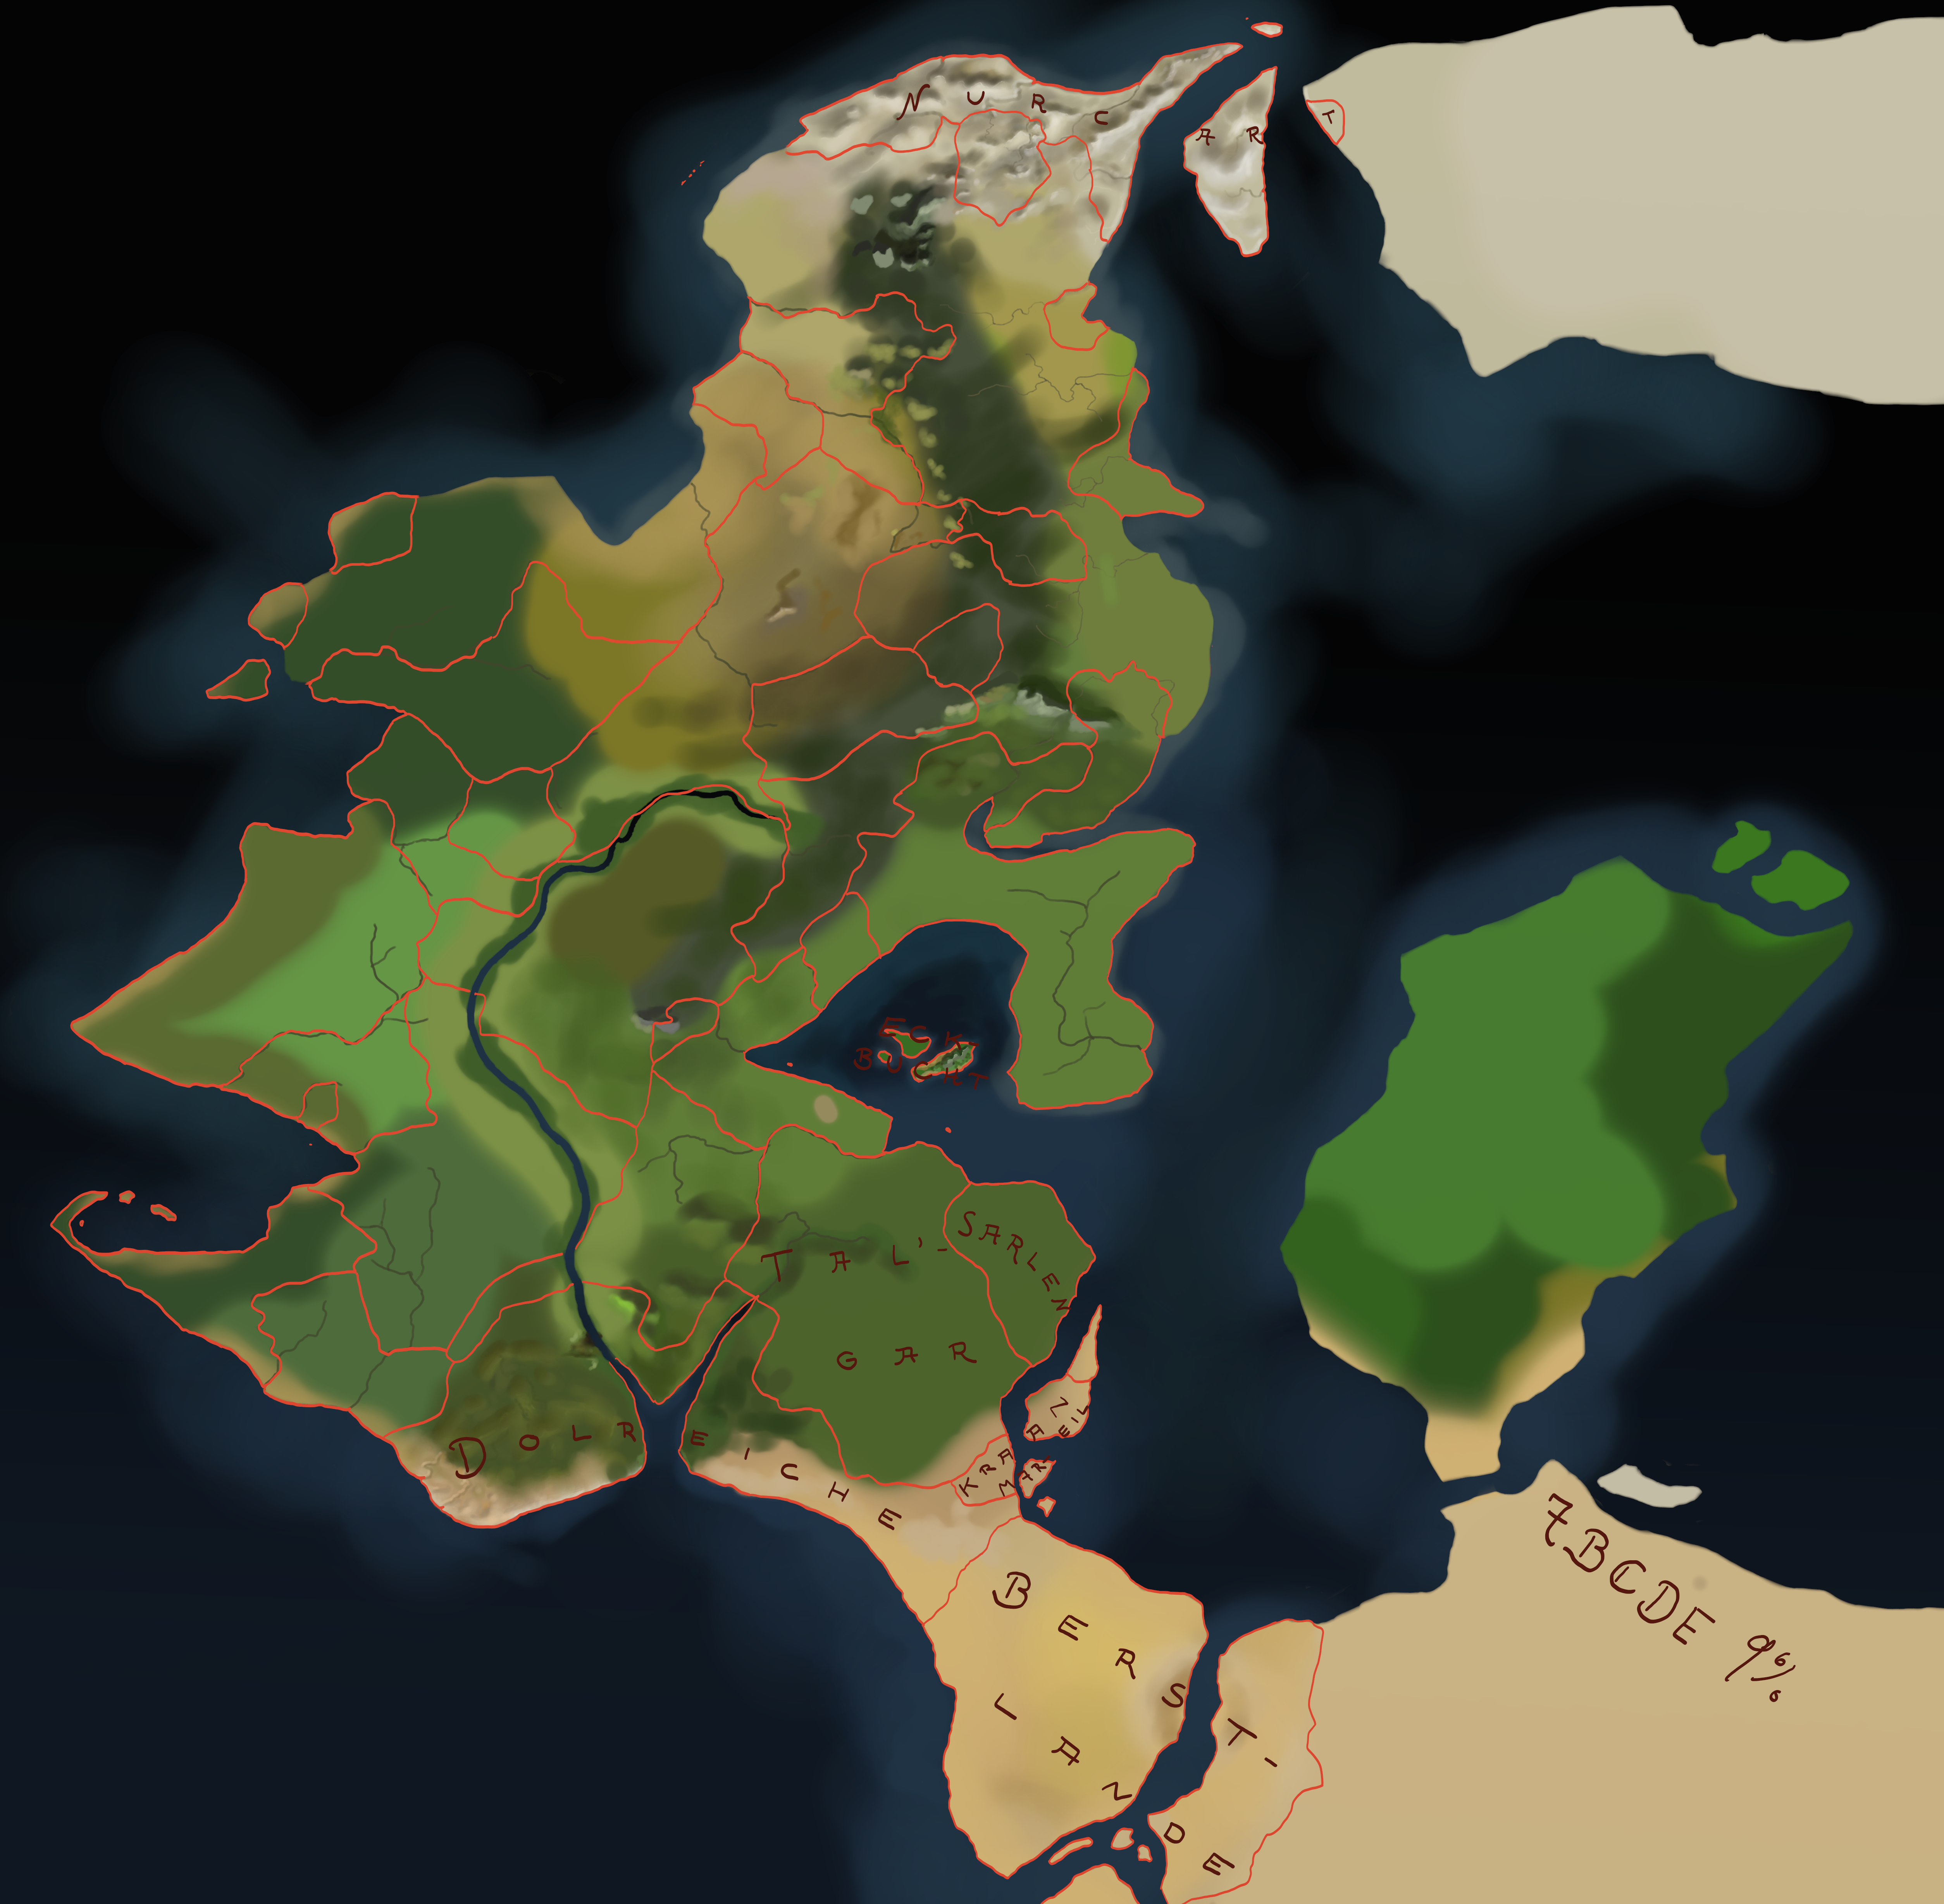
\includegraphics[width=\textwidth]{Pictures/Karte.png}
		\caption{Heimliche Lande}
        \label{fig:Heimliche_Lande}
    \end{figure*}
    
\section*{Aharsh \\ \textit{Einhorndünen}}
Eine ewige karge Ebene, bestückt mit felsigen Zähnen kalten Nächten und wenig Grün. Das rohe, riesige Gebiet im Herz der heimlichen Lande reicht von der Nahrt bis zu den Nordtiken und ist somit auch die längste \textit{regulierte} Region des Kontinents. Wobei reguliert jedoch nicht eine staatliche Verwaltung darstellt, sondern viel ehr die kulture Kategorisierung vieler hunderter Ghulstämme die über die Schluchttiefen verteilt sind, und mit eigenen Kodexen ihre Laargs (Machtgebiete) verwalten. Ohne Frage der bekannteste Stamm ist der Valc Nahk (\textit{Reiterstamm}). Das Bild der Einhörner reitenden Valc-Dorks wurde weit über die Grenzen Aharshs getragen, und sicherlich schon in vielen Malereien niedergefasst. Doch haben auch die Mrotsbauer des Ne'ekl Nahk einen präsenten Namen. Jeder zwei Mrot dieses Jahrzehnts wurde in den Händen dieser fleißigen Orks hoch oben in Ark-Arlsh entworfen, gebaut und eingeweiht. Seine es die rasanten Ratssters oder die großen Voolks, sie alle tragen die pinke Sonne der Nordtikenorks.

\section*{Amerod \\ \textit{Küste des Freiheit}}
Die Abgeschiedenen Füstentümer Amerods, schlossen sich vor 132 Jahren unter dem Banner des weißen Reißadlers zusammen. All ihr fruchtbares, verstreut besiedeltes Land unterstellten sie dem Rat der Türme in der neuen Zentralstadt Kahltenheim. Ein jedes Fürstentum erhielt proportional zu ihrer Fläche Sitze in ihm. So entsendet die Insel Chaltenhoch einen Abgesandten wärend das Fürstentum Schobersten ganze fünf Sitze inne hat. Die Abgesandten sind gewählten Repräsentanten der Menschen der Fürstentümer. Weder die Orks, Wareguards, noch die Vampire des Landes erhalten eine Möglichkeit über das Land zu entscheiden. Im Verhältniss zu den Menschen machen diese Minderheiten auch gerade mal 15\% der Bevölkerung aus. Während die Wareguards die verlassenen Höhlen des vergangenen alten Howlerimperiums im Südosten der Nation bewohnen, finden sich die Vampire im feuchteren Landesinneren, wo sie fröhlich jagen und regelmässig in Konflikte mit der menschlichen Bevölkerung geraten. Die Orks Amerods leben gemeinsam mit dem Mensch verteilt über das fruchtbaren, weite, windige Land. Die Küstenstädte Fuchtlig, Zeign und Trost sammeln die neben der Zentralstadt die meiste Bevölkerung. Ihre Häfen sind wichtige Anlegepunkte für Seefahrer und bieten den wohl besten Bierschaum des gesamten Kontinents. Von ihnen aus führt ein spärliche Netz als verschwommenden Straßen über das lose besiedelte Land. Die unregelmäßig verteilten Dörflein, sind schon von Weiten an den Drachentürmen zu erkennen. Sie verbleiben noch aus der Zeit des Feuerhimmels, als die Drachen der Aschfarbe die Neuzyklen im Süden verbracht haben und auf dem Rückweg sich mit den Winden über Amerod hinweg treiben ließen, wurde als Verteidigung gegen die regelmäßigen Dorfbrande je einer dieser Schleuder bestückten Steintürme errichtet um, wenigsten eine potentielle Gefahr darzustellen. Aus dieser Zeit stammen viele Mythen von mutigen Schützen und sterbenden Drachen.

\section*{Berstlande \\ \textit{Ewiger Stempel}}
Die kargen und vor allem heißen Berstlande markieren den südlichsten Teil der heimlichen Welt. Als einzige Region liegen diese weiten Wüsten in der “hellen Südzone”, also der Zone, die über das gesamte Jahr durchgehend im Licht Veralas liegt. Die sanften, ebenen, weiten Sandgebiete werden gespickt durch die scharfen kanten riesiger Felsbrocken, in deren mächtigen Schatten die Ruinen der alten Welt liegen. Diese Lande waren einst das Zentrum des weißen Reiches gewesen. Heute überbleiben neben verlassenen Ruinen, kleineren Kulten, der Stadt Resaîen und viele Tempel der Alten lediglich die Alten selber als Erinnerung an einen mächtige Vergangenheit.

Die in Tempel lebenden Alten, werden häufig bewacht durch Wareguards und halten sich teilweise Wiedergänger als Diener. Zudem durchstreifen Drachen die weiten Lande und vor allem die fruchtbaren Küstenbereich rund um den sauberen Schnitt auf der Suche nach Nahrung. Zu ihren Opfer zählen neben den normadisch lebenden Howlern teilweise Einhörner oder Sûrhörner (also gestachelte Minotauren). Wo der Nordwesten des Landes fast keine lebende Seele offen zeigt, ist der Südosten dank des sauberen Schnitts teilweise sogar grün. Wo der Schnitt im Süden breiter wird umläuft er die vier Inseln. Gasy, Jurr und Vian sind kleine Inseln bevölkert durch Phoenixe und Silberaffen. H’jer hingegen ist deutlich größer und felsiger. dieses heiße braun-grüne Haufen Erde wird durch die Ungeehrten bevölkert. Eine Gemeinschaft von Vampiren, Sûrhörnern und Silberaffen, mit gemischten Absichten. Mal handeln sie über Seewege mit dem Rest des Kontinents, mal stürmen sie deren Festen und plündern deren Dörfer.

Blickt man nun den sauberen Schnitt hoch nach Norden, so findet man im Osten die riesige Stadt Resaîen. Das Grabgänger- und Sûrhörnervolk wird durch ein Altenrat beherrscht und verehrt die alte Ordnung.

\section*{Dolreich \\ \textit{Drei Kronen Reich}}
Das Dolreich vereinigt die ehemaligen drei Reiche Dermisch, Ohllande und Leichsaal unter der Führung des Hauses Marl.  Im Osten erreicht das dürre Land sogar für ein kurzes Stück das L’armeer. Die primär menschliche und skrivische Bevölkerung bevölkert die Dolbucht sowohl die Nahrt als auch die Var hoch. Vereinzelt leben hier jedoch ebenso Howler, Spheroma und einige Vampire in abgelegenen Dörfern und Vereinigungen.

Das Dolreich bietet eine breite Varianz an Vegetation: Der steinige und hügelige Westen, das Pflanzen freundliche, grün-braune Zentrum und der karge, sandige Osten. Die drei ehemaligen Hauptstädte der Vorreiche bilden heute noch die Hauptknotenpunkte der Macht und des Handels:
\begin{itemize}
    \item Dermatan liegt auf der Westseite der Nahrt. Dieses Metropole ist Hauptstadt des Dolreichs, primärer Hafen des Wasserhandels und ein Kunststück der frühsiedlerischen Bauweise. Um den erhöhten und befestigten Stadtkern schlängeln sich die Spiralarme der Straßen, bestückt mit den Gebäuden der niederen Schicht. Die “Brücke” ragt vom Kern bis zur Naht und sichert somit einen direkten Zugang der hohen Herren zum Geld bringenden Wasser.
    \item Meralith ist eine wahrhaft bezaubernde Stadt. Die von starken Stadtmauern eingefasste Stadt liegt ruhig in den bebauten Hügeln des Ohllandes. Das als Bauernsiedlung gewachsene Dörfchen entwickelte sich in den dunklen Jahren zu einer Zufluchtsstelle der einfachen Bevölkerung. In den Leichenkriegen starben Großteile der Bevölkerung, so dass bis heute das schwarze Viertel verlassen im Norden der Stadt ruht.
\end{itemize}

\section*{Kraan Mareil \\ \textit{Felseninseln}}

Als die “Blutwurzeln” oder die “Höhen des kargen Tods” werden die Kraan Mareil in Sagen und Mythen umschrieben. Seit einigen tausend Jahren ist die von steinigen Höhen und trockenen Tiefen dominierte Küstenregion mit ihren Inseln Gebiet der gefürchteten Saan Mareil - den Piraten der Felsen. Von hier aus operiert die vampirische Seemacht und plant ihre nächsten Raubzüge. Die natürlichen Felsfronten bieten den leichtfüßigen Vampiren ein nahezu uneinnehmbares Territorium voller Möglichkeiten ihre perversen Folterfantasien freien Lauf zu lassen. Als Untergebene Rasse leben viele Harpyien vor allem in den Haupthäfen, um ihren übergeordneten Meistern nicht nur in Seeschlachten zur Seite zu stehen. Diese zentralen Häfen liegen sich im schwarzen Dreieck gegenüber:
\begin{itemize}
    \item Rhuus Fareii auf dem Festland ist der größte Hafen der Flotte. Die Tunnel- und Hängebrückensysteme ziehen sich tief durch das Inland und ermöglichen es so den Bewohnern schnell durch das unwegsame Gelände zu kommen.
    \item Merellee Fareii ist auf der mittleren der drei Kraan Inseln. Hier lebt vorallem der niedere Stand der Vampire in simlen Höhlen und geflochtenen Holzglocken. Die meisten Schiffe der Flotte werden in den Werten Merellee Fareiis errichtet.
    \item Saan Fareii ist der Hafen der schmutzigsten und erfolgreichesten Adeligen im Volk. Hier landen die besten Schätze und saftigsten Gefangene. Als einzigster Hafen in Kraan Mareil ist es den Harpyien hier untersagt den rauen Boden mit ihren Füßen zu beschmutzen. Verächtlich nennen sie diesen Hafen bloß “die Weiße” um die übertriebene Reinheit auszudrücken.
\end{itemize}

\section*{Sarlen \\ \textit{Schlammtäle}}

Die freien Regionen im Süden der Eckbucht werden unter dem Namen Sarlen zusammengefasst. Das schwüle, matschige Land ist unter der Kontrolle der Natur und ermöglicht es unabhängigen Sirenerotten, kleineren Minotauren Dörfern, Krograts und auch einigen Harpyien ein Leben ohne den Zwang durch Herrschaftssysteme. Jedoch bringt diese Freiheit auch Gefahren mit sich: Nicht selten kommen Jagdgruppen der Ghule hoch in den Nordosten um sich einen Rang und Namen zu verdienen. Jedoch ist auch schon das Leben ohne eine externe Gefahr hart, da ein jeder hier überleben möchte und im Zweifelsfall bereit ist über Leichen zu gehen.

\section*{Nietküste \\ \textit{Zahnrad der Zeit}}

Kaum ein Stück Land wurde so von der Flut der Skriva gezeichnet wie das windige Küstenstück zu Fuße der Schuppentiken. Gerade mal 120 Jahre nachdem die Menschen und Minotauren in den windgeschützten Neuecktälern Fuß gefasst hatten, wurden sie mit den fliehenden Skrivas in jeder Hinsicht überfordert. Egal wie gut die Ernte war, egal wie viel Land sie bieten konnten, es gab stets ein Maul zu viel und ein paar Beine zu viel. Dies war der Zeitpunkt, an dem man begann die Häuser an Felswenden in die Höhe zuziehen, das berühmt Eckbrüh an zu richten und die wiederlichen Neilfrösche auf die Speiselisten zu setzen. Selbst als die Skrivaflut abriss, und die Felder erweitert wurden, überdauerten die neu gefundenen Traditionen. Sie wurden ausgearbeitet und dank den schlauen Konzepten der Arlt-Mauer-Gemeinschaft begann der Überschwall an Fellfreunden plötzlich den Wohlstand der kleinen Nation zu beflügeln. Nicht nur sprudelten die Minearalien wie Wasser aus der Erde, sondern wurden von den Händen innovativ denkender Menschen und Skriva zu Skailen verarbeitet. Diese kunstvollen, mechanischen Konstruktionen basierten nicht auf Spiritkräften wie Mrots, sondern fanden ihren Ursprung in Mechanik und Chemischen Prozesse, was sie unabhängig von Feldverteilungen überall funktionieren ließ. Unter dem Banner des Fortschrittes und der Kooperation bildeten sich die Banken wie die \textit{Krey \& Wayne Kastbank}, Handelsgemeinschaften und die ersten Multikontinentalen Schifffahrtslinien.

\section*{Nurcart \\ \textit{Kalter Stachelpanzer}}

Nurcart ist ein kaltes erbarmungsloses Land. Es zieht sich entlang der Küste und über die schwarze Insel bis rüber über den zweiten Graben. Nurcarts Landschaft ist große Teile des Jahres mit Schnee bedeckt und stellt mit seinen schwarzen Gesteinszähnen ein kontrastreiches Bild dar. Einzelne Nadelbäume sind die kostbaren Holzquellen welche einzuteilt gewusst werden sollten.

Nurcart ist weder ein Staat noch ein Bund, sondern lediglich ein Begriff für die vielen Kreise der Cartregion. In den Kreisen leben Draekolins, Silberaffen, Minotauren, Daemonen und einige Rudel von Ghulen. Die Kreise handeln viel übers Wasser und so ist es kein Wunder, dass die größten Kreise am ersten und zweiten Graben liegen. So sind der ganz im Osten liegende K'lae Tur (Kreis der Träne), die Kreise K'lae Serk (Kreis des Eindrucks) und K'lae Kha (Kreis der Fruchtbarkeit) auf der schwarzen Insel zwar nicht auf dem Heimatkontinent, dennoch laufen zwei Drittel aller Handelsrouten des Osthandels durch die Tore dieser drei Kreise.

Jede 281ste Flut treffen sich die Kreisanführer in den 5 Region (Gaashs) um sich zu beraten. Seien es lokale Konflikte, neue Regeln, Handelspläne oder ein erneuter Marsch nach Süden um die Wildnis fern zu halten. Beim Tod eines Anführers stellt eine der 7 Gilden (Gufuars) den nächsten Anführer. Dieses Recht rotiert seit jeher durch die sieben Gufuars.

\section*{Tal’Gar \\ \textit{Invasorenreich}}

Seit Mumrak Gar 26 n.Z. als Anführer des Tal-Klans den Stahl-Klan in die Knie zwang expandierte der Klan in alle Himmelsrichtungen. Sie schlugen die Sirenen im Norden, die Minotauren an der Eckbucht, die Menschen im Westen, die Skriva im Süden und sogar die Vampire im Osten. Heute erstreckt sich das Reich der Tal’Gar zwischen dem Dolreich im Süden und der Eckbucht im Norden. Das kriegerische Ghulvolk lebt in verschiedenen Klans, welche alle dem Gar verpflichtet sind. Das heißt aber nicht, das sie wie Verbündete gemeinsam kämpfen würden. Ganz im Gegenteil. Die Rivalitäten der Ghulklans kostet jedes Jahr viele hundert Leben. Lediglich wenn der Gar die Blutfichte ergreift versammelt sich das gesammte Volk auf den Feldern des Krieges um einen neuen Schlag durchzuführen.

Zum Glück der Nachbarn ist der aktuelle Gar Kosh’ma ein recht Gold versessener Dork, welcher sich mit gewinnbringenden Verträgen zufrieden stellen lässt. Es ist jedoch nur eine Frage der Zeit, dass er seinen Platz als Gar gegen den Tod eintauschen wird - und wer der nächste Gar wird ist eine ganz andere Frage…

\section*{Valkheit \\ \textit{Herz der Ehre}}

Feuchte, begrünte Erde die unter den Fußstapfen der durch den Wald jagenden Njarkla freudig aufgeworfen wird. So wird das Land der gläubigen Orden und matschigen Straßen beschrieben. In Wahrheit ist es ehr das Land der giftigen Insekten, der großen Jagerduuns und des fröhlich Besäufnisses. Die großen Kahlteranlagen der neunzehn Orden dienen als Sammelpunkt für Handel, Schwert und Konkurenz, während in den Schatten der Schuppentiken still und heimlich das Imperium der neuen Sonne auf ersteht.
Die grüne Valkheit wird primär von den achtsamen Krograts und den machtgierigen Menschen bevölkert. Während die Schuppenechsen die feuchten Wälder sein eigen nennt, kann man den Menschen gerade im Norden des Landes antreffen. Dort stehen die großen weißen Türme Saxreiks, die Brücken Nynklas und die großen Straßen Lierens. All diese großartigen Bauwerke wurden im letzten Jahrzehnt unter dem großen Ermptus Siltran Norls erbaut, welcher nicht bloß die Infrastruktur des Nordensförderte sondern auch nach und nach einen Keil in Süden getrieben hat. Die Konflikte zwischen den innovativen Konzepten und dem gläubigen Ordenstum spannen sich längst nicht mehr nur auf Briefen und droht den mächtigen Osten der heimlichen Lande in einen Konflikt zu stürzen der sich nicht von alleine schlichten lassen wird.

\section*{Vernen \\ \textit{Das gehörnte Land}}

Kaum ein Land ist so grün, so belebt, so multikulturell der Machtspielball Vernen. Unter der Kontrolle der Nachbarnationen grünt es nun nach nach der Zeit des Westkonflikts wieder auf. Als ehemalige Ostflanke des Deutenreichs wurde es von der Herrschaft der Skrandalen befreit und ist nun Heimat für die verschiedensten Wesen. Die Ansammlungen von Skriva, Menschen, Minotauren und Wareguards die sich gemeinsam in kleinen neu geformten Zivilisationen an ein gemeinsames Feuer zwängen stehen jedoch im direkten Kontrast zu den verbrannten und niedergerissen Großstädten. Die aschebeschichteten Straßen werden noch immer von Leichensuchern begutachtet und von Bettlern überschwämmt. Sie alle haben den Preis der falschen Zeit und des falschen Ortes bezahlen müssen. Sie sehen mit wehmütigen Augen rüber in die letzte stehende Stadt: Maltena. Die junge Stadt spross einst auf der Erde der gläubigen Nunta Stämme - lose Gruppierungen von Minaotauren und Witchghulen. Als sie unter die Finger der Skrandalen fiehlen lernte sie den Bau von stabilen großen Häusern, den Umgang mit modernen Werkzeug und das bändigen der Stachelwölfe. Auch wenn heute die Stachelwölfe in den Straßen fehlen, können noch viele sehr experimentelle Mischbauten aus Stein und Holz gefunden werden, die den Beginn der Stadt markieren.
\chapter{Ausrüstung} \label{Ausrüstung}
In den Weiten der heimlichen Welt werden die Abenteuerer auf Händler, Schätze und frei vererbbaren Überbleibsel von Feinden treffen. Auch wenn man einem Wareguard keinen Rucksack anreichen wird, hat jede Kreatur zugang zu einem eigenen Inventar und der Möglichkeit Gegenstände zu transportieren. Es liegt an der Kreativität der Spieler dem Spielleiter mit nachvollziehbaren Wegen des Transport entgegenzukommen, um ihm zu erläutern wie sie ihre neuen Schätze transportieren wollen.

\section{Währungen}
In den heimlichen Landen wird ein fleißiger Sammler viele verschiedenen Währungen antreffen. Seien es die Groschen des Dolreichs, die "Knochen" der Nurcart oder die Golden der Vampire. Um Tabellenwerke zu vereinfachen nutzen wir ein Einheitswährung \textit{EW} die sich in die anderen Währungen umrechnen lässt. Sollte es die Spielergruppe stören zwischen der verschiedenen Währungen hin und her zuwechseln, kann der Spielleiter auch entscheiden ausschließlich \textit{EW} zu nutzen und so aufwendigere Listen zu umgehen. Andererseits kann es auch zu Stimmung beitragen die verschiedenen Münzen der Völker in der Hand zu haben und so Grenzübergängen eine weitere Tiefe zuzufügen.

\subsection*{Der Dolreichgroschen}
Die wichtigste Währung des Südens ist der Dolreichgroschen. Man wird ihn nicht bloß in den Dolreichen selber antreffen sondern auch in handelnden Nachbarländern antreffen. Diese sehr simple Währung besteht aus zwei Münzentypen: dem Groschen und dem Kelnen (\textit{Kleiner} im alt Delchen). Mit einem Kelnen wird man sich zwar kein Pferd kaufen können, doch falls ihr dem Jungen der euch gerade den Weg gewiesen habt ein Lächeln aufs Gesicht zaubern wollt, so wird es eine dieser zehnkanitgen Bronzemünzen tun. Ein \textbf{Kelnen} entspricht \textbf{fünf EW}. Es sind ebenfalls 20-Kelnen-Münzen im Umlauft deren feingerillter Rand das Schiff der ersten Menschen umrahmt. Da diese Münze jedoch auch für die Unterjochung der Skriva steht, wird sie nicht weiter geprägt und kann in den flaschen Situationen zu Streitigkeiten führen.
Der sehr wertvolle Groschen entspricht der monatlichen Einnahmen eines Soldaten der Reichskraft. Er erhielt bereits früh den Namen der Lohnmünze, obwohl die Soldaten ihre Bezahlung meist in Form von Kelnen bekamen. \textbf{100 Kelnen} entsprechen \textbf{einem Groschen}. Die goldene vierkantige Münze entspricht \textbf{500 EW}.

\subsection*{Die Nurcarter Knochen}
Aus dem hohen kulturellen Wert der Knochen des erlegten wild in der Historie der Nurcarter Zivilisation wird die bleiche Währung der kalten Region in Schädel, Knöchel und Zähne unterteilt.
Die dreieckigen Messingmünzen werden als \textbf{Zähne} bezeichnet und entsprechen einem Wert von \textbf{1 EW}. In der Regel kann gleichwertig auch mit echten Zähnen bezahlt werden, was die vielen zahnlosen Leichen in den alten Rauchkriegen erklärt. Ein vollen Set an Norkzähne (also \textbf{28 Stück}) wiegen \textbf{ein Knöchel} auf. \textbf{Ein Knöchel} entspricht somit \textbf{28 EW} und reicht somit für die großzahl an alltäglichen Besorgungen. Somit reicht ein Knöchel in der Regel für ein solides Abendbrot oder eine Ecke im Stall für die Nacht aus. Reiche Gäste wird man an Schädeln erkennen. \textbf{Zehn Knöchel}, \textbf{280 Zähne} oder \textbf{280 EW} entsprechen \textbf{einem} der goldenen \textbf{Schädeln}. Diese passend geformten Taler Werden gerade auf den Inseln verpöhnt und mit hochnasiger Gesellschaft assoziiert.

% - - - - - - - - - - - - - - %
% - - - - - - - - - - - - - - %

\section{Waffen} \label{waffen}
In den gefährlichen Weiten der heimlichen Landen finden sich unzählige Gründe ein Waffe zu tragen. Waffen bringen ihrem Führer erhöhte Reichweiten, einen Boni auf \textit{Schlagenaktionen} und teilweis einen weiteren Effekt ein. Sie können in verschiedene Kategorien eingeteilt werden:\\

\subsection*{Nahkampfwaffen}
Einhändige Nahkampfwaffen können eine Distanz von (Kraft/2) m weit geworfen werden und bekommen teilweise in eckigen Klammern Boni.

\subsubsection*{Hiebwaffen (1H)} \label{ar:hiebwaffe}
Unter die Kategorie der Hiebwaffen fallen die meisten einhändigen Waffen. Seien es nun Schwerter, Äxte und leichte Keulen.\\
\textbf{Kampfaktion:} \textit{Schlagen}\\
\textbf{Kosten:} 50 bis 1000 EW\\
\textbf{Bonus:} +0 bis +3, [+0 bis +1]\\
\textbf{Reichweite:} 1 m

\subsubsection*{Hieblanze (1H)} \label{ar:hieblanze}
Die 2 Meter große Axtähnliche Waffe der Nurcarter Mrots wurde von den großen Schmieden der Norks kreiert und hergestellt. Ihr Zahnradschiene ermöglicht es dem Mrot eine bewegliche Verbindung unterhalb der Hand an der Waffe zu befestigen um die Hieblanze auch einhändig verwenden zu können. An beiden Enden der Stabwaffe regt eine schmale Klinge hervor um Schwachstellen anzuvisieren und einem Gegner endgültig den Gar aus zu machen. \\
\textbf{Kampfaktion:} \textit{Schlagen}\\
\textbf{Kosten:} 3000 EW\\
\textbf{Bonus:} +4\\
\textbf{Reichweite:} 2.25 m \\
\textbf{Effekt:} Du darfst zu Beginn einer Schlagen Aktion ansagen deinen Gegner \textit{aufzuspießen}. Sowohl dein Waffenbonus, als auch all seine Rüstung- und andersartigen Verteidigungsbonis verfallen. Du erhälst in beiden Fällen den \textbf{Bonus} \textit{Element}.\\
Sollte ein Nicht Mrot diese Waffe nutzen wollen so ist sie ein Zweihänder und gibt nicht den \textit{Element}-Boni.

\subsubsection*{Pickeln (1H)}
Die Grauskriva der hohen Nav'rifberge sind bekannt für ihre brutalen Pickelkampfkünste. Die häufig in Paaren geführten Waffen sind besonders für schleichende Angriff hervoragend geeignet.\\
\textbf{Kampfaktion:} \textit{Schlagen}\\
\textbf{Kosten:} 300 bis 500 EW\\
\textbf{Bonus:} +2 bis +3\\
\textbf{Reichweite:} 0.75 m\\
\textbf{Effekt:} Schleichende Angriffe mit Picken erhalten ein zusätzlichen Bonus von +2.

\subsubsection{Sense (2H)}
Die Sense ist eines der offensichtlichsten Werkzeuge die zur Waffe umfunktioniert werden. Ihr Gefährlichkeit rührt vor allem aus der großen Fläche die sie abdecken können.\\
\textbf{Kampfaktion:} \textit{Schlagen}, \textit{\nameref{sk:niederdreschen}}\\
\textbf{Kosten:} 80 EW\\
\textbf{Bonus:} +1 \\
\textbf{Reichweite:} 1.25 m

\subsubsection*{Speere (1H oder 2H)} \label{ar:speere}
Den schlichten Speer findet man in der Hand der meisten einberufenden Soldaten. Er ist simpel, günstig und effektiv. Seine Reichweite schafft ihm zusätzlich ein Vorteil gegenüber den üblichen Hiebwaffen.\\
\textbf{Kampfaktion:} \textit{Schlagen} \\
\textbf{Kosten:} 90 EW\\
\textbf{Bonus:} +1, [+2]\\
\textbf{Reichweite:} 1.75 m\\
\textbf{Effekt:} Wird der Speer mit zwei Händen geführt so hat der Spieler Zugang zu \textit{\nameref{sk:Speerwall}}.

\begin{figure}[htbp]
		\includegraphics[width=8cm]{Pictures/Sticharm.png}
        \label{fig:Sticharm}
\end{figure}

\subsubsection*{Stichhänder (2H)} \label{ar:stichhaender}
Die wohl berühmteste Schwertart ist der Stichhänder der Nork. Diese kunstvollen grazilen Langschwerter sind als Mischung aus einem Speer und einem Schwert besonders für die Jagd auf große Kreaturen konzipiert worden.\\
\textbf{Kampfaktion:} \textit{Schlagen} \\
\textbf{Kosten:} 1500-3000 EW\\
\textbf{Bonus:} +2\\
\textbf{Reichweite:} 2 m\\
\textbf{Effekt:} Pro Größenkategorie des Gegners gibt es ein Boni/Mali von +/-2 beginnt mit +0 bei mittelgroßen Kreaturen. 

% - - - - - - - - - - - - - - %

\subsection*{Fernkampfwaffen}
Fernkampfwaffen dürfen im Nahkampf als Improvisierte Waffe benutzt werden. Sollten sie ein Bonus geben so ist dies in eckigen Klammern angegeben. Einige Waffen nutzen \textit{Munition}. Eine Spielergruppe sollte sich vor dem Spiel einigen ob z.B. Bogenschützen Listen über ihre Pfeile führen sollten oder zum Gunsten des Spielflusses dies umgangen werden soll, in dem man annimmt das der Spieler ausreichend Pfeile mit genommen hat. Munitionswaffen verschießen diese und verweilen somit in den Händen des Kämpfers. Alle anderen Fernkampfwaffen werden weggeworfen und müssen somit erst wieder eingesammelt werden.

\subsubsection*{Armbrust (2H)}
Die Armbrust wird gerne von dolreichern Soldaten und vampirischen Piraten verwendet. Ihre einfache Handhabung ermöglicht einen einfachen Umgang, mit großen Schadenspotential.\\
\textbf{Kampfaktion:} \textit{Schießen}\\
\textbf{Kosten:} 400 bis 1000 EW\\
\textbf{Bonus:} +4 bis +8, [+1]\\
\textbf{Reichweite:} 80 bis 150 m\\
\textbf{Effekt:} Munition. Die Armbrust muss nach jedem Schuss nachgeladen werden. Diese Bonusaktion kann nicht im Nahkampf ausgeführt werden.

\subsubsection*{Bogen (2H)} \label{ar:bogen}
Der Bogen ist die Waffe die am häufigsten mit dem Fernkampf verbunden wird. Je nach Ausführung und der Stärke des Schützen kann er immense Entfernungen überbrücken.\\
\textbf{Kampfaktion:} \textit{Schießen}\\
\textbf{Kosten:} 150 bis 450 EW\\
\textbf{Bonus:} +0 bis +3\\
\textbf{Reichweite:} 80 bis 110 m  PLUS (Kraft * 5) m\\
\textbf{Effekt:} Sollte mit Bögen geschlagen werden zerbrechen sie falls der Schaden mit einem Pick erfolgreich verteidigt wurde (Kein Wundenverlust).

\subsubsection*{Cnacka (1H)} \label{ar:cnacka}
\textbf{Kampfaktion:} \textit{Werfen}\\
\textbf{Kosten:} 30 EW\\
\textbf{Reichweite:} 20 m PLUS (Kraft * 5) m\\
\textbf{Effekt:} Wo auch immer der Cnacka aufschlägt wird eine Karte aufgedeckt. Bei einem Zahlenwert verlieren alle Kreaturen innerhalb von 1 m Radius dem Kartenwert entsprechend Wunden. Bei schwarzen Bildern erleiden alle Kreaturen in 1 m  Radius 10 psychische Wunden und sind \textit{\nameref{ef:geschockt}}. Das Aufdecken eines roten Bildes verteilt an alle Kreaturen in 2 m Radius das Leiden \textit{\nameref{ef:brennend}(3)}

\subsubsection*{Gebärt (2H)} \label{ar:gebärt}
Die verrückten Konstruktionen der Orks die sie Gebärte nennen, sind effektiv Scharfschützengewehre der ganz wilden Art. Sie klappern und kreischen, qualmen und verziehen sich, und doch behauptet der Ork sein Meisterwerk in Griff zu haben.\\
\textbf{Kampfaktion:} \textit{Schießen}\\
\textbf{Kosten:} 200 EW\\
\textbf{Bonus:} +(Intelligenz/5)
\textbf{Reichweite:} 60 m\\
\textbf{Effekt:} Gebärte müssen nach jedem Schuss umständlich Nachgeladen werden. Dies wird dir eine Aktion kosten.

\subsubsection*{Wurfscheiben (1H)} \label{ar:wurfscheiben}
Die scharfgeschliffenen Wurfscheiben sind sehr leichte Metallscheiben die surrend durch die Luft schießen um sich in ihre überraschten Opfer zu schneiden.\\
\textbf{Kampfaktion:} \textit{Werfen}\\
\textbf{Kosten:} 50 EW\\
\textbf{Bonus:} +2\\
\textbf{Reichweite:} Kraft + Geschicklichkeit m\\
\textbf{Effekt:} Rüstungswerte werden doppelt gegen diese Waffe angerechnet.

% - - - - - - - - - - - - - - %

\subsection*{Besondere Waffen}
Zu besonderen Waffen zählen alle möglichen Konstrukt die nicht in die oberen Kategorien fallen. Sie können mit einem in eckigen Klammern stehenden Bonus im Nahkampf verwendet werden.

\subsubsection*{Nekromantenstab} \label{ar:nekromantenstab}
Man kann kaum von den Nekromantenstäben sprechen, da sie alle einzigartig aussehen. Mal sind es mit Lungen überzogene Walrippen, mal stahlgeschmiedete Schönheiten. Doch sie alle sind zu einem Zweck in der Hand ihres Besitzers: Als Zeichen der Kontrolle über den Tod.\\
\textbf{Kampfaktion:} \textit{Spirit}-Fähigkeiten\\
\textbf{Kosten:} unbestimmbar\\
\textbf{Bonus:} +1 bis +5, [+1 bis +3]\\\\
\textbf{Effekt:} Sollten Tote oder Untote Kreaturen dem Nekromanten folgen, so tun sie dies nur sollange keine andere Person die Kontrolle über den Stab erlangt. Ansonsten folgen sie den Befehlen des neuen Meisters.

% - - - - - - - - - - - - - - %
% - - - - - - - - - - - - - - %

\section{Kleidung und Rüstung} \label{ent:kleidungundrüstung}

\begin{tcolorbox}[title= Rüstung ,colbacktitle=gray, tabulars={@{\extracolsep{\fill}\hspace{5mm}}c|c|c@{\hspace{1mm}}}, boxrule=0.5pt]
    Kettenhemd & +3 &  500 EW \\
    Schuppen Panzer & +2 & 200 EW \\
    Steppwams  & +1 & 50 EW \\
    Plattelpanzer & +4 & 1100 EW 
\end{tcolorbox}
\vspace*{0.4 cm}

\begin{tcolorbox}[title= Kleidung ,colbacktitle=gray, tabulars={@{\extracolsep{\fill}\hspace{5mm}}c|l@{\hspace{1mm}}}, boxrule=0.5pt]
    Damenstiefel & 35 EW \\
    Handschuhe & 25 EW \\
    Hemd [E] & 40 EW \\
    Lederne Hose [E] & 35 EW \\
    Mantel & 45 EW \\
    Strohhut & 20 EW \\
    Wanderstiefel [E] & 40 EW
\end{tcolorbox}
\vspace*{0.4 cm}


% - - - - - - - - - - - - - - %
% - - - - - - - - - - - - - - %

\section{Abenteuer Ausrüstung} \label{ent:abenteuerausrüstung}

\subsection*{Reiseausrüstung}

\begin{tcolorbox}[title= Reiseausrüstung,colbacktitle=gray, tabulars={@{\extracolsep{\fill}\hspace{5mm}}c|c@{\hspace{1mm}}}, boxrule=0.5pt]
    Decke & 40 EW \\
    Rucksack & 60 EW \\
    Wanderstab [+0,1 m] & 30 EW \\
    1-Mann-Zelt & 85 EW
\end{tcolorbox}
\vspace*{0.4 cm}

\subsubsection*{Feldflasche / Trinkschlauch} \label{ar:feldflaschetrinkschlauch}
Es ist essenziell am Tag genug zu trinken. \\
\textbf{Kosten:} 10 bis 60 EW, Nachfüllen:
\begin{itemize}
    \item \textbf{Wasser:} 2 EW
    \item \textbf{Bier:} 5 EW
    \item \textbf{Wein:} 10 EW
\end{itemize}
\textbf{Effekt:} Der Inhalt einer \nameref{ar:feldflaschetrinkschlauch} reicht für zwei Tage in der Wildnis. Sollte er am dritten nicht aufgefüllt oder ersetzt worden sein, so erhält die Kreatur ein Malus von -3 auf alle Eigenschaften. Dieser Effekt wiederholt sich mit jedem weiteren Tag bis eine Eigenschaft auf/unter 0 fällt und die Kreatur somit stirbt.

\subsubsection*{Landkarte}
Um sich schnell und effektiv durch unbekannte Gebiete bewegen zu können benötigt es häufig Landkarten. Je nach der Region können diese leicht zu erhalten oder in unbekannten Gefilden gar unmöglich aufzufinden sein. \\
\textbf{Kosten:} 30 bis 100 EW \\
\textbf{Effekt:} Der Besitz einer Karte sollte den Spielern einen Zugang zu den Skizze des Landes durch den Spielleiter ermöglichen. Zu dem schaffen reisende Kreaturen an einem Tag eine Distanz hin zu legen die einer Reisedauer von einer Stunde mehr entspricht.

\subsection*{Skailen}
Die Skailen sind mechanische Wunderwerke des Ostens. Sie entstanden aus den Kooperationen zwischen den talentierten Skriva und kreativen Menschen, wärend einer Zeit in der Reichtum und Luxus mehr bedeuteten als lediglich das materielle da sein, sondern auch ein Ziel und eine Perspektive dar stellten. Skailen werden in der Regel durch Federn, Schwinggewichte oder chemische Reaktionen angetrieben. Sie basieren nahezu nie auf Spiritmanifestationen und können so überall eingesetzt werden. Da es tausende von verschiedene Versionen der handgearbeiteten Stücke gibt, werden hier nur ein paar der beliebten Grundskailen auf geführt und es liegt am Erzähler sich weitere auszudenken oder diese hier zu modifizieren.

\subsubsection*{Narkta}
Narktas sind eine Form von Uhren. Im Gegen zu vielen anderen Zeitkonzepten skalieren die Zeiteinheiten der Nietküste mit der Uhrzeit. So wird die Narkta im späten Abend langsamer rotieren als im frühen Morgen. In der Regel wird der Benutzer die Uhr mit dem Sonnenaufgang neu starten müssen, da zum einen Null Uhr mit der Sonnenaufgang genormt ist und zum Anderen die antreibenden Resourcen wie eine Feder neu gespannt werden müssen. Narktas sind zwischen 200 und 700 EW wert.

% - - - - - - - - - - - - - - %

\section{Freizeit Ausrüstung}

\subsubsection*{Zirhaar}
Das Instrument der Narcarter Norks steht in einem kontroversen Widerspruch mit den Vorwürfen der Südländer das der Nork ein herzloses, barbarisches Wesen sei, das nur für den Krieg existiere. Denn auch wenn dass noch nicht einem für seine brutaleren Artgenossen stimmt, ist der Nork sehr tiefsinnig und gesellig. Wenn er zusammen mit seinen Kameraden am abendlichen Feuer sitzt und der harte Arbeit einen weiteren Tag gestrotzt hat dünstet es ihn nach einer leichten und zugleich zarten Musik. Das Zirhaar besteht aus einem sauber geschnitzen Horn von z.B. Rothörnern und Saiten von verschiedensten Tieren. Am unteren Ende des Zirhaars befindet sich eine gespannte Tierhaut, so dass der Spieler während des Zupfens mit seiner Handfläche oder dem Daumen ein ryhtmisches Schlagen erzeugen kann. \\
\textbf{Kosten:} 500 - 1500 EW

% - - - - - - - - - - - - - - %

\subsection*{Spirituele Ausrüstung}

\subsubsection*{Bund der Schritte} \label{ar:bundderschritte}
In der Zeremonie der Wegscheide wird dem Draekolin dieses Stoffbund bestückt mit Runen überreicht. Mit dem Wandel der Zeit sammelt der Draekolin Erinnerungen angesteckt an seinem Bund um sich stets seinem gelaufenen Weg bewusst zu sein um nach Hause zurückfinden zu können.
\textbf{Kosten:} 55 EW\\
\textbf{Effekt:} Wähle ein jedes Mal wenn du eine Pfadausprägung wählen darfst eine kleine Erinnerung aus deinem Umfeld, dass du ein Bund bindest. Solltest du sterben und den Bund bei dir tragen darfst du 5 der Erinnerungen Opfern um den Pfad zurück zu gehen und deine Wunden zu heilen. Dieser Effekt tritt nach ca. einer viertel Stunde ein.

\subsubsection*{Seelenfänger} \label{ar:seelenfänger}
Seelenfänger sind Ruß-Lehm-Gefäße die von herumziehenden Nekromanten verkauft und genutzt werden. Sie können die Seelen von sterbenden aufnehmen und so einem geschickten Nekromanten erlauben den Geist der Seele zu erwecken.\\
\textbf{Kosten:} 200-1000 EW\\
\textbf{Effekt:} Die erste sterbende Kreatur die diesen Behälter berührt gibt ihre Seele an den Behälter ab. Es besteht an sich keine Möglichkeit mit den gefangenen Seele zu interagieren. Mit der Zerstörung des Seelenfängers kann die Seele ihrem Gefängnis entfliehen.

% - - - - - - - - - - - - - - %
% - - - - - - - - - - - - - - %

\section{Bestandteile der Mrots} \label{ent:mrots}

\subsection*{Untersützungs-Cores} \label{core}
Um mehr Rechenleistung aus einem Mrots zu hohlen wurden Unterstützungs-Cores entwickelt. Sie bassierten auf einfachen KIs und sollen dem Mrots einfache Aufgaben abnehmen. Ein Unterstützungs-Core wäre aber niemals in der lage sich zu einem Mrots zu entwickeln.

\subsubsection*{Supcore}\label{Supcore}
Als Unterstützungscore wird der Sup core vorallem in MK-I Modellen verwendet um deren besonderes Doppelcoremodell auszunutzen.\\
\textbf{Kosten:} 2000 EW\\
\textbf{Energiebeitrag:} 8 \\
\textbf{Besonderheiten:} +1 auf alle Körperattribute

% = = = = = = = = = = = = = = = = = = = %

\subsection*{Strukturen}

\subsubsection*{MK-I Powerbox}
Die wohl am meisten vertretenste Struktur stellt die Boombox dar. Ihre besondere Doppelcoretechnologie ermöglicht es dem Mrot seinen eigenen Core auszutauschen, besonders flexibel zu sein und vorallem ganz viel Energie freizusetzen.\\
\textbf{Kosten:} 2000 EW\\
\textbf{Bewegung:} 4 \\
\textbf{Größe:} Mittel \\
\textbf{Arme:} 2 \\
\textbf{Beine:} 2 \\
\textbf{Erweiterungen:} \begin{itemize}
	    \item \textbf{Heavy:} 2
	    \item \textbf{Medium:} 2
	    \item \textbf{Light:} 1 \end{itemize}
\textbf{Besonderheiten:} Bis zu zwei Kerne.

\subsubsection*{MK-II Ranna}
Die MK-II Entwicklung hatte eine günstige vielseitig einsetzbare Maschine zu entwickeln, die leicht in großer Zahl produzierbar sein sollten.\\
\textbf{Kosten:} 1700 EW\\
\textbf{Bewegung:} 6 \\
\textbf{Größe:} Mittel \\
\textbf{Arme:} 3 \\
\textbf{Beine:} 2 \\
\textbf{Erweiterungen:} \begin{itemize}
	    \item \textbf{Medium:} 4
	    \item \textbf{Light:} 3 \end{itemize}
\textbf{Besonderheiten:} +1 auf alle Attribute.

\subsubsection*{MK-III Bietz}
Mit der Entwicklung von den Ultra-Waffen aus dem Hause Kappnert brach eine neue Ära der großen Waffen an. Um diese in die Schlacht tragen zu können wurde der MK-III entwickelt, welcher auf seinem Rücken ein super heavy Modul tragen kann.\\
\textbf{Kosten:} 3100 EW\\
\textbf{Bewegung:} 6 \\
\textbf{Größe:} Groß \\
\textbf{Arme:} 2 \\
\textbf{Beine:} 4 \\
\textbf{Erweiterungen:} \begin{itemize}
        \item \textbf{Super Heavy:} 1
	    \item \textbf{Medium:} 1
	    \item \textbf{Light:} 2 \end{itemize}
\textbf{Besonderheiten:} Das Bietz darf in seiner Bewegung schwieriges Gelände ignorieren.

\subsubsection*{MK-IV Fliesha}
Die Invasionskriege der Karlvenanlianz zwang die Orks dazu einen Weg zu finden den Kampf in die Lüfte zu tragen um ihren Gegnern ihren größten Vorteil abzunehmen. Nach einigen gescheiterten Prototypen wurde der MK-IV entwickelt. Die weiten, kantigen Flügel sind das Markenzeichen des fliegenden Konstrukts, welches aufgrund der Schwerkraft nur leichtbepackt werden kann. \\
\textbf{Kosten:} 2300 EW\\
\textbf{Bewegung:} 5 \\
\textbf{Größe:} Mittel \\
\textbf{Arme:} 2 \\
\textbf{Beine:} 3 \\
\textbf{Erweiterungen:} \begin{itemize}
	    \item \textbf{Medium:} 2
	    \item \textbf{Light:} 2 \end{itemize}
\textbf{Besonderheiten:} MK-IV Strukturen verfügen über die Fähigkeit \textit{\nameref{sk:erheben}}.


% = = = = = = = = = = = = = = = %

\subsection*{Erweiterungen: Light}

\subsubsection*{Emo-G}
Das Emo-G Modul ist eine Entwicklung des Häckler-Klans um ihre Mrots in Handelszügen mit den Dolreichern schicken zu können. Dieses kleine Kontrollmodul simuliert Gefühlsregungen und unterstützt somit soziale Interaktionen. \\
\textbf{Kosten:} 680 EW\\
\textbf{Energiebedarf:} 2 \\
\textbf{Besonderheiten:} + 2 Charisma

\subsubsection*{High-Tex-Senzor}\label{entw:high-tex}
Mit der Hilfe der Witchgoule ist es den Orks gelungen futuristische Sensor zu konstruieren, mit denen sich Ziele leichter identifizieren lassen. \\
\textbf{Kosten:} 1800 EW\\
\textbf{Energiebedarf:} 3 \\
\textbf{Besonderheiten:} + 1 Sinne und \textit{\nameref{sk:scannen}}

\subsubsection*{Infrasicht} \label{entw:infrasicht}
Das Infrasichtmodul erlaubt es seinem Träger nicht nur Photonen im menschlich sichtbaren Bereich zu Detektieren, sondern auch im Infrarotbereich. Diese ermöglicht auch in der Nacht die ein oder andere lebende Kreatur aufzuspüren.\\
\textbf{Kosten:} 1100 EW\\
\textbf{Energiebedarf:} 3 \\
\textbf{Besonderheiten:} Du kannst auch in der Dunkelheit Lebewesen aus 40 m Distanz erkennen. 

\subsubsection*{Ramhörner}\label{entw:ramhörner}
Die den Minotauren nachgeahnten Ramhörner sind stählerne Waffen die geraden beweglichen Angreifern eine zusätzlichen Vorteil in den Kampf mitbringen. \\
\textbf{Kosten:} 500 EW \\
\textbf{Energiebedarf:} 0 \\
\textbf{Besonderheiten:} In der Runde in der du eine feindliche Kreatur in einen Nahkampf bindest darfst du kostenfrei nach deiner Aktion eine Schlagenaktion ohne Waffenboni mit der obersten Deckkarte ausführen.

\subsection*{Erweiterungen: Medium}

\subsubsection*{Blizbox}
Nicht selten erwartet die mutigen Feinde der Ghule eine warm glitzende Blizbox welche sie in ihrer eigenen Rüstung grillt. \\
\textbf{Kosten:} 2000 EW\\
\textbf{Energiebedarf:} 6 \\
\textbf{Besonderheiten:} \textit{\nameref{sk:blitzentladung}} und \textit{\nameref{sk:schockladung}}

\subsubsection*{Tan-Dinx}
Wie ein Graelfar verschwimmen die riesigen Strukturen des Maschinenmonsters plötzlich mit seinem Umfeld. Man könnte schon fast erraten wem die Orks diesen Trick abgeguckt haben. \\
\textbf{Kosten:} 2750 EW\\
\textbf{Energiebedarf:} 3 \\
\textbf{Besonderheiten:} + 1 Gewandheit und \textit{\nameref{sk:tarnen}}

\subsubsection*{Truhe}
Mrots haben die Angewohnheit keine Ahnung zu haben wo sie Dinge verstauen sollen. Eine einfache eingebaute Truhe löst das Problem. \\
\textbf{Kosten:} 50 EW\\
\textbf{Besonderheiten:} Du kannst Gegenstände verstauen. Wachen wird nicht auffallen, dass dieses Versteck existiert.

\subsubsection*{Dekka-Shield}
Das Knistern eines Dekka-Shields kann so schön sein wie das Zwischern der vorbeifliegenden Vögel. Und deutlich beeindruckender. \\
\textbf{Kosten:} 2600 EW\\
\textbf{Energiebedarf:} 4 \\
\textbf{Besonderheiten:} + 2 Robustheit

\subsubsection*{V-Bow}
Die integrierte V-Bow Einheit der Killa-Serie aus 153 m.Z. wurde nach dem Fall des Grush-Klans aus den besiegten Mrots ausgebaut und unter der Führung der \textit{Krieg \& Schneider Gruppe} als Vorlage einer nun weit verbreiteten Waffe der Mrots genutzt. Dieser einfache Armbrust-ähnlicher Mechanismus, reißt die beiden Enden des Riemens auseinander und schießt so den Bolzen nach Vorne aus der Öffnung. Sobald sie sich zurück bewegen greifen die Zahnradschienen und zwingen die Bolzenhalterung zusammen mit dem Riemen zurück. Mit dem Erreichen des Haltemechanismus, drückt die Bolzenhalterung die Sicherung des nächsten Bolzen weg und er kann nachfallen. Dieser schnelle, vertrauenswürdige Mechanismus bringt den Nachteil eines geringen Schadenspotentials mit sich, ist dafür aber leicht zu handhaben. \\
\textbf{Kosten:} 1100 EW\\
\textbf{Energiebedarf:} 2 \\
\textbf{Bonus:} +1
\textbf{Reichweite:} 80 m\\
\textbf{Besonderheiten:} \textit{schießen}. Für jeden weiteren synchron schießenden V-Bow wird der Bonus verdoppelt (Es kann maximal ein Wert von +16 erreicht werden).

\subsection*{Erweiterungen: Heavy}

\subsubsection*{Greifa}
Den Entwicklern des MK-III fiel einwenig zu spät auf das ihr Mrot gar keine Arme hat. Kurzer Hand konstruierten sie daraufhin Greifa die in das Mediummodule montiert werden konnten. \\
\textbf{Kosten:} 1500 EW\\
\textbf{Energiebedarf:} 4 \\
\textbf{Besonderheiten:} + 1 Arm

\subsubsection*{Portal-Büxxe}
Auch wenn diese Energiereißertechnologie nach dem Halbzahnvorfall verboten wurden, gibt es noch immer einige dieser riskanten Teleporter auf dem Markt. \\
\textbf{Kosten:} 5000 EW\\
\textbf{Energiebedarf:} 8 \\
\textbf{Besonderheiten:} \textit{\nameref{sk:portal}}

\subsubsection*{Burna}
Schon mal gefragt wo her das Sprichwort \textit{etwas sei der Burna} kommt? Nun als die Orks erstaunt ihre Mrots fragte was dieser mächtige Flammenwand war, mit der sie eben die feinde eingeäschert hatten, antworteten die bloß: Das war der Burna! \\
\textbf{Kosten:} 2500 EW\\
\textbf{Energiebedarf:} 6 \\
\textbf{Besonderheiten:} \textit{\nameref{sk:flammeninferno}}

\subsection*{Erweiterungen: Super Heavy}

\subsubsection*{Ultra-Burna}
Nach der Einführung des Ultra-Burnas entwickelte sich eine einzigartige Grilltradition unter den nördlichen Klans unter dem Namen BBQ. \\
\textbf{Kosten:} 4100 EW\\
\textbf{Energiebedarf:} 11 \\
\textbf{Besonderheiten:} \textit{\nameref{sk:flammeninferno}} und \textit{\nameref{sk:bbq}}
\chapter{Andere Kreaturen}

\tcbset{fonttitle=\bfseries\large,fontupper=\normalsize\sffamily,colback=myred,colframe=black,colbacktitle=gray!50!white,coltitle=black, title}

Die Heimlichen Lande sind voller verschiedensten Lebensformen und Geschichten. Eine jede Spezies ist einzigartig und bringt ihre eigenen Besonderheiten mit sich.


\section*{Daera}

\begin{tcolorbox}[title= Charakteristiken,colbacktitle=mysilver, tabulars={@{\extracolsep{\fill}\hspace{1mm}}ll@{\hspace{1mm}}}, boxrule=0.5pt]
    \textbf{Gefahrenstufe:} & 2 \\
    \textbf{Erfahrungspunkte:} & 30 EP \\
    \textbf{Rasse:} & Mechanismus \\
    \textbf{Wunden:} & 26 \\
    \textbf{Blocken / Ausweichen:} & 10 / 12 \\
    \textbf{Gift / Resistenz:} & 39 / 9 \\
    \textbf{Psyche / Widerstand:} & 17 / 15 \\
    \textbf{Bewegung:} & 5 \\
    \textbf{Aktionspunkte:} & 5
\end{tcolorbox}

\begin{tcolorbox}[title= Eigenschaften, colbacktitle=mysilver, tabulars={@{\extracolsep{\fill}\hspace{1mm}}cccccc@{\hspace{1mm}}}, boxrule=0.5pt]
    \textbf{Rob} & \textbf{Gew} & \textbf{Spi} & \textbf{Ini}  & \textbf{Kra} & \textbf{Ges} \\
    10 & 12 & 11 & 10 & 11 & 17\\ \hline
    \textbf{Int} & \textbf{Cha} & \textbf{Emo} & \textbf{Krea}  & \textbf{Sin} & \textbf{Wil} \\
    11 & 17 & 7 & 14 & 4 & 15
\end{tcolorbox}

Die Daeren wurde von dem Daemon Klaerlnich und seinem ghulischen Freund Graklas erschaffen. Sie sollten zu Beginn lediglich den Lüsten der beiden genügen und sich gegenseitig in der Arena brutal auseinander nehmen. Als die Daeren jedoch effektiver wurden entschieden ihre Meister sie zu nutzen um ihre Gegner auszuschalten. Diese metallgegossenen Frauen sind sehr flink und effektiv. Seid ihrer Erschaffung 143 m.Z. stellten die beiden Erschaffer bis zu 250 Daera her. Nach ihrer Ermordung wurden ihre Metallfrauen 213 m.Z. versteigert und befinden sich heutzutage in den Händen verschiedenster mächtiger Personen.

\subsection*{Niederschlagen}
Wie eine wilde Bestie schlägt das graumetallisch glänzende Wesen an auf ihn ein zuschlagen. Immer und immer wieder. \\
\textbf{Effekt:} \textit{Passiv}. Daeras zählen mit zwei freien Händen als mit zwei Waffen ausgerüstet.

\epigraph{Sieh wie tanzen! Sieh wie sie schreien! Sie wie sie einander zerschlagen. Das ist Kunst, das ist die Zukunft mein Freund. Wir werden sie perfektionieren, zerschlagen und wieder aufbauen!}{\textit{Klaerlnich, daemonischer Psychopath}}

% _ _ _ _ _ _ _ _ _ _ _ _ _ _ _ _ %

\section*{Kriegsläufer} \label{NPC:Kriegsläufer}

\begin{tcolorbox}[title= Charakteristiken,colbacktitle=mysilver, tabulars={@{\extracolsep{\fill}\hspace{1mm}}ll@{\hspace{1mm}}}, boxrule=0.5pt]
    \textbf{Gefahrenstufe:} & 18 \\
    \textbf{Erfahrungspunkte:} & 2500 EP \\
    \textbf{Rasse:} & Mechanismus \\
    \textbf{Größe:} & gigantisch \\
    \textbf{Wunden:} & 200 \\
    \textbf{Blocken / Ausweichen:} & 19 / 5 \\
    \textbf{Gift / Resistenz:} & 41 / 19 \\
    \textbf{Psyche / Widerstand:} & 31 / 15 \\
    \textbf{Bewegung:} & 4 \\
    \textbf{Aktionspunkte:} & 5
\end{tcolorbox}

\begin{tcolorbox}[title= Eigenschaften, colbacktitle=mysilver, tabulars={@{\extracolsep{\fill}\hspace{1mm}}cccccc@{\hspace{1mm}}}, boxrule=0.5pt]
    \textbf{Rob} & \textbf{Gew} & \textbf{Spi} & \textbf{Ini}  & \textbf{Kra} & \textbf{Ges} \\
    19 & 5 & 16 & 4 & 18 & 13\\ \hline
    \textbf{Int} & \textbf{Cha} & \textbf{Emo} & \textbf{Krea}  & \textbf{Sin} & \textbf{Wil} \\
    9 & 1 & 4 & 7 & 13 & 15
\end{tcolorbox}

Der Begriff des Mrot ist zwar unglaublich dehnbar und doch hört er bei einer gewissen Größe der Konstruktion auf. Die riesigen Kriegsläufer der Nordens wurden von den Gauschtig-Orks in den Zeiten der Nordkriegen im Westen des heutigen Valreiks produziert. Ihre Herstellung wurde nach dem Friedensschluss eingestellt und nach der Einsetzung der gemischten Valarmee wurden sie als unmittelbare Gefahren des Friedens eingeschränkt. Nun findet man bloß noch vereinzelte Kriegsläufer in den Schneeebenen und in den weißen Landen. Ihre Häuser großen Körper werden von Ultracores betrieben und sind mit mächtige Belagerungswaffen ausgestattet. Auch wenn ihr Metall nach all den Jahren mit Rost befleckt wurde sind ihre mächtigen Stahlschienen noch immer ein effektiver Schutz gegen Angreifer mit natürlichen Klauen und Zähnen.

\subsection*{Schreiten}
Mit einem ununterbrochene Stapfen rückt der riesige Koloss stetig vor. Trotz des massiven Feuerns hält er seine Bewegung aufrecht und lässt sich nicht beirren. \\
\textbf{Effekt:} \textit{Passiv}. Der Kriegsläufer zählt nach seiner Bewegung als Stationär, außer ein externer Effekt behauptet etwas anderes.

\subsection*{Schwere Atelier}
\textbf{Grundwert:} 13 (Ges) + 4 (Schweres Geschütz) \\
\textbf{Reichweite:} 140 m \\
\textbf{Radius:} 2 m \\
\textbf{Effekt:} \textit{Angriff (Physisch)}. Decke eine weiter Karte auf und lege die kleinste ab. \textit{Schwere Atelier} kann nur jede zweite Runde verwendet werden.  \\

\epigraph{Ein Kreischen klang nieder von den mächtigen Bäumen die sie durch den Schneesturm sahen. Viel zu regelmäßig für einen natürlichen Ursprung. Wind sollte anders klingen. Und Bäume sollten still stehen.}{\textit{Marcberg Seissel, minotaurischer Wegführer}}

% _ _ _ _ _ _ _ _ _ _ _ _ _ _ _ _ %

\section*{Leichenfresser} \label{NPC:Leichenfresser}

\begin{tcolorbox}[title= Charakteristiken,colbacktitle=myviolet, tabulars={@{\extracolsep{\fill}\hspace{1mm}}ll@{\hspace{1mm}}}, boxrule=0.5pt]
    \textbf{Gefahrenstufe:} & 1 \\
    \textbf{Erfahrungspunkte:} & 10 EP \\
    \textbf{Rasse:} & Wiedergänger \\
    \textbf{Größe:} & mittel \\
    \textbf{Wunden:} & 25 \\
    \textbf{Blocken / Ausweichen:} & 12 / 11 \\
    \textbf{Gift / Resistenz:} & 10 / 11 \\
    \textbf{Psyche / Widerstand:} & 13 / 7 \\
    \textbf{Bewegung:} & 4 m \\
    \textbf{Aktionspunkte:} & 4
\end{tcolorbox}

\begin{tcolorbox}[title= Eigenschaften, colbacktitle=myviolet, tabulars={@{\extracolsep{\fill}\hspace{1mm}}cccccc@{\hspace{1mm}}}, boxrule=0.5pt]
    \textbf{Rob} & \textbf{Gew} & \textbf{Spi} & \textbf{Ini}  & \textbf{Kra} & \textbf{Ges} \\
    12 & 11 & 3 & 7 & 11 & 8\\ \hline
    \textbf{Int} & \textbf{Cha} & \textbf{Emo} & \textbf{Krea}  & \textbf{Sin} & \textbf{Wil} \\
    7 & 3 & 6 & 9 & 13 & 7
\end{tcolorbox}
Die Leichenfresser sind Kreaturen der Dunkelheit. Ihre blasse Haut überspannt den knochigen trägen Körper wie ein feuchtes Laken. Die missgestellten Glieder weisen noch nach Generationen von Auferstehungsiterationen die Ähnlichkeit zu ihren vorherigen Leben als Ghule im Dienste des Berstimperiums auf. Der Fluch für den so viele fehlgeleitete Kultisten des letzten Imperators ihre Seele opferten, zwingen diese arme Diener der Nation, Tag um Tag neu aufzustehen. Ihre Innereien regenerieren Nacht um Nacht im zaudern des Spiritfeldes, bis sie soweit zerfallen sind, dass selbst der Geist der Fanatiker nicht mehr erkennen kann welche Stücke zueinander gehören.\\
Diese Seelenlosen Kreaturen, kommen jede Nacht aus dem Schatten der Erde hervor um nach Leichen zum Fraß zu suchen. Denn sollten sie keine über wochen hinweg finden, würde das selbst der alte Fluch nicht in der Lage sein die materiellen Ressourcen zur Wiederherstellung zur Verfügung zu stellen. Die verzweifelten Leichenfresser gehen teilweise sogar soweit und versuchen sich daran ihr Fressen selber zu erlegen. Auch wenn dies nahezu nie Erfolg bringen wird, sehen diese Wesen keinen besseren Weg ihrem Auftrag folgen zu können. Denn wie sonst sollte das Erbe des Imperator Krailgaa erhalten bleiben?

\subsection*{Ausnehmen}
Um an physisch Ressourcen zur Regeneration zu haben benötigt der Leichenfresser Fleisch zwischen seinen Zähnen. Ob er dabei das Fleisch von Lebenden oder Toten mit seinen Reißern hervorholt spielt keine Rolle. \\
\textbf{Grundwert:} 11 (Kra) \\
\textbf{Anforderung:} Rot \\
\textbf{Reichweite:} 0.5 m \\
\textbf{Effekt:} \textit{Angriff(Physisch)}.  Heile dich um die verursachten Wunden. Dieser Angriff kann auch gegen Leichen ausgeführt werden. Hierbei würde die Anforderung \textit{Rot} gegen \textit{Stationär} getauscht werden.

\subsection*{Giftbeißer}
Die ständige Erneuerung durch den Fluch bring die Flüssigkeiten des Körpers in ganz neue Verwesungszustände. Somit wird unteranderem der Speichel zu einer sauren Mischung aus zersetzenden Substanzen, die das Verzehren von alten Fleisch vereinfachen. \\
\textbf{Effekt:} Wenn du einer Kreatur Wunden zufügst füge Ihr genauso viele Giftwunden zu.

\epigraph{Steh auf Heer des Imperiums! Richtet eure Rücken gen Himmel, und maschiert in die Zukunft! Unser Traum wärt ewig, bis die Zeit selbst vergilbt und die Erde zerbricht!}{\textit{Nic'Soul, Nekromant des letzten Imperators}}

% _ _ _ _ _ _ _ _ _ _ _ _ _ _ _ _ %

\section*{Mortak}

\begin{tcolorbox}[title= Charakteristiken,colbacktitle=mybrown, tabulars={@{\extracolsep{\fill}\hspace{1mm}}ll@{\hspace{1mm}}}, boxrule=0.5pt]
    \textbf{Gefahrenstufe:} & 5 \\
    \textbf{Erfahrungspunkte:} &  150 EP \\
    \textbf{Rasse:} & Kratzer \\
    \textbf{Größe:} & groß \\
    \textbf{Merkmale:} & \textit{\nameref{ef:schwimmer}}\\
    \textbf{Wunden:}  61 \\
    \textbf{Blocken / Ausweichen:} & 16 / 10 \\
    \textbf{Gift / Resistenz:} & 29 / 16 \\
    \textbf{Psyche / Widerstand:} & 15 / 8 \\
    \textbf{Bewegung:} & 5 \\
    \textbf{Aktionspunkte:} & 5\\
    \textbf{NK-Waffe (Klauen)}: & +2, 0.5 m
\end{tcolorbox}

\begin{tcolorbox}[title= Eigenschaften, colbacktitle=mybrown, tabulars={@{\extracolsep{\fill}\hspace{1mm}}cccccc@{\hspace{1mm}}}, boxrule=0.5pt]
    \textbf{Rob} & \textbf{Gew} & \textbf{Spi} & \textbf{Ini} & \textbf{Kra} & \textbf{Ges} \\
    16 & 10 & 3 & 6 & 18 & 7\\ \hline
    \textbf{Int} & \textbf{Cha} & \textbf{Emo} & \textbf{Krea} & \textbf{Sin} & \textbf{Wil} \\
    3 & 3 & 5 & 7 & 9 & 8
\end{tcolorbox}

In allerlei sumpfigen und feuchten Gebieten leben still und heimlich die Mortak. Die wenige Zeit die der Mortak nicht mit einem matschigen Schlaf verbringt, schleicht oder lauert er im Grünen um unvorsichtige Beute zu überraschen. Der grüne gepanzerte Rücken des Mortak eignet sich hervorragend um mit der Umgebung zu verschmelzen und selbst auf wenige Meter Abstand nicht erkannt zu werden. Sobald ihr Opfer unmittelbar vor ihnen ist überläuft der Mortak sein Opfer förmlich und reißt wenn nötig Innereien aus seinem Opfer. Sobald es tot und erlegt ist ziehen sie die Leiche zu einer abgelegenen Stelle und fressen fröhlich die Aufgeweichten Innereien. Den Restliche Körper lassen sie entweder liegen oder lassen ihn im Unterholz verschwinden.
Als sehr einsame Tiere kommt es selten dazu dass große Anzahlen an Mortaks sich in der selber Umgebung befinden. Gerade männliche Tiere fliehen tendenziell von Artgenossen, da die vergewaltigenden Weibchen ihren Geschlechtspartner umbringen um die Kinder in seinem Bauch aufwachsen und durch seine Inneren Körperteile füttern zu lassen.

%  = = = = = = = = =  %
\section*{Plünderer (Ghul)}

\begin{tcolorbox}[title= Charakteristiken, colbacktitle=myviolet, tabulars={@{\extracolsep{\fill}\hspace{1mm}}ll@{\hspace{1mm}}}, boxrule=0.5pt]
    \textbf{Gefahrenstufe:} & 1 \\
    \textbf{Erfahrungspunkte:} & 10 EP \\
    \textbf{Rasse:} & Mischling \\
    \textbf{Größe:} & mittel \\
    \textbf{Wunden:} & 40 \\
    \textbf{Schlagen ST/BW:} & 11 (+2) / 5 (+2) \\
    \textbf{Blocken / Ausweichen:} & 10 (+1) / 6 (+1)\\
    \textbf{Gift / Resistenz:} & 12 / 10 \\
    \textbf{Psyche / Widerstand:} & 11 / 6 \\
    \textbf{Bewegung:} & 5 \\
    \textbf{Aktionspunkte:} & 5 \\
    \textbf{NK-Waffe (Axt):} & +2, 1.5 m \\
    \textbf{Rüstung (Leder)}: & +1 Rüstung
\end{tcolorbox}

\begin{tcolorbox}[title= Eigenschaften, colbacktitle=myviolet, tabulars={@{\extracolsep{\fill}\hspace{1mm}}cccccc@{\hspace{1mm}}}, boxrule=0.5pt]
    \textbf{Rob} & \textbf{Gew} & \textbf{Spi} & \textbf{Ini}  & \textbf{Kra} & \textbf{Ges} \\
    10 & 6 & 6 & 8 & 11 & 5\\ \hline
    \textbf{Int} & \textbf{Cha} & \textbf{Emo} & \textbf{Krea}  & \textbf{Sin} & \textbf{Wil} \\
    4 & 6 & 7 & 10 & 6 & 6
\end{tcolorbox}

\subsection*{Schmetterschlag}
Mit einer mächtigen Bewegung nimmt der Ghul jegliche ihm zur Verfügung stehende Kraft zusammen und zwing seine rohe Waffe nieder gen Boden. Einem Regen aus Stahl, Blut und Stückchen zerschellt sie an dem triefende Aufprall am Gegner. \\
\textbf{Grundwert:} Kraft \\
\textbf{Anforderungen:} $\Kreuz{}$ \\
\textbf{Reichweite:} 0.5 m \\
\textbf{Effekt:}  Verbrauche einen weiteren Aktionspunkt. \textit{Angriff (Physisch)}. Ignoriere die Rüstungs/Schild Bonis der Kreatur. Falls eine Waffe für diese Aktion verwendet wird Zerbricht diese (nur Nahkampfwaffen können genutzt werden) falls die oberste Karte ein Kreuz ist richtet dabei Wunden in Höhe des Bonuses an.

\subsection*{Wutanfall}
Emotionen spielen eine zentralle Rolle im Leben der Ghule. Sie lieben das Gefühl von Dominanz, sie hassen die Hilflosigkeit und sie können echt wütend werden. Eine solch wütende Kreatur in den Feindreihen zu sehen, bringt einen schnell dazu seine Pläne um zu ändern. \\
\textbf{Grundwert:} Emotionen \\
\textbf{Anforderungen:} $\Herz{}$ 16+ \\
\textbf{Effekt:} \textit{Angriff (Psyche)}: Falls die Kreatur diese Aktionsrunde noch nicht dran war, kannst du dich entscheiden keinen Schaden zu machen, dafür muss die Kreatur in seiner nächsten Aktionsphase eine Vorausplannen Aktion durchführen. 
% _ _ _ _ _ _ _ _ _ _ _ _ _ _ _ _ %

%  = = = = = = = = =  %
\section*{Plünderer (Mensch)}

\begin{tcolorbox}[title= Charakteristiken, colbacktitle=myskin, tabulars={@{\extracolsep{\fill}\hspace{1mm}}ll@{\hspace{1mm}}}, boxrule=0.5pt]
    \textbf{Gefahrenstufe:} & 1 \\
    \textbf{Erfahrungspunkte:} & 10 EP \\
    \textbf{Rasse:} & Mischling \\
    \textbf{Größe:} & mittel \\
    \textbf{Wunden:} & 37 \\
    \textbf{Schlagen ST/BW:} & 8 (+1) / 8 (+1) \\
    \textbf{Blocken / Ausweichen:} & 8 (+1) / 8 (+1) \\
    \textbf{Gift / Resistenz:} & 10 / 8 \\
    \textbf{Psyche / Widerstand:} & 10 / 8 \\
    \textbf{Bewegung:} & 5 \\
    \textbf{Aktionspunkte:} & 5 \\
    \textbf{NK-Waffe (Schwert):} & +1, 1 m \\
    \textbf{NK-Fernkampf (Kurzbogen)}: & +1, 20 m \\
    \textbf{Rüstung (Leder)}: & +1 Rüstung
\end{tcolorbox}

\begin{tcolorbox}[title= Eigenschaften, colbacktitle=myskin, tabulars={@{\extracolsep{\fill}\hspace{1mm}}cccccc@{\hspace{1mm}}}, boxrule=0.5pt]
    \textbf{Rob} & \textbf{Gew} & \textbf{Spi} & \textbf{Ini}  & \textbf{Kra} & \textbf{Ges} \\
    8 & 8 & 5 & 10 & 8 & 8\\ \hline
    \textbf{Int} & \textbf{Cha} & \textbf{Emo} & \textbf{Krea}  & \textbf{Sin} & \textbf{Wil} \\
    5 & 8 & 6 & 9 & 4 & 8
\end{tcolorbox}

\subsection*{Koordinierter Angriff}
Mit schnellen, präzisen Angriffen kann selbst ein übermächtiger Feind in die Knie gezwungen werden.\\
\textbf{Grundwert:} Intelligenz \\
\textbf{Anforderung:} $\Karo{}$ 15+\\
\textbf{Reichweite:} 10 m \\
\textbf{Effekt:} Braucht an stelle von 1em 3 Aktionspunkte. Bestimme ein Ziel jede befreundete Kreatur in Reichweite zur gewählten Kreatur (du auch) darf eine Schlagen (Werfen oder Schießen) Probe durchführen.

\subsection*{Taktieren}
Mit seinen vorsichtigen Vorgehensweisen ist der Mensch häufig zurückhaltend und schätzt sein Leben über dem Tod seines Feindes.\\
\textbf{Grundwert:} Intelligenz \\
\textbf{Anforderung:} Stationär $\Kreuz{}$ 15+ \\
\textbf{Effekt:} Befreundete Kreaturen im 10 m Radius haben die nächste Aktionsphase kostenlos Verketten bei ihren Aktionen.
% _ _ _ _ _ _ _ _ _ _ _ _ _ _ _ _ %

\section*{Rothorn}

\begin{tcolorbox}[title= Charakteristiken,colbacktitle=mybrown, tabulars={@{\extracolsep{\fill}\hspace{1mm}}ll@{\hspace{1mm}}}, boxrule=0.5pt]
    \textbf{Gefahrenstufe:} & 3 \\
    \textbf{Erfahrungspunkte:} & 55 EP \\
    \textbf{Rasse:} & Kratzer \\
    \textbf{Größe:} & groß \\
    \textbf{Wunden:} & 43 \\
    \textbf{Blocken / Ausweichen:} & 9 / 14 \\
    \textbf{Gift / Resistenz:} & 10 / 9 \\
    \textbf{Psyche / Widerstand:} & 5 / 7 \\
    \textbf{Bewegung:} & 6 \\
    \textbf{Aktionspunkte:} & 4\\
    \textbf{NK-Waffe (Hörner)}: & +1, 1 m
\end{tcolorbox}

\begin{tcolorbox}[title= Eigenschaften, colbacktitle=mybrown, tabulars={@{\extracolsep{\fill}\hspace{1mm}}cccccc@{\hspace{1mm}}}, boxrule=0.5pt]
    \textbf{Rob} & \textbf{Gew} & \textbf{Spi} & \textbf{Ini}  & \textbf{Kra} & \textbf{Ges} \\
    9 & 14 & 7 & 9 & 10 & 12\\ \hline
    \textbf{Int} & \textbf{Cha} & \textbf{Emo} & \textbf{Krea}  & \textbf{Sin} & \textbf{Wil} \\
    8 & 7 & 8 & 4 & 12 & 7
    
\end{tcolorbox}
Wie fleischgewordene Albträume werden die zwei Meter große Hirschwesen beschrieben. Diese scheuen Einzelgänger versuchen Kontakt zu anderen Rassen so gering wie möglich  zu halten. Untereinander sind Rothörner zutrauig und teilen offen Nahrungsquellen, Informationen und vor allem Sagen. Wie faszinierte Kinder lieben die Rothörner Geschichten von mächtigen Horngenossen. In der Regel wird dem Gastgebenden Rothorn die Ehre teil Geschichten zu erzählen. Dafür wird ihm gedankt und ihm wird die Ehre der Wahl des Geschlechtsverkehrspatners für die Nacht offengelegt.
Das Rothorn ernährt sich rein vegetarisch und nutzt seine Krallenfinger um ihre Nahrung aus Vertiefungen zu kratzen.

\subsection*{Fluchtverhalten}
Rothörner kämpfen nie wenn sie keine Chance auf Erfolg sehen. Lieber würden sie sich gefangen nehmen lassen oder, was ihnen am liebsten ist, fliehen. \\
\textbf{Effekt:} \textit{Passiv}. Jedes Mal wenn eine befreundetes Rothorn stirbt macht das Rang höchste Rothorn eine Willenskraftprobe(9+) mit einem Mali von -3 pro gefallenes Rothorn. Sollte sie missglücken fliehen die Rothörner. Wenn das nicht möglich ist versuchen sie sich zu unterwerfen.

\subsection*{Gut vernetzt}
Ein Rothorn läuft selten alleine durch die Wälder. Wenn sie in Panik verfallen rufen sie ihre Artgenossen um eine Chance zu erhalten mit dem Leben davonzu kommen.\\
\textbf{Grundwert:} 7 (Cha)\\
\textbf{Anforderung:} 18 +\\
\textbf{Effekt:} Ein weiteres Rothorn tritt nächste Kampfrunde dem Kampf bei. Kann nur einmal jede Kampfrunde von einem beliebigen Rothorn verwendet werden. Es treten außerhalb ihrer Heimat maximal 3 weitere Rothörner der Kampf bei.

\epigraph{Die Hörner vom Rothorn kann man sich toll an die Wand hämmr'n. Wenn du welche findest natürlich! \textit{Gelächter} Die Drecksdinge sind schnell. Echt schnell. Die sinn sogar dem Mark'i wech gelaufen.}{\textit{Murkat der Steinschmeisser, dorkischer Krieger}}

% _ _ _ _ _ _ _ _ _ _ _ _ _ _ _ _ %

\section*{Schattenvard}

\begin{tcolorbox}[title= Charakteristiken, colbacktitle=mydarkblue, tabulars={@{\extracolsep{\fill}\hspace{1mm}}ll@{\hspace{1mm}}}, boxrule=0.5pt]
    \textbf{Gefahrenstufe:} & 2 \\
    \textbf{Erfahrungspunkte:} & 25 EP \\
    \textbf{Rasse:} & Spirit \\
    \textbf{Größe:} & mittel \\
    \textbf{Wunden:} & 28 \\
    \textbf{Blocken / Ausweichen:} & 6 / 13 \\
    \textbf{Gift / Resistenz:} & 11 / 6 \\
    \textbf{Psyche / Widerstand:} & 12 / 7 \\
    \textbf{Bewegung:} & 6 \\
    \textbf{Aktionspunkte:} & 5 \\
    \textbf{NK-Waffe (Rückengarne):} & +1, 4 m \\
    \textbf{NK-Waffe (Krallen)}: & +2, 0.5 m
\end{tcolorbox}

\begin{tcolorbox}[title= Eigenschaften, colbacktitle=mydarkblue, tabulars={@{\extracolsep{\fill}\hspace{1mm}}cccccc@{\hspace{1mm}}}, boxrule=0.5pt]
    \textbf{Rob} & \textbf{Gew} & \textbf{Spi} & \textbf{Ini}  & \textbf{Kra} & \textbf{Ges} \\
    6 & 13 & 11 & 9 & 5 & 15\\ \hline
    \textbf{Int} & \textbf{Cha} & \textbf{Emo} & \textbf{Krea}  & \textbf{Sin} & \textbf{Wil} \\
    8 & 7 & 8 & 4 & 9 & 7
\end{tcolorbox}

Die schlanke, humanoide Gestalt der Schattenvard ist verbunden mit Krallenfüßen, einem vogelähnlichen Kopf und zwei flache Rückengarnen. Mit schnellen athletischen Manövern ist die Schattenvard in der Lage Gegner in den Rücken zu fallen und sie ausfindig zu machen. Als Vard ist die Schattenvard in der Lage Spirit zu manifestieren und die Beweggründe ihrer Feinde zu erkennen. Mit ihren bis zu zwei Meter langen Rückengarnen kann sie gemeine Schläge ausführen oder ihre Gegner festsetzen. Die Schattenvarde leben häufig als Begleiter von Kultisten der Gri oder im Dienste von gläubigen Dienstherren.

\subsection*{Auslesen}
Als wüsste der Schattenvard exakt was sie tun würde konterte sie die Schläge, wich dem Tritt aus und Schlug überlegen zurück.\\
\textbf{Grundwert:} 11 (Spi) - 4\\
\textbf{Anforderung:} Int[Ziel]+\\
\textbf{Reichweite:} 10 m \\
\textbf{Effekt:} Die Zielkreatur legt seine beste Handkarte ab und zieht eine neue Karte. Falls es keine Spielerkreatur ist, erleidet die Kreatur 5 Psychischen Schaden.

\subsection*{Federnde Sprünge}
Als gäbe es keine Schwerkraft schleudern sich die Schattenvarde von Türmen und Klippen, über Gemäuer und Feinde hinein in das Getümmel.\\
\textbf{Effekt:} \textit{Passiv}. Ignoriere Gelände und Feinde während deiner Bewegung, vorausgesetzt deine Endposition ist frei. Du zählst, solang keine Effekte etwas anderes verlangen, immer als in Bewegung.

\subsection*{Schattenbolzen}
Das Dartförmige Geschoss zieht flatternd einen schwarzen Schweif hinter sich her. Der schwere Aufschlag passt weniger zum grazilen Schuss und errinnert viel ehr an einen nieder schmetternden Hammer. \\
\textbf{Grundwert:} 11 (Spi) + 3\\
\textbf{Anforderung:} 16+\\
\textbf{Reichweite:} 45 m \\
\textbf{Effekt:} \textit{Angriff(Physisch)}. Erleidet ein Bewegtes Ziel Wundenverluste durch Schattenbolzen, so verliert diese Kreatur eine Handkarte/einen Aktionspunkt.

\epigraph{Ich weiß es nicht, meine Herrin. Sie war sehr schnell und sprangen mit Leichtigkeit von Turm zu Turm. Sie liefen die im Schatten der Nacht und ich hatten keine Möglichkeit sie genauer zu betrachten. Als sie bei ihrem Gatten ins Zimmer sprang hörte ich nur noch seine überraschte Stimme. Wie sie abbrach...}{\textit{Larissa Meinla, menschliche Rattenfängerin}}

\subsection*{}

% _ _ _ _ _ _ _ _ _ _ _ _ _ _ _ _ %

\section*{Skriva}

\begin{tcolorbox}[title= Charakteristiken, colbacktitle=mygreen, tabulars={@{\extracolsep{\fill}\hspace{1mm}}ll@{\hspace{1mm}}}, boxrule=0.5pt]
    \textbf{Gefahrenstufe:} & 2 \\
    \textbf{Erfahrungspunkte:} & 5 EP \\
    \textbf{Rasse:} & Kratzer \\
    \textbf{Größe:} & mittel \\
    \textbf{Wunden:} & 32 \\
    \textbf{Schlagen ST/BW:} & 6 (+1) / 12 (+1) \\
    \textbf{Blocken / Ausweichen:} & 6 (+1) / 10 (+1) \\
    \textbf{Gift / Resistenz:} & 14 / 6 \\
    \textbf{Psyche / Widerstand:} & 9 / 5 \\
    \textbf{Bewegung:} & 5 \\
    \textbf{Aktionspunkte:} & 5 \\
    \textbf{NK-Waffe (Krallen)}: & +1, 0.5 m \\
    \textbf{Rüstung (Chitin)}: & +1
\end{tcolorbox}

\begin{tcolorbox}[title= Eigenschaften, colbacktitle=mygreen, tabulars={@{\extracolsep{\fill}\hspace{1mm}}cccccc@{\hspace{1mm}}}, boxrule=0.5pt]
    \textbf{Rob} & \textbf{Gew} & \textbf{Spi} & \textbf{Ini}  & \textbf{Kra} & \textbf{Ges} \\
    6 & 10 & 9 & 11 & 6 & 12 \\ \hline
    \textbf{Int} & \textbf{Cha} & \textbf{Emo} & \textbf{Krea}  & \textbf{Sin} & \textbf{Wil} \\
    6 & 3 & 5 & 3 & 9 & 5
\end{tcolorbox}

\subsection*{Säurespeien}
Als wahrer Allesfresser benötigen die Skriva besondere Säuren um mit den Fremdkörpern klar zu kommen. Wenn diese Säuren jedoch ausgespuckt werden sind sie umso schrecklicher.\\
\textbf{Grundwert:} 12 (Gesch) \\
\textbf{Anforderung:} 18+ \\
\textbf{Effekt:} \textit{Angriff (Gift)}. Reduziere die Rüstung des Ziels um \textbf{FK}. \textbf{Bonus:} Toxin.

\subsection*{Toxinstich}
Mit einer flinken Bewegung sticht der wendige Skriva seinen Klauenbesetzen Schwanz in die Organe seines Gegners. Das übertragende Gift kann nun frei im langsam zerfallenden Körper propagieren.\\
\textbf{Grundwert:} 12 (Gesch) \\
\textbf{Anforderung:} Bewegt \\
\textbf{Reichweite:} 0.75 m \\
\textbf{Effekt:} \textit{Angriff (Gift)}. Sollte eine Kreatur Giftwunden erleiden, so erleidet sie den Effekt deines Giftes. \textbf{Bonus:} Toxin.

\subsection*{Volk der Unterwelt}
Durch ihr Leben in der dunklen Unterwelt haben die Skriva ihren Sehsinn optimiert.\\
\textbf{Effekt:} \textit{Passive.} Du kannst in Dämmerung auf 50 m noch normal sehen und in Dunkelheit 30 m. Allerdings bist du leicht zu blenden.

% _ _ _ _ _ _ _ _ _ _ _ _ _ _ _ _ %

\section*{Skriva (Schwarmführer)}

\begin{tcolorbox}[title= Charakteristiken, colbacktitle=mygreen, tabulars={@{\extracolsep{\fill}\hspace{1mm}}ll@{\hspace{1mm}}}, boxrule=0.5pt]
    \textbf{Gefahrenstufe:} & 3 \\
    \textbf{Erfahrungspunkte:} & 30 EP \\
    \textbf{Rasse:} & Kratzer \\
    \textbf{Größe:} & mittel \\
    \textbf{Wunden:} & 42 \\
    \textbf{Schlagen ST/BW:} & 9 (+2) / 15 (+2) \\
    \textbf{Blocken / Ausweichen:} & 9 (+3) / 13 (+3) \\
    \textbf{Gift / Resistenz:} & 19 / 9 \\
    \textbf{Psyche / Widerstand:} & 14 / 9 \\
    \textbf{Bewegung:} & 5 \\
    \textbf{Aktionspunkte:} & 5 \\
    \textbf{NK-Waffe (Krallen)}: & +2, 0.5 m \\
    \textbf{Rüstung (Chitin)}: & +3
\end{tcolorbox}

\begin{tcolorbox}[title= Eigenschaften, colbacktitle=mygreen, tabulars={@{\extracolsep{\fill}\hspace{1mm}}cccccc@{\hspace{1mm}}}, boxrule=0.5pt]
    \textbf{Rob} & \textbf{Gew} & \textbf{Spi} & \textbf{Ini}  & \textbf{Kra} & \textbf{Ges} \\
    9 & 13 & 12 & 14 & 9 & 15 \\ \hline
    \textbf{Int} & \textbf{Cha} & \textbf{Emo} & \textbf{Krea}  & \textbf{Sin} & \textbf{Wil} \\
    10 & 5 & 8 & 5 & 12 & 9
\end{tcolorbox}

\subsection*{Säurespeien}
Als wahrer Allesfresser benötigen die Skriva besondere Säuren um mit den Fremdkörpern klar zu kommen. Wenn diese Säuren jedoch ausgespuckt werden sind sie umso schrecklicher.\\
\textbf{Grundwert:} 15 (Gesch) \\
\textbf{Anforderung:} 18+ \\
\textbf{Effekt:} \textit{Angriff (Gift)}. Reduziere die Rüstung des Ziels um \textbf{FK}. \textbf{Bonus:} Toxin.

\subsection*{Schattenläufer}
Die Skriva sind seid Generationen schon Kreaturen der Schatten. Auch wenn sie nicht unter offenen Bereichen leiden fühlen sie sich schnell ungedeckt und unwohl. Im Gegenzug sind sie jedoch hervoragende Jäger in den Schatten und unglaublich schwer auszumachen, wenn sie nicht gesehen werden wollen.
\textbf{Grundwert:} 13 (Gew) \\
\textbf{Anforderung:} 18 +\\
\textbf{Effekt:} Du musst dich innerhalb von einem Meter Entfernung von einem Objekt befinden das min. eine Größenortnung größer als du ist. Du tarnst dich und erhälst somit einen Bonus von 8 auf deine Verteidigung. Sobald du Wunden erleidest, eine Aktion außerhalb eines Schatten bzw. im Nahkampf mit einer Kreatur beendest oder selber angreifst, verblasst die Tarnung. Erhalte ein Vorteil.

\subsection*{Toxinwolke}
Das närrische Funkeln der Vorfreude in den Augen eines Skrivas bedeutet seltens etwas gutes. Hört man Sekunden später ein sanftes Zischens, richt schwefelartige Gerüche und sieht ein ungleichmäßig verteiltes Grün aufsteigen, so weiß man dass man definitiv nicht atmen sollte! \\
\textbf{Grundwert:} 12 (Spi) \\
\textbf{Anforderung:} Stationär \& $\Karo{}$ 18 +\\
\textbf{Radius:} 1 m \\
\textbf{Effekt:} Alle Kreaturen innerhalb des Wirkungsradius müssen eine Robustheitsprobe (17+) bestehen oder werden Opfer deines aktiven Gifts.
\textbf{Bonus:} Toxin.

\subsection*{Toxinstich}
Mit einer flinken Bewegung sticht der wendige Skriva seinen Klauenbesetzen Schwanz in die Organe seines Gegners. Das übertragende Gift kann nun frei im langsam zerfallenden Körper propagieren.\\
\textbf{Grundwert:} 15 (Gesch) \\
\textbf{Anforderung:} Bewegt \\
\textbf{Reichweite:} 0.75 m \\
\textbf{Effekt:} \textit{Angriff (Gift)}. Sollte eine Kreatur Giftwunden erleiden, so erleidet sie den Effekt deines Giftes. \textbf{Bonus:} Toxin.

\subsection*{Volk der Unterwelt}
Durch ihr Leben in der dunklen Unterwelt haben die Skriva ihren Sehsinn optimiert.\\
\textbf{Effekt:} \textit{Passive.} Du kannst in Dämmerung auf 50 m noch normal sehen und in Dunkelheit 30 m. Allerdings bist du leicht zu blenden.

% _ _ _ _ _ _ _ _ _ _ _ _ _ _ _ _ %

\section*{Takdisha Kompan} \label{npc:takdisha Kompan}

\begin{tcolorbox}[title= Charakteristiken, colbacktitle=mysilver, tabulars={@{\extracolsep{\fill}\hspace{1mm}}ll@{\hspace{1mm}}}, boxrule=0.5pt]
    \textbf{Gefahrenstufe:} & 1 \\
    \textbf{Erfahrungspunkte:} & 25 EP \\
    \textbf{Rasse:} & Mechanismus \\
    \textbf{Größe:} & klein \\
    \textbf{Wunden:} & 19 \\
    \textbf{Blocken / Ausweichen:} & 10 / 9 \\
    \textbf{Gift / Resistenz:} & 11 / 10 \\
    \textbf{Psyche / Widerstand:} & 9 / 10 \\
    \textbf{Bewegung:} & 4 \\
    \textbf{Aktionspunkte:} & 5 \\
    \textbf{NK-Waffe (Gefährliche Kanten):} & -1, 0.25 m \\
\end{tcolorbox}

\begin{tcolorbox}[title= Eigenschaften, colbacktitle=mydarkblue, tabulars={@{\extracolsep{\fill}\hspace{1mm}}cccccc@{\hspace{1mm}}}, boxrule=0.5pt]
    \textbf{Rob} & \textbf{Gew} & \textbf{Spi} & \textbf{Ini}  & \textbf{Kra} & \textbf{Ges} \\
    10 & 9 & 5 & 7 & 6 & 11\\ \hline
    \textbf{Int} & \textbf{Cha} & \textbf{Emo} & \textbf{Krea}  & \textbf{Sin} & \textbf{Wil} \\
    9 & 12 & 16 & 6 & 10 & 8
\end{tcolorbox}

Freche Münder würden sie als kleine, planlose Maschinen bezeichnen, aber sie sind \textit{mehr}! Diese kleine Konstruktionen von angehende Witchghulen sind Wunderwerker fantastischer Fantasie. Ihre Funkelcores sind aggressiv zusammengepresste Schwarzkerne deren pure Überkonzentration an Spiritszündungen den Minimrot mit Energie überströmen. Der \textit{Takdisha Kompan} erhält eine mittlere Erweiterung oder zwei leichte Erweiterungen.

% _ _ _ _ _ _ _ _ _ _ _ _ _ _ _ _ %

\section*{Terror Hund}

\begin{tcolorbox}[title= Charakteristiken, colbacktitle=myviolet, tabulars={@{\extracolsep{\fill}\hspace{1mm}}ll@{\hspace{1mm}}}, boxrule=0.5pt]
    \textbf{Gefahrenstufe:} & 1 \\
    \textbf{Erfahrungspunkte:} & 5 EP \\
    \textbf{Rasse:} & Wiedergänger \\
    \textbf{Größe:} & klein \\
    \textbf{Wunden:} & 21 \\
    \textbf{Blocken / Ausweichen:} & 5 / 9 \\
    \textbf{Gift / Resistenz:} & 6 / 5 \\
    \textbf{Psyche / Widerstand:} & 6 / 6 \\
    \textbf{Bewegung:} & 6 \\
    \textbf{Aktionspunkte:} & 4 \\
\end{tcolorbox}

\begin{tcolorbox}[title= Eigenschaften, colbacktitle=myviolet, tabulars={@{\extracolsep{\fill}\hspace{1mm}}cccccc@{\hspace{1mm}}}, boxrule=0.5pt]
    \textbf{Rob} & \textbf{Gew} & \textbf{Spi} & \textbf{Ini}  & \textbf{Kra} & \textbf{Ges} \\
    5 & 9 & 3 & 11 & 5 & 8\\ \hline
    \textbf{Int} & \textbf{Cha} & \textbf{Emo} & \textbf{Krea}  & \textbf{Sin} & \textbf{Wil} \\
    7 & 6 & 8 & 5 & 11 & 6
\end{tcolorbox}
Dies sind keine normalen Untoten Hunde, es sind solche die durch spezielle Riten zu Tötungmaschienen gemacht wurden. Sie jagen alles was sich bewegt.\\

\subsection*{Flink}
Die geringe Größe kombiniert mit den schnellen Pfoten ermöglichen dem hungrigen Terrorwolf schnelle Manöver und unvorhergesehene Haken.\\
\textbf{Effekt:} \textit{Passiv}. Kann sich ohne Gegenschläge aus dem Nahkampf entfernen.

\subsection*{Rudelkämpfer}
........\\
\textbf{Effekt:} \textit{Passiv}. Für jeden Verbündeten der sich im Nahkampfreichweite deines Ziels befindet erhalte einen Bonus von +3 auf Angriffe.

% _ _ _ _ _ _ _ _ _ _ _ _ _ _ _ _ %

\section*{Treant}

\begin{tcolorbox}[title= Charakteristiken, colbacktitle=mydarkblue, tabulars={@{\extracolsep{\fill}\hspace{1mm}}ll@{\hspace{1mm}}}, boxrule=0.5pt]
    \textbf{Gefahrenstufe:} & 2 \\
    \textbf{Erfahrungspunkte:} & 20 EP \\
    \textbf{Rasse:} & Spirit \\
    \textbf{Größe:} & groß \\
    \textbf{Wunden:} & 41 \\
    \textbf{Schlagen ST/BW:} & 13 / 7 \\
    \textbf{Blocken / Ausweichen:} & 14 / 7 \\
    \textbf{Gift / Resistenz:} & 15 / 14 \\
    \textbf{Psyche / Widerstand:} & 12 / 5 \\
    \textbf{Bewegung:} & 4 \\
    \textbf{Aktionspunkte:} & 5 \\
\end{tcolorbox}

\begin{tcolorbox}[title= Eigenschaften, colbacktitle=mydarkblue, tabulars={@{\extracolsep{\fill}\hspace{1mm}}cccccc@{\hspace{1mm}}}, boxrule=0.5pt]
    \textbf{Rob} & \textbf{Gew} & \textbf{Spi} & \textbf{Ini}  & \textbf{Kra} & \textbf{Ges} \\
    14 & 7 & 12 & 5 & 13 & 7\\ \hline
    \textbf{Int} & \textbf{Cha} & \textbf{Emo} & \textbf{Krea}  & \textbf{Sin} & \textbf{Wil} \\
    7 & 3 & 6 & 9 & 13 & 5
\end{tcolorbox}
Treants sind Bäume die eine tiefe Verbindung mit dem Spiritfeld haben und zum Leben erwacht sind. 
Da sie ein Band nicht nur unter sich sondern mit allen Bäumen haben merken sie sofort wenn im Wald etwas vor sich geht.\\

\subsection*{Verwurzelt}
........\\
\textbf{Effekt:} \textit{Passiv}. Wenn du stehst bist du verwurzelt und kannst nicht bewegt werden.

\subsection*{Waldbund}
........\\
\textbf{Effekt:} \textit{Passiv}. Verspürt alles was die anderen Bäume in deiner nähe spüren.




\part*{Anhang}

\chapter*{Danksagung}

Wir bedanken uns beim Räsch oder so. Was auch immer. Geht erst mal nur um die Namensauflistung.


\section*{Beteiligte}
\textbf{Testspieler} \\ 
Bruce Chaar, Emil Beothy-Elo, Malte Möller, Marcel Helbig , Tim Noah Kempchen, Teresa Usai\\ \\
\textbf{Historisches Wissen}\\
Thomas Strobl

\newpage


%=========================================



%=========================================

\end{document}
